
\begin{fullwidth}
The chapter contains the main results from simulations experiments at the individual scale. It provides insight on the impact of plastic allocation algorithm on individual growth and potential effects on community properties. 

The first part is dedicated to the parameter filtering and the study on individual growth in a stable environment. The second part examines response of individual root strategies to two gradients of water availability: (1) with constant influx but differences in means simulating spatial heterogeneity, (2) with shared mean influx, but contrasting rate of reduction of precipitation simulating the reduction of available resource during the growing season.
\end{fullwidth}

\chapter{Model properties and individual responses}
%%(Related to the notions cited above, like performance decomposition)
%Question I try to answer: (use of schematics ?)

%The modelling framework developed in previous chapter offers multiple options to explore the effect of phenotypic plasticity on plant growth, and later plant community dynamics. Before investigating the effects of such mechanisms on complex systems dynamics, it is important to have a deep understanding of the model behaviour at individual level. As explained in introduction, the relationship between resource and individual plant growth is the base for plant interactions, abiotic filtering and coexistence mechanisms.
%This chapter of the document focuses on the calibration and exploration of the model for isolated individuals. The results of the simulation experiments exploring diverse aspect of resource-plant growth relationship will be interpreted at individual scales, but I will also attempt to extend conclusion to higher level mechanisms.

The first part of the chapter is dedicated to the parameter filtering process, the sensitivity analysis and basic model behaviour. %Then follows the exploration of plant performance as a function of plant strategy and resources levels and dynamics.


% ##################################################################################
\section{Parametrisation and sensitivity analysis} \label{section:calibration}

Calibration, or \textemph{parametrisation}, is an essential step in the development of an agent-based model. ABMs are often characterised by multiple processes, and though parameters, at individual levels. The results of these processes (depending of parameter values) from numerous individuals combine to produce the group or community behaviour. Because there are interactions between the processes and between the agents, the overall behaviour of the group (often the subject of interest) is sensitive to these parameters. For the same reasons, an incredible variety of results could be produced with ABMs if the parameters where not chosen in order to produce sensible responses to simulated conditions. The aim of the calibration is to determine, from the \textit{a priori} knowledge of the processes and parameters, and the comparison with data, the best values for the model parameters. This step often goes along with a sensitivity analysis that determine the relative sensitivity of variables of interest to specific parameters.

Because of their nature, ABMs often model processes for which the parameters are either unknown, or hard to access (because at the individual scale). In such cases, advance calibration techniques like pattern oriented modelling\parencite{grimm_pattern-oriented_2005, hartig} can be developed. However, such method require a high number of simulations and relatively precise simulation parameters. Because the implementation in R makes the model relatively slow, and because available datasets, despite being very interesting lack information on sensitive parameters, a less robust but less expensive approach is chosen: \textemph{parameter filtering} at the individual scale. The focus of the part of this work on the individual growth, and the will for more individual-centric approach also support this choice.

 For similar reasons of computational cost, the \textemph{sensitivity analysis} is  realised \textit{a posteriori} on calibration runs.

\subsection{Method}

\paragraph{Pot data}
Pot data consists in total biomass and root shoot ration (RSR) data of 11 species grown in pots by Peterson and Billings \parencite{peterson_growth_1982}. This dataset has the advantages of being grass species grown in a described steady environment with two conditions of watering with measures of essential components of growth: biomass and RSR.

\paragraph{Pot simulation}
Simulated plant grow in square pots 9 cm wide and 12 cm deep. The soil is characterised by the following parameters: critical soil water content: $0.1 m^3.m^{-3}$, and saturation water content: $0.1 m^3.m^{-3}$. Simulation time of 111 days of 15 hours is divided between the growing phase of 48 days, followed by the treatment phase when plant are water (soil saturation) either once a week or once a day. The light level and water influx are simulated following the experimental conditions \parencite{peterson_growth_1982} by a lighting of 1850 Watts per square meter, and soil saturation. Plants have default geometry parameters,  reproduction is ignored and it is assumed that plants do not stop their growth.

\paragraph{Parameter filtering process}
The whole filtering process has been implemented in \texttt{R}. Model parameters are sampled following the LHS method (from \texttt{lhs} package) within parameter ranges (described in table \ref{table:priors}) defined both thanks to the literature and constraints dictated by desired behaviours from the model. When necessary the sample is log transformed. Because of strong relationship between exchange rate parameters and cost of exchange area, exchanges rates parameters are expressed on a mass basis for sampling then transformed into an area basis for the model. To avoid extreme RSR ratios, the ratio between the mass based exchange rate parameters is limited between 0.1 and 10.

\begin{table2*}
\centering
\caption[Parameters of \model]{Global parameters of \model with units and extreme values used during the parameter filtering process.}
\label{table:priors}
\begin{tabular}{lrrll}
name        & min     & max    & unit                         & full name                                         \\ \hline
u\_max      & 0.36    & 10     & cm3.cm-2.h-1                 & Maximum root uptake rate                           \\
beta\_0     & 0.002   & 0.2    & AU        		              & Soil absorption limitation strength                \\
P\_max      & 0.00001 & 0.0001 & gCO2.cm-2.s-1                & Maximum photosynthesis                             \\
alpha       & 0.00001 & 1.0001 & AU                           & Photosynthesis curvature                           \\
mob         & 0.0005  & 1      & fraction total green biomass & Maximum growth rate                                \\
m           & 0.1     & 0.5    & AU                           & Leaf light transmitance                            \\
r\_g        & 0.1     & 0.5    & gC.gMO-1.h-1                 & Growth respiration rate                            \\
r\_1        & 0.003   & 0.03   & gC.gMO-1.h-1                 & Active tissue respiration rate                     \\
ls\_s0      & 5.7658  & 7.9628 & day                          & Log of maximum shoot lifespan                      \\
ls\_s1      & -1.2325 & 0      & day                          & Shoot lifespan slope                               \\
ls\_r0      & 4       & 7      & day                          & Log of maximum root lifespan                       \\
ls\_r1      & -1.5    & 0      & day                          & Root lifespan slope                                \\
sd\_s\_rate & 0.05    & 1      & per year                     & Seed survival rate                                 \\
WUE         & 0.001   & 0.01   & GCO2.gH2O-1                  & Water Use efficiency                               \\
LCC         & 0.39    & 0.5    & gC.gOM-1                     & Leaf carbon content                                \\
alpha\_d    & 10      & 30     & AU                           & Drought mortality                                  \\
gamma\_d    & 1       & 3      & AU                           & Drought mortality                                  \\
th          & 0.0124  & 0.0437 & cm                           & Leaf thickness                                     \\
s\_r        & 0.0019  & 0.05   & cm2                          & Root section (area)                                \\
rho\_as     & 0.005   & 0.1    & g.cm-3                       & Volumic mass of shoot active tissue                \\
rho\_ss     & 0.8     & 1.5    & g.cm-3                       & Volumic mass of shoot structural tissue            \\
rho\_ar     & 0.005   & 0.1    & g.cm-3                       & Volumic mass of root active tissue                 \\
rho\_sr     & 0.8     & 1.5    & g.cm-3                       & Volumic mass of root structural tissue             \\
vt\_s       & 0.7     & 0.75   & AU                           & Volume occupied by the tissue in total leaf volume \\
k\_os       & 0.001   & 0.01   & cm3.cm-3                     & Shoot volume occupancy                             \\
k\_or       & 0.01    & 0.5    & cm3.cm-3                     & Root volume occupancy                              \\
k           & 0.4     & 0.6    & AU                           & Light extinction parameter                        
\end{tabular}
\vspace*{0.5cm}
\end{table2*}

As explained in previous chapter, species specific parameters are requited to model plant growth. These parameters are sampled at the same time that the parameters of the model, according to ranges detailed in table chapter \ref{part:model}, \ref{table:state_var_species}. Once the parameters are generated, a first filtering is applied to save simulation time and avoid unrealistic trait values. The computed initial trait values considered out of range (see table \ref{table:boundaries} for ranges extracted from LES data \parencite{wright_worldwide_2004} in the alpine biome) are excluded, modifying the initial distribution of the parameter values (see figure \ref{fig:accept_rate}). These two steps lead to the creation of a list of $n$ independent parameter sets that are then used for individual pot simulations following \cite{peterson_growth_1982} experiment setup.
\\

\begin{table}[]
\centering
\caption{Extreme values of traits related to exchange area per biomass and organ longevity for both shoot and root.}
\label{table:boudaries}
\begin{tabular}{lrrl}
trait & min  & max   & unit    \\ \hline
SLA   & 20   & 400   & cm2.g-1 \\
SRL   & 1000 & 15000 & cm.g-1  \\
LLS   & 10   & 400   & days    \\
RLS   & 100  & 1200  & days   
\end{tabular}
\end{table}


The results from the finished simulations (i.e. the plant lives until the end and do not exceed model's internal size limits) are then compared to the experiment data species by species. The parameters of logistic distributions are computed from the species means and standards deviations for RSR and total biomass. The use of this distribution form is justified by the intrinsic form of the RSR variable and the need to reject negative values for total biomass variable. A parameter set is accepted for one species if it lies within a 95\% range of the calculated distribution for both RSR and total biomass in wet and dry conditions.

The parameter filtering procedure is applied on the three main allocation algorithms: \textit{non plastic}, \textit{fixed-equilibrium} and \textit{plastic-optimisation}.

\begin{figure*}\label{fig:comparison_BM}
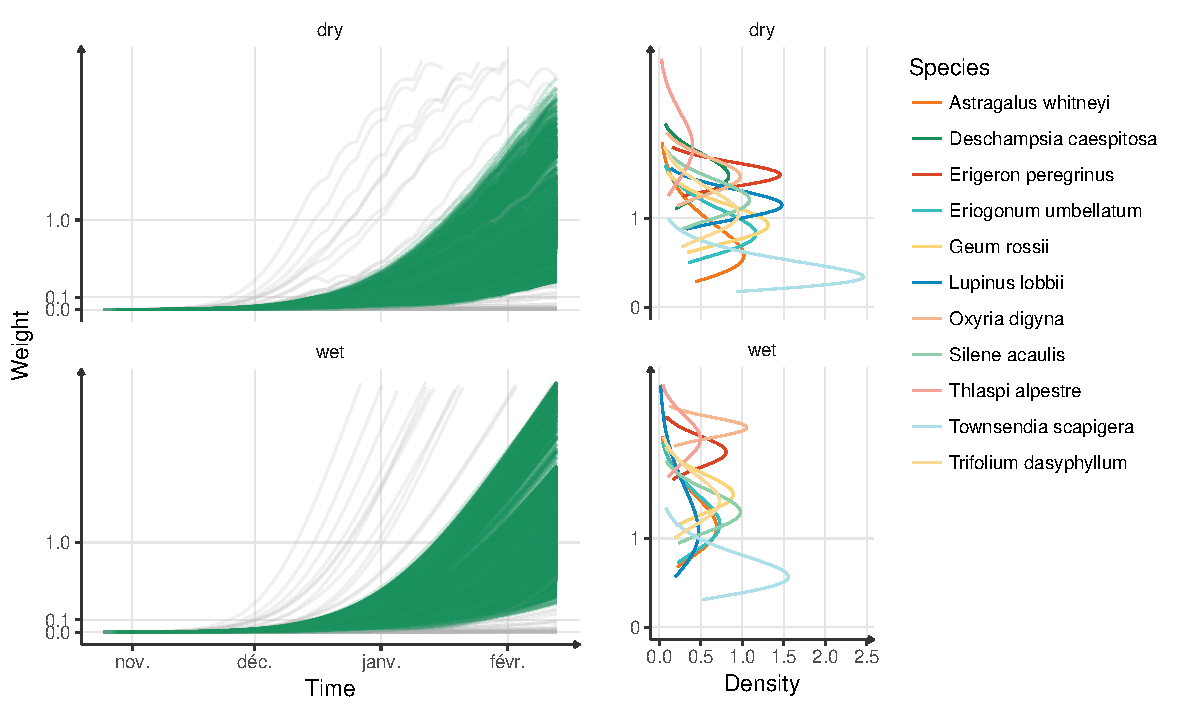
\includegraphics[width = \textwidth]{./2_PP/Figures/Calibration/weight_full_sim.pdf}
\caption{Comparison of simulated weights with distribution of weights of real alpine species for contrasting conditions.}
\end{figure*}

\paragraph{Sensitivity analysis}
Relative importance of variables in the selection process is investigated with the packages \texttt{randomForest}. A random forest analysis (depth = 5, number of trees = 300) is performed on a balance dataset composed by all selected parameter sets and a random sample of rejected sets of equal size. Importance is assessed on the results of the random forest.

\subsection{Results}

\paragraph{Selection rate}
Parameter filtering process resulted in the selection of a low number of parameter sets (below 0.2\%) for each allocation algorithms (table \ref{table:selection_rate}). This number is below the sum of accepted parameter sets per species because a parameter set can match to multiple species. Not all species contribute to the same extend to the filtering process. \textit{Astragalus whitneyi} accounts for a high percentage of accepted parameter sets, while no parameter set could match 2 species (\textit{Oxyria dignya} and \textit{Deschampsia caespitosa}). The former is characterised by wide distribution in both conditions for the two variables of interest (weight and RSR), while the latter show relatively tight distribution with little overlap between the conditions for the both variables (see figure \ref{fig:comparison_BM} for comparison between simulations and data for total weight).

% latex table generated in R 3.2.3 by xtable 1.8-2 package
% Wed Nov 15 13:39:16 2017
\begin{table2*}\label{table:selection_rate}
\caption{Acceptance rate per species for the 3 main allocation algorithms. Because some parameter sets match multiple species, the total number and rate of accepted parameter sets is lower than the sum of accepted parameter sets per species. All rates are given in \%. }
%\centering
\begin{tabular}{lrr|rr|rr}
 & & non plastic & & fixed-eq & & plastic \\
  \hline
 species & n (2M) & rate & n (2M) & rate & n (200,000) & rate \\
% species & n (995603) & rate (\%) & n (995539) & rate & n (199964) & rate \\ 
  \hline
 Silene acaulis & 227 & 0.02 & 396 & 0.04 & 55 & 0.03 \\ 
 Trifolium dasyphyllum & 271 & 0.03 &  317 & 0.03 & 45 & 0.02\\ 
 Geum rossii & 51 & 0.01 & 72 & 0.01 & 12 & 0.01\\ 
 Thlaspi alpestre & 342 & 0.03 & 360 & 0.04 & 59 & 0.03\\ 
 Deschampsia caespitosa & - & - & - & - & - & -\\ 
 Eriogonum umbellatum & 500 & 0.05 & 805 & 0.08 & 118 & 0.06\\ 
 Townsendia scapigera & 593 & 0.06 & 930 & 0.09 & 107 & 0.05\\ 
 Astragalus whitneyi & 1570 & 0.016 & 2424 & 0.24 & 318 & 0.16\\ 
 Lupinus lobbii & 678 & 0.07 &  868 & 0.09 & 123 & 0.06\\ 
 Erigeron peregrinus & 1 & <0.01 & - & - & - \\ 
 Oxyria digyna & - & - & - & - & - & - \\ 
  \hline
  Total & 4233 & 0.43 & 6172 & 0.62 & 837 & 0.42\\
  \hline
 \textbf{Accepted} & 924 & 0.\textbf{09} & 1416 & \textbf{0.14} & 200 & \textbf{0.10}\\
\end{tabular}\end{table2*}

Despite the low selection rate, a difference can be noted between the \textit{fixed-equilibrium} algorithm and the two other algorithms with a accepted rate of 0.14 \% against 0.09\% and 0.10\% (table \ref{table:selection_rate}). This difference cannot be explained by a significantly better selection rate for specific species, but rather higher rates for all species.

Most of parameter sets are not shared between the algorithms (\textit{i.e.} around respectively and third and a quarter of accepted parameter sets are shared between \textit{non plastic} allocation and \textit{fixed-equilibrium} allocation calibrations), despite that the distribution of parameter values that are not shared are very similar and do not show any clear pattern (data not shown).

Out of the 31 parameters, 6 show graphical response of selection rate (see figure \ref{fig:accept_rate}), and only  \texttt{u\_max} and \texttt{P\_max} present a possible optimum different from limit values. The relative importance of the parameters is better explored in sensitivity analysis.



%Calibration filtering results in the selection of n parameter sets over m preselected parameters sets. Accepted sets are distributed among the 11 species of the dataset like presented in the table. Species A, B and C are the most numerous.\\


%Plasticity does not change the acceptance rate in any form (only slight increased from 0.26\% to 0.38\%, up to 0.42\% for full plastic). \\


\begin{figure*}[p]\label{fig:accept_rate}
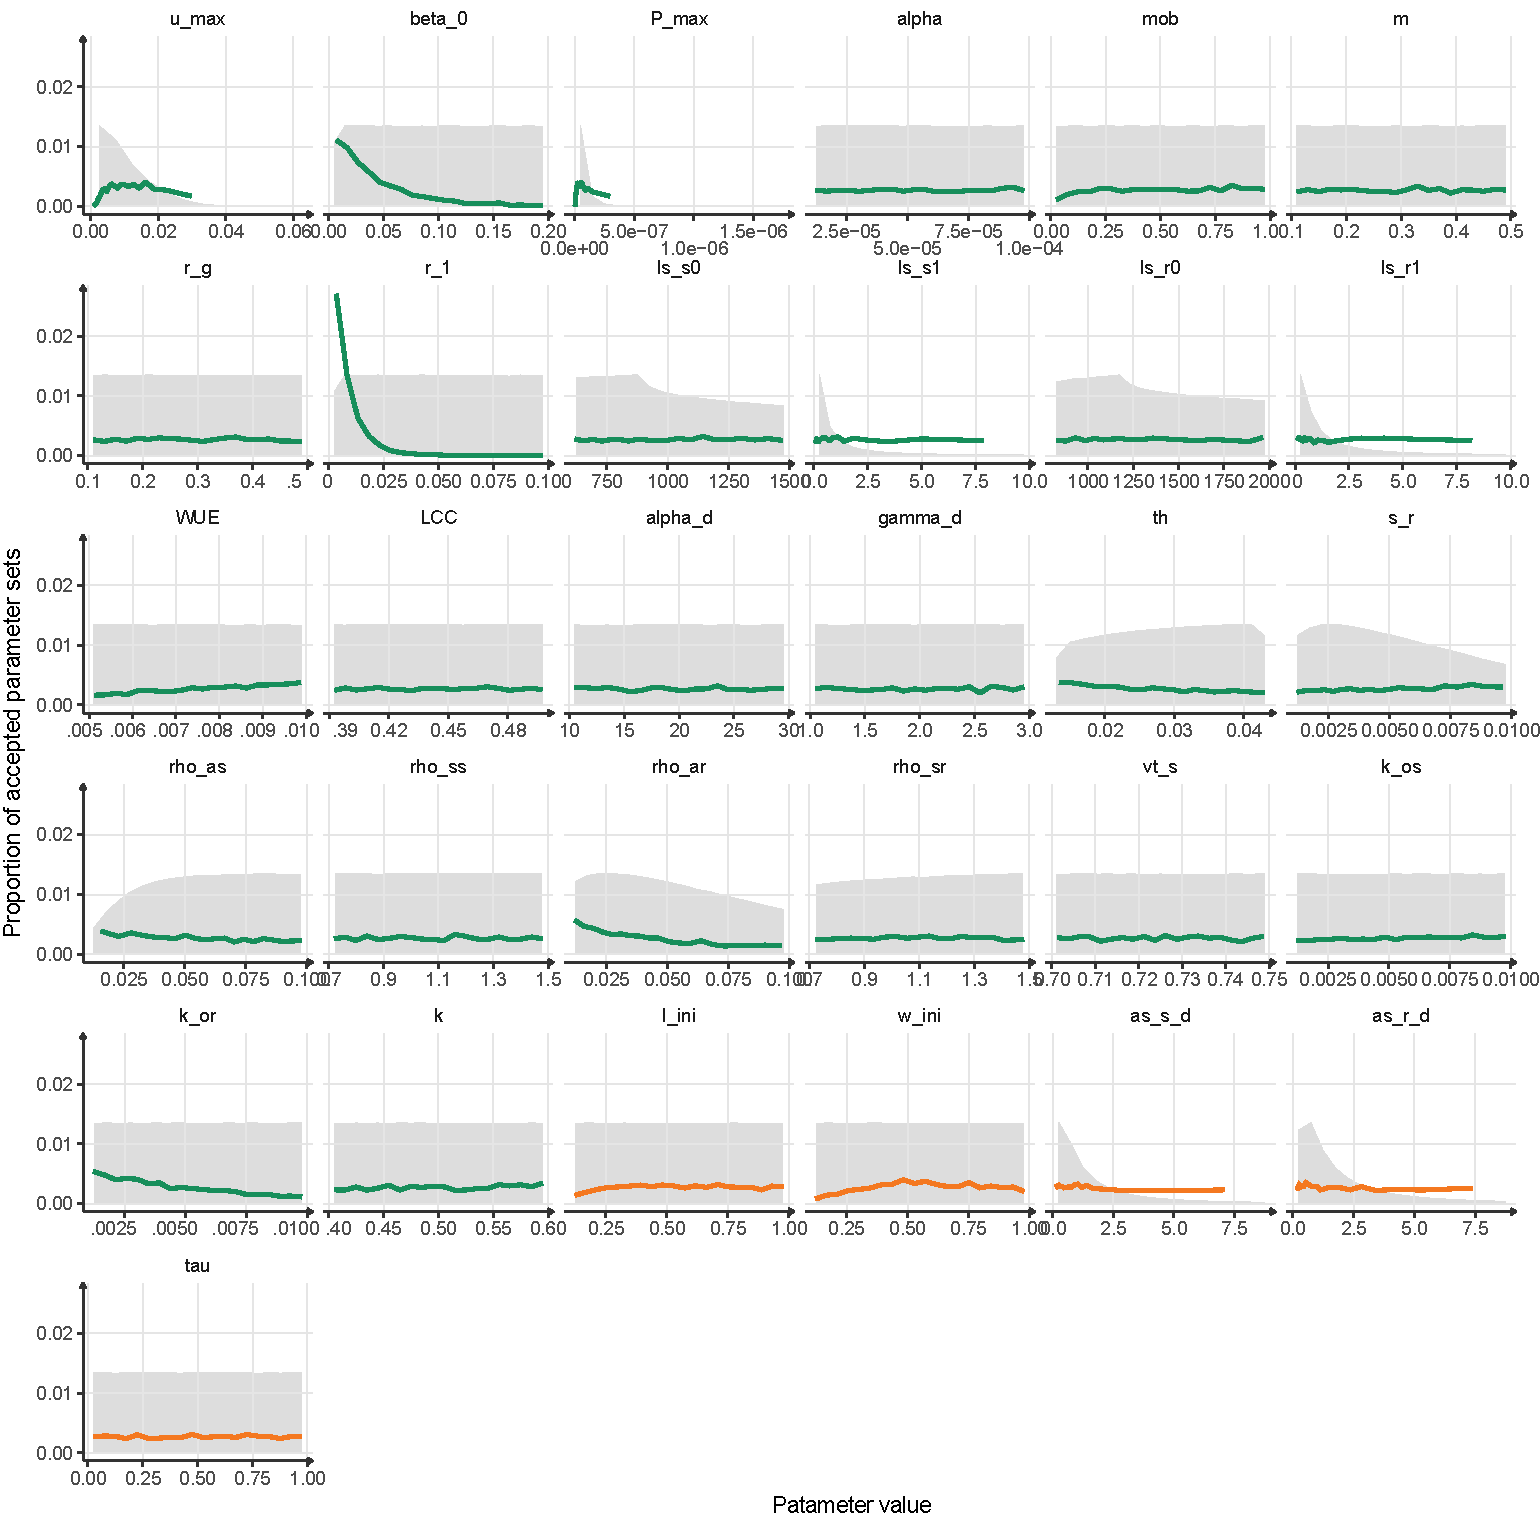
\includegraphics[width = \textwidth]{./2_PP/Figures/Calibration/acceptance_rate_RSRnWeight_per_par_none.pdf}
\caption[Selection rate of all parameters.]{Selection rate (coloured lines) per parameter  (\textcolor{myGreen}{global} and \textcolor{myOrange}{species specific}) for the individual growth. The grey area illustrates the prior distribution after the first filtering step (see method form ore details. \textit{Non plastic}.}
\end{figure*}


%\begin{figure}
%%\includegraphics[width = 10cm]{/mnt/quadri1/simulations/exploration/species_par_space2017-11-06/plots/var_imp_plot_eq_design.pdf}
%\caption{Importance of the random forest to explain filtering outcome (accepted or rejected) of a balanced sample of parameter set between all tested (all accepted parameters and an equivalent sample in rejected parameters).  Fixed-equilibrium.}
%\end{figure}

\paragraph{Sensitivity analysis}


A total of 12 parameters show a relative influence on selection rate for at least one of the algorithm. These parameters are divided between model parameters and species parameters. Species parameters show influence only for the \textit{non plastic}allocation algorithm. Model parameters express relatively similar importance for all three algorithms. The respiration rate of active tissues (\texttt{r\_1}) is the most sensitive parameters (see figures \ref{fig:accept_rate} and \ref{fig:importance}). Other sensitive parameters are related to water availability (\texttt{beta\_0}), organ exchange rates (\texttt{P\_max} and \texttt{u\_max}) and soil coverage by roots (\texttt{rho\_ ar} and \texttt{k\_or}).

\begin{marginfigure}\label{fig:importance}
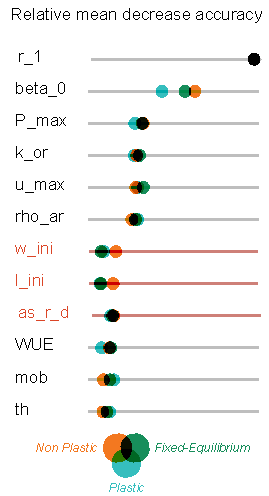
\includegraphics[width = \textwidth]{./2_PP/Figures/Calibration/importance.pdf}
\caption[Relative importance of main parameters for selection]{Relative importance of main parameters for selection under the three main allocation algorithms: (\textcolor{myOrange}{non plastic}, \textcolor{myGreen}{fixed-equilibrium} \& \textcolor{myBlue}{plastic}).}
\end{marginfigure}


%\begin{figure}[!h]
%   \begin{floatrow}
%\ffigbox{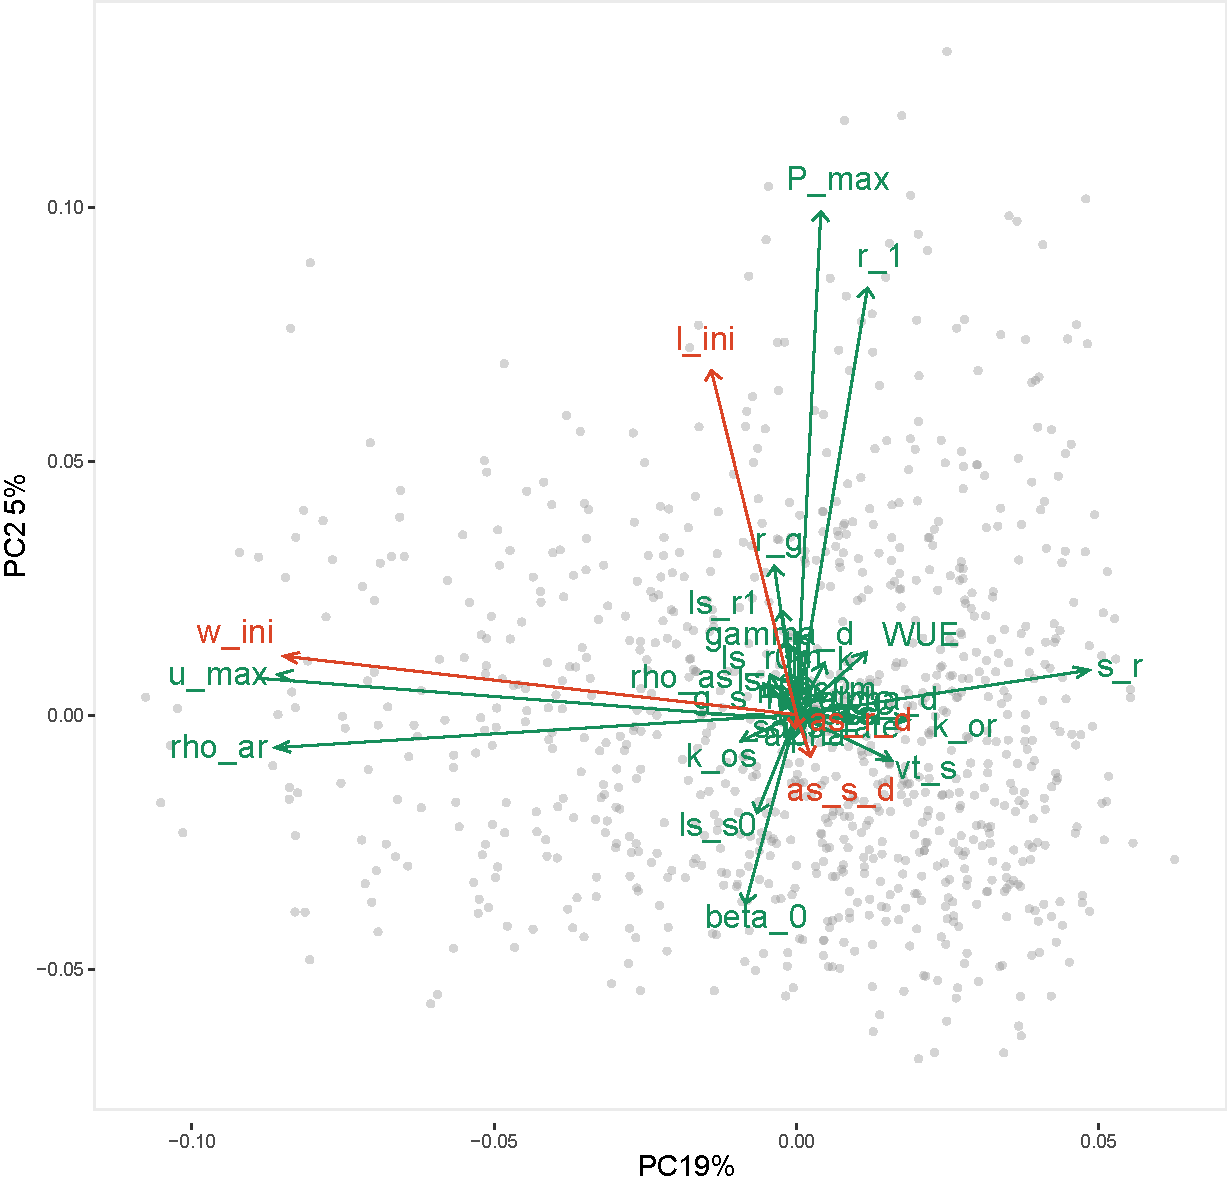
\includegraphics[width=\linewidth]{./2_PP/Figures/Calibration/PCA_none.pdf}}%
%\caption{First two axis of PCA of parameter sets selected in parameter filtering process. \textit{Non plastic}.}\label{fig:PCA_calibration}
%%       {\caption{second figure}\label{fig:example-2}}
%   \end{floatrow}
%\end{figure}
%\lipsum[3]

\begin{figure}%[tb]
    \classiccaptionstyle
\sidebysidecaption{0.60\textwidth}{0.3\textwidth}{%
    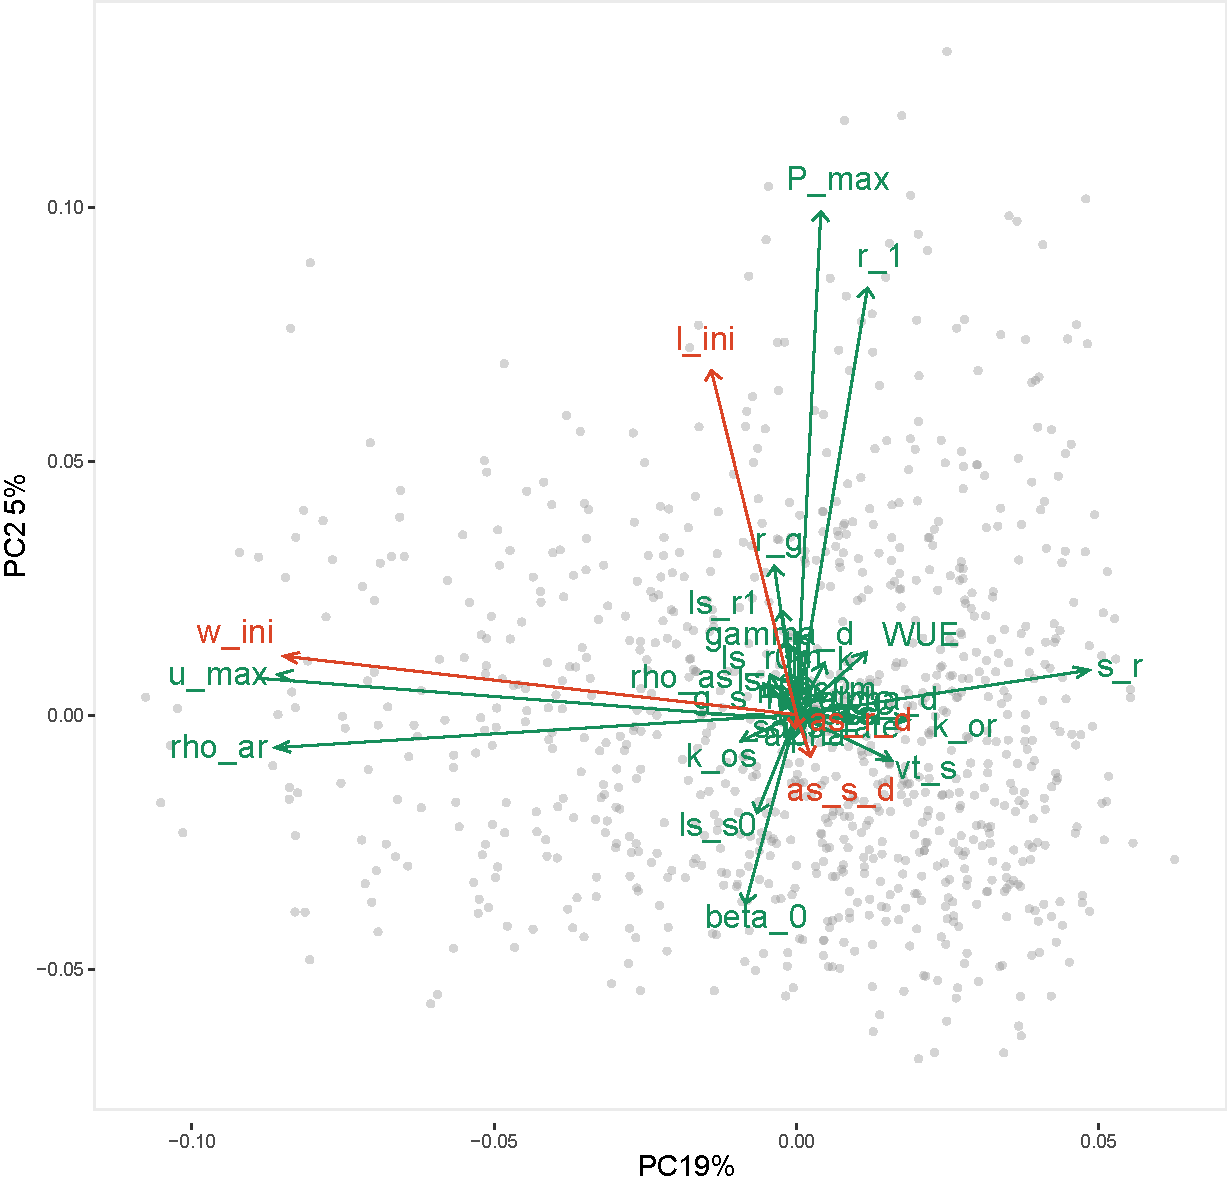
\includegraphics[width=1\linewidth]{./2_PP/Figures/Calibration/PCA_none.pdf}%
}{%
  \caption[PCA calibration]{Representation of the PCA of parameter sets selected in parameter filtering process on the first principal components. \textit{Non plastic}.}
  \label{fg:PCA_calibration}
  }
\end{figure}

The PCA performed for \textit{non plastic} algorithm only on parameter values reveals that important parameters are also the dominant variables that shapes the selected subspace. The two first axis explain only 14\% of variance. The first one is related to the root activity and efficiency (\texttt{u\_max}, \texttt{l\_ini}, \texttt{rho\_ar} and \texttt{s\_r}), the second is in line with global efficiency and resource availability.

The parameter filtering process is based on individual species, ... Species cannot be distinguished on these two main component space, neither on species specific parameters space (\texttt{l\_ini}, \texttt{w\_ini}, \texttt{w\_ini} \& \texttt{l\_ini}, \texttt{as\_s\_d}, \texttt{as\_r\_d}, \texttt{as\_r\_d} \& \texttt{as\_s\_d}) despite small variations in distribution shapes and ranges between species (data not shown).\\

\paragraph{Variable responses}
% Response of the two main vairables to main parameters.
For each algorithm the response of the two filtering variables (weight and RSR) are plotted against the most important variables in figures \ref{fig:sensitivity_BM} and \ref{fig:sensitivity_RSR}.

% Biomass
The total biomass is particularly sensitive to the tissue respiration cost (\texttt{r\_1)}, but also to the maximum exchange rate parameters. There is a notable difference in growth maxima between the two conditions in favour of the wet condition, in line with observed data. This difference is observed for the three algorithm that differ mainly by the amplitude of the biomass ranges (need data). Growth response curves are similar for all allocation algorithm. Growth is only weakly related to species specific parameters. Total biomass under \textit{Plastic-optimisation} algorithm seems to be more sensitive to variables influencing the exchange area per unit of biomass.

The species specific parameter \texttt{tau} controlling the balance between genetic and environmental control does not emerge as a influencing parameter at the global scale for any of the two flexible allocation rules.

\begin{figure}\label{fig:sensitivity_BM}
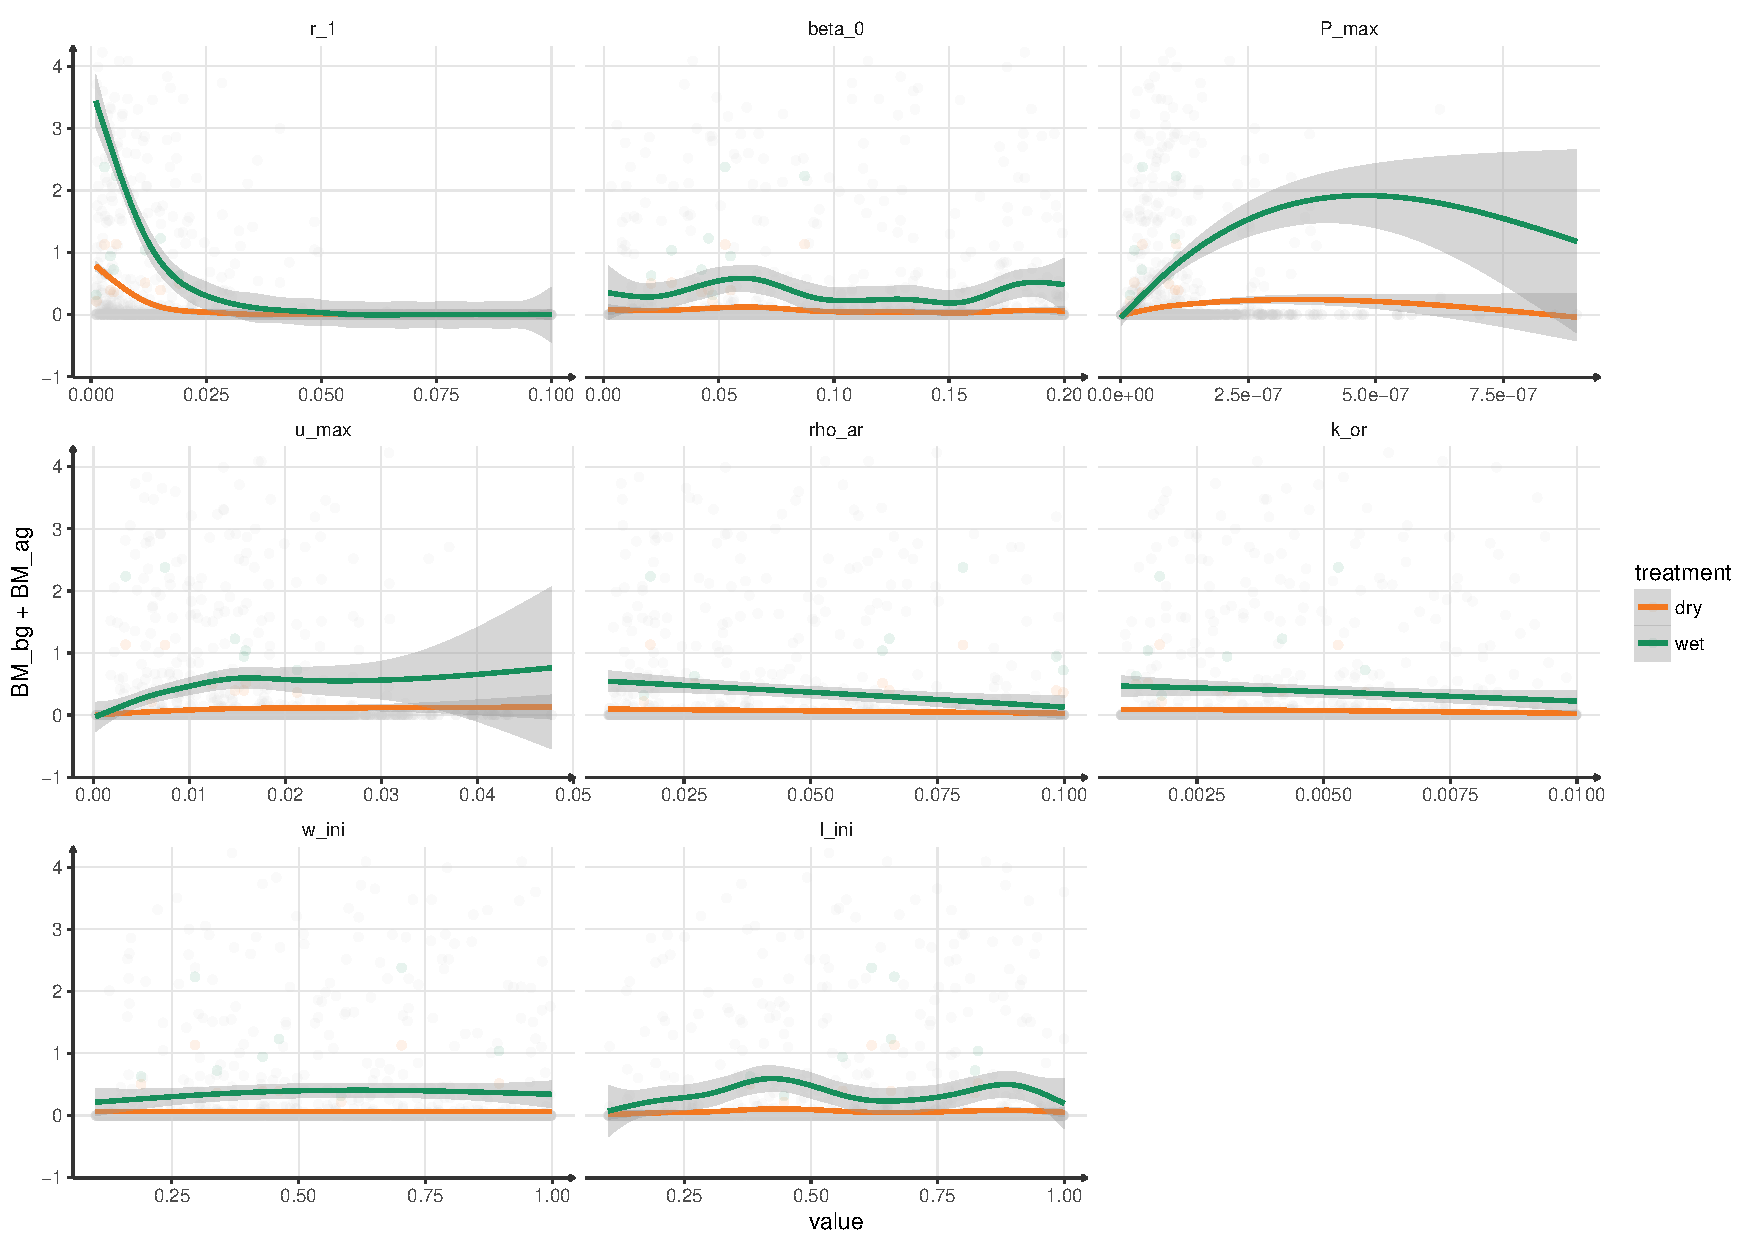
\includegraphics[width = \textwidth]{./2_PP/Figures/Calibration/par_effect_none_BM.pdf}
\caption{Main parameters effect on the total plant biomass. \textit{Non plastic}. One dot represents a parameter set. Not all parameter set are represented as the y axis is limited around the smooth function (loess). Coloured points represent selected parameter sets in the two treatments (\textcolor{myOrange}{dry} and \textcolor{myGreen}{wet}).}
\end{figure}

% RSR
Root:Shoot Ratio (or RMF in figure \ref{fig:sensitivity_RSR}) strongly responds to species specific parameters under \textit{non plastic} allocation because the memory parameters(\texttt{l\_ini} and \texttt{w\_ini}) are the means plants control their RSR. For other allocation rules, species specific parameters have little control over RSR. Surprisingly, the photosynthetic capacity has stronger influence on the ratio than the root maximum exchange rate.


\begin{figure}\label{fig:sensitivity_RSR}
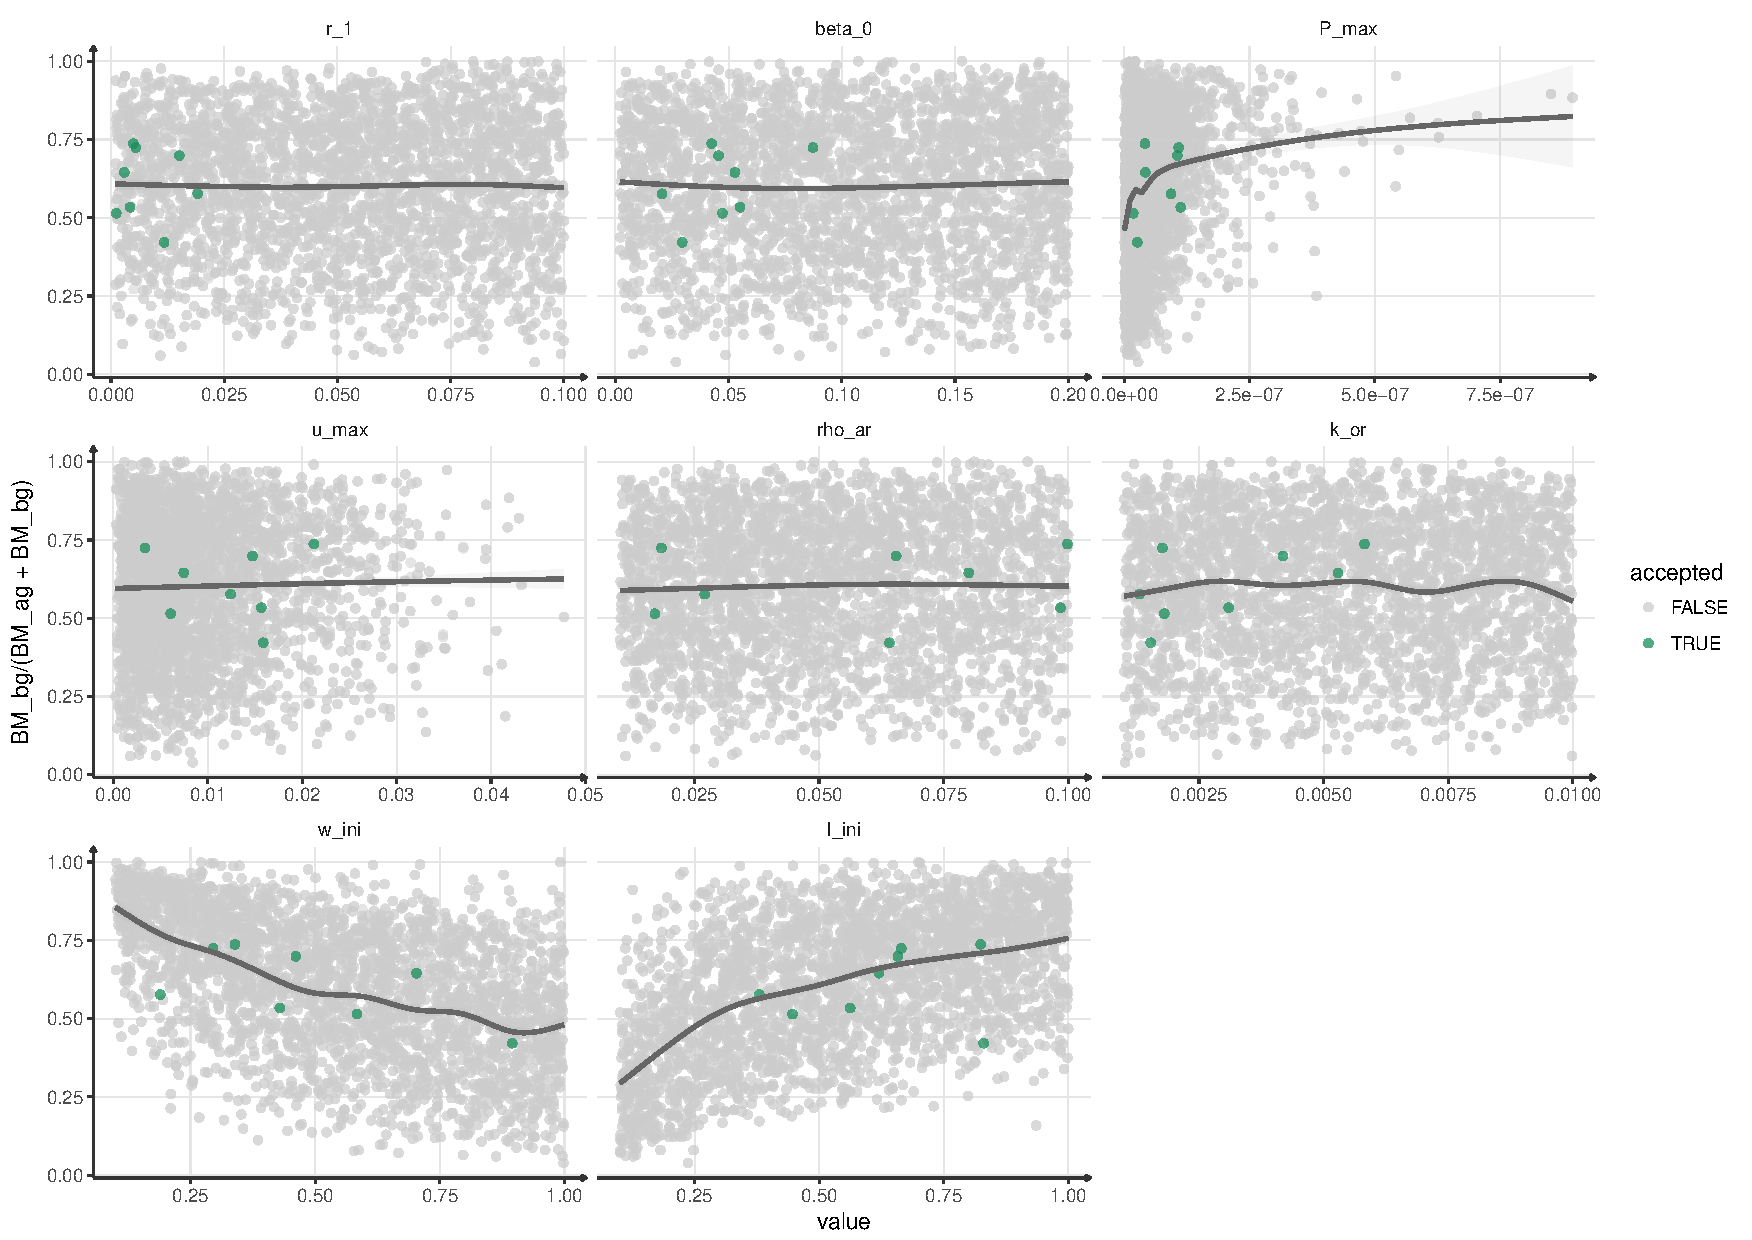
\includegraphics[width = \textwidth]{./2_PP/Figures/Calibration/par_effect_none_RSR.pdf}
\caption{Main parameters effect on the total plant Root Mass Fraction (RMF). \textit{Non plastic}}
\end{figure}

% TAU

\paragraph{Root shoot ratio and plasticity}

Little to no difference in RSR is expected for \textit{non plastic} allocation rule since allocation promoted a fixed phenotype, but both \textit{fixed-equilibrium} and \textit{plastic-optimisation} allocation rules allow for changes in RSR. Nevertheless, no stable change in RSR is observed in any of the simulations. Fluctuations are present but consist in stable oscillations between two fixed values (see figure \ref{fig:comparison_RSR}), synchronized with water variations. These rapid adaptations of the relative proportion of roots denote a high flexibility of plant phenotypes in \model.


\begin{figure*}\label{fig:comparison_RSR}
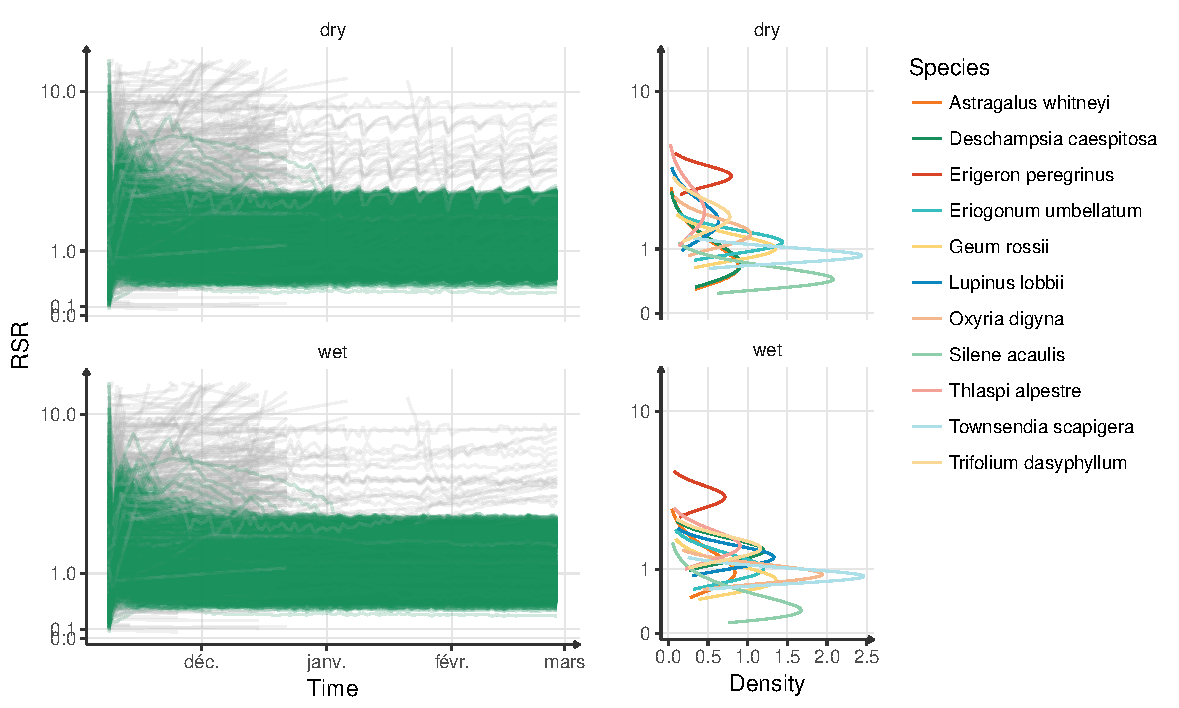
\includegraphics[width = \textwidth]{./2_PP/Figures/Calibration/RSR_full_sim_f-e.pdf}
\caption{Comparison of simulated values of RSR with real species RSR in two contrasting conditons. Because there is no plasticity or ontogeny, the simulated plant do not express any chagnes in RSR. \textit{Fixed-equilibrium}.}
\end{figure*}


\vspace{2cm}

\subsection{Discussion}

\paragraph{Growth and strategy space}

The relative low selection rates for all allocation rules highlight the complexity of fitting such complex model to empirical data, despite the relative simplicity of the data. This difficulty seems to lie in two factors: the high number of parameters and the lack of stable changes in RSR. This last point is further discussed in the following paragraphs. Nevertheless, plant growth is reproduced in two contrasting conditions for multiple species, and while plastic algorithms have a greater potential for growth (more high growth rate), this is not systematic and the absence of clear pattern for the most influencing parameters, such as maximum exchange rates and respiration rates, indicates that such high growth depends on a combination of parameter values. I believe that the shape of gain and cost functions along the functional trade-off between active and structural tissues plays a determining role in the growth. A trade-off function with a wider viable range is more likely to be selected as more strategies would grow (therefore reducing the relative sensitivity to species-specific parameters). Considering the exponential shape of the turn-over function (one of the main cost with respiration), the width and height of the trade-off (or net gain function) is probably more strongly linked to the gain functions (exchange rates) and linear cost function (respiration), explaining little effect of parameters related to lifespan (already preselected otherwise). There is a strong dependency between viable strategies (and as a consequence functional potential diversity) and the main trade-off between resource acquisition and efficiency.

Filtering the parameter sets based on all species instead of individually would have been ideal to quantify this link and better calibrate the model. However, such approach would have required many more simulations, when the parameter filtering method was chosen for its low computational cost. Moreover, considering the number of species-specific parameters, fitting the strategy subspace (at least default active tissue allocation parameters, the memory of resources and stability) of 11 species to the data in combination with more than 20 models parameters is near impossible. Ones should have had first determined the relative positions of the species within the said strategy space before any global calibration routine. Nonetheless, species-specific parameters have an influence on model main variables. Memory parameter affected the RSR in the context of \textit{non plastic} allocation rule (see figures \ref{fig:comparison_RSR} and \ref{ fig:importance}, while the default proportion of active tissues in roots was an influencing parameter in all algorithms (figure \ref{fig:importance}, \texttt{as\_r\_d}). Therefore, they should be analysed in further simulations within the same set of model parameters.

Because of the model complexity and the number of species specific parameters, in addition to long simulation time, Bayesian calibration could not be performed. In the Bayesian paradigm the information is contained in the data and revealed by the structure of the model. An alternative modelling approach is to used the parametrisation phase to accept certain parameter sets, and learn about the system through simulation experiments. The simulated data is analysed rather than empirical data. The patterns emerging from the simulation experiments inform us on the impact of the modelled mechanisms (even if they do not totally match the data). Therefore the model is still an understanding tool and can inform the effect of plasticity on ecological processes.


\textbf{The growth is reproduced in contrasted conditions, but only partially as one per parameter set is tested. The number of species and dimensions in the strategy space would not allow for a calibration of all species for one parameter set. The plastic response of the root:shoot ratio is not correctly reproduced and would require a different implementation (stress based). However the plasticity as implemented improved the acceptance rate because of a better growth. Therefore the effects of plasticity can still be investigated with simulation experiments.}

\paragraph{The role of water}

If the parameter filtering step does not result in the selection of optimum values for all parameters, it provides information on the main mechanisms influence plant growth. Indeed, the relatively high importance of parameters related to water shows the importance of the resource on the model behaviour. Both water availability (water absorption limitation, exchange rate) and root mass and construction parameters are important to match the empirical data. Considering that the calibration relies on experiment data of drought events, it is no surprise that parameters related to water economy show strong influence on the selection rate and model behaviour. In the context where the model has been developed, water shortage is expected to be an important factor for the community dynamics. In this perspective, the ability of \model to reproduce the differences in productivity between both conditions, and the relative sensitivity to water related parameters is an advantage. The link between water resource, species strategy, plant performance and phenotypic plasticity is explored more in details in the following section.


%Differences between algorithms that make sense: more biomass, sensitive parameters are related to how plasticity work...

\textbf{The sensitivity of the different variables to the parameters align with the two criterion of selection (that work with the independence of trade-off). In contrast with forest, the light is not the most important factor and water plays a more limiting role. A particular focus on below-ground resources should drive the simulation experiments with this model.}

%\paragraph{More complex plasticity?}

\paragraph{Phenotype flexibility}

As mentioned earlier in this discussion, the model is not able to produce any shift in RSR in different water treatment. It is not a surprise for \textit{non plastic} algorithm, but the filter was still applied on this criterion to allow the comparison with plastic algorithm and to be able to measure the improvement in selection rate. However, even plastic algorithms do not show strong enough response to water treatment in term of RSR. A strong and good (in the sense it would have matched the data) is larger in amplitude and more stable in time. Such processes generally amplify with time, \textit{i.e.} when the number of drought event increases, the response (allocation to roots) increases (relative to default phenotype). Unlike natural systems, plants in \model fluctuates between two "states", or phenotypes associated to the dry and the wet conditions. The value of the RSR followng a drought event is reached after the first week without water. This can be explained by two main mechanisms that are related but have contrasting implications. The quickness in response to the changing conditions is allowed by relatively high assimilation rates. While the net growth rate is limited by the comparison during the filtering process of the total weight of plants with the empirical data, the assimilation rate is not and can be compensated with relatively high turn-over rate. Net growth rate being equal, species with higher assimilation rate will have higher \textemph{phenotypic flexibility} (higher fraction of biomass to invest in carbon pool of choice) than species with lower assimilation rate (but lower turn-over. This flexibility, similar to reallocation, allows changes in RSR, but not the accumulation of biomass in roots. Unfortunately, both the constant turn-over rate implemented in the model, and the selection toward "wide and high" gain functions limit control on this aspect.

This generalised high phenotpic flexibility allowed by high assimilation rates to compensate high turn-over rate highlight a problem within the calibration. The reproduction of growth patterns gives us confidence in the good functioning parameter filtering process, so wrong priors are certainly the cause of this behaviour. The uncertainty around the exchange rates for shoot and roots lead to the definition of relatively wide priors informed by parametrised models \parencite{kleidon_global_2000, reineking_environmental_2006, taubert_modelling_2014}. In the other hand, the turn-over parameters are relatively well informed by modelling appraoches but also empirical studies \parencite{ ryser_ecological_2000, wright_worldwide_2004, tjoelker_linking_2005,  luke_mccormack_predicting_2012}, leading to more constrained priors. The value of these priors is not discussed, it is rather how they are translated within the context of the model leading to an over-estimation of the cost of leaf senescence. Because the lifespan is integrated at the daily time-step as a constant turn-over rate, instead of a late decrease in biomass as in natural systems, the biomass is reduced early in the growth (from day 0). This can be a problem when the growth is non linear, especially when growth is higher early in the growth period. In this context, fairly narrow priors can lead to an over-estimation of the turn-over cost as the non linear growth is not properly integrated by the integration of the tissue senescence. This over-estimation is then compensated, during the parameter filtering process by a higher assimilation rate and a higher tissue flexibility.

The particular design of the experiment from \cite{peterson_growth_1982} with cycling wet and drought periods can also explain this effect. Other experiment designs with shifts in the mean influx of water would limit the role of the phenotypic flexibility and show more consistent differences in RSR between wet and dry conditions.
% is not the priors value that is discussed, but how it is translated in the model, and how in combination with relatively narrow priors, limit the emergence of stable RSR differnces due to inertial.


Moreover, the fact that plants are more productive during periods where they may not want to invest in roots reduces the possibility for a strong duragble shift of RSR. Indeed, a plant would drift to higher RSR if it was more productive when pursuing the high RSR phenotype than when pursuing the low RSR phenotype. This last point mentions the "will" of the plant, in the context of \model this target-phenotype is encoded in the projection of external conditions. Because this projection is daily based by design, the accumulation of drought stress is not translated in the internal projection variables of the plant (like it can be with the accumulation of phyto-hormones.). This limitation highlights a big difference between simulated plants in \model and natural plants. While solutions to overcome this problem can easily be imagined(see equation \ref{eq:projection_alt} in \ref{subsection:submodels}), they would require more parameters and introduce more complexity to the analysis. This model provides a first approach to phenotypic plasticity in grassland models and the formulation of the projection, key element of the phenotypic plasticity, is certainly a starting point for further development. Nevertheless, the differences in response to the parameters between the three allocation rules, despite shared plant functioning, demonstrate the importance of plasticity itself. And simplification of the processes should not be a reason to not explore its effects. The fact that the parameter \texttt{tau} has a relatively small impact on selection rates alos support the need to better understand all strategic axis before focusing on the effect of projection. While there are many ways of simulating the phenotypic plasticity, the parsimony is privileged. This simple representation is enough to understand the effects of active plastic allocation in association with the other strategic differences between species.

\textbf{The high flexibility of the plant phenotype given by the high assimilation and turn-over rates reduces the inertia of the model and its capacity of modelling lasting changes in RSR. The modelling of the plastic response also reduces the capacity of the model to well capture changes in RSR. }\\

\textbf{The parameter filtering process successfully capture the growth pattern, showing convincing patterns of parameter sensitivity and variable response. However, limitations in the plastic response modelling, coupled with high phenotypic flexibility and a particular experiment-design do not allow a solid representation of the RSR differences between the conditions. Nevertheless, the \model still offers a way to interrogate the effect of plasticity on growth patterns, optimum strategies and potential diversity.}
%Exchange area per biomass and sensitivity to exchange rates : trade-off are important and structuring.

%filtering on RSR to test if plasticity improved selection of parameters, = is an essential part of platn functioning.\\
%\paragraph{Modelling paradigm}
%Bayesian paradigm where the information is contained in data and revealed by the structure of the model. Go for simulation experiment approaches where the model is used as a simulation tool and results as new data. The emerging patterns inform us on the impact of the modelled mechanisms (even if they do not totally match the data). Model as an understanding tool.\\
%While many ways of simulating the phenotypic plasticity can be proposed, the parsimony is privileged and this representation is enough to understand the impact of related processes shared by any representation of phenotypic plasticity is the developed framework.

%\textbf{Root shoot ratio changes were not captured by the model. The structure of the plasticity mechanisms does not work with the given watering cycle. Needs to add one parameter for reactivity.}



% ##################################################################################
\section{Individual level behaviour and properties of plastic allocation algorithm driven by the plant memory}


Calibration and sensitivity analysis give information on the main processes of plant growth, but the general effects of the allocation rules on plant growth are not fully identified. Moreover, because the parameter filtering processes was limited to individual plants and the effects of the species specific parameters are depending on the other parameters of the model, the effects of these species specific parameters should further be investigated. The objective of this part is to set better understanding on the role of the \textemph{allocation rules} and species \textemph{memory} on plant development as basis for interpretation of plasticity effects in following chapters.

The challenge of the framework presented in the paragraph \ref{subsection:memory} under \textit{plastic-optimisation} is to control the phenotype with the values of the memory. The risk of this approach is to have too tight estimation function of the fitness (or driving function) and to see the convergence of all species (with different memory values) toward the same phenotype (same allocation of active and structural tissues in roots and shoot). The extend to which different species memory lead to different phenotypes under full genetic control (not influenced by the external conditions) is explored through simulation experiment under \textit{plastic optimisation} allocation algorithm with no effect of conditions on traits ($\tau = 1$), only on growth.

%Proof of concept
\subsection{Method}


%\paragraph{Strategy diversity filtering}
%To further reduce the number of parameter sets considered, we proceeded in an additional filtering step. Because the first filtering was conduced for only one strategy over the whole 4D strategy space (l\_ini,  w\_ini, as\_s\_d, as\_r\_d) it is necessary to verify that other strategies do not lead to potential Darwinian demon. This should be limited by the choice of priors, while at the same time promoted by the selection of parameters increasing growth to counter balance potential unfitted strategies\footnote{Better do that beforehand than after... But I guess it's too late now.}.

\paragraph{Allocation algorithms}
The effect of allocation rule on phenotypic development is investigated thanks to pot simulations (see Methods in \ref{section:calibration}) of 100 days in 3 watering treatment: 2mm, 8m and 16mm per day. To avoid drift in the phenotype due to allocation algorithm (see paragraph \ref{subsection:memory} on phenotypic determination), simulations where run a first time, then rerun with default specific traits matching traits at the end of the first simulation set. All four algorithms are simulated. To reduce the number of simulations 100 parameter sets are selected randomly within the accepted parameter sets for the \textit{non plastic algorithm}.

\paragraph{Memory \& phenotype}
Memory of external conditions plays a determining role in phenotypic development under \textit{plastic-optimisation} allocation rules. The effect of the memory alone (environmental cues ignored by setting \texttt{tau} to 1) on the default emerging phenotype is explored for diverse memories (9 values on the two axis from 0.1 to 1 later scaled to the maximum area exchange rates for model parameter set considered, or 81 values) for each accepted parameter set. The effect of the memory values on the final position of plants in the phenotypic space are visualised by fitting loess curves between memory values and individual trait values.

\subsection{Results}

\paragraph{Allocation algorithms}

\begin{figure}\label{fig:allocation}
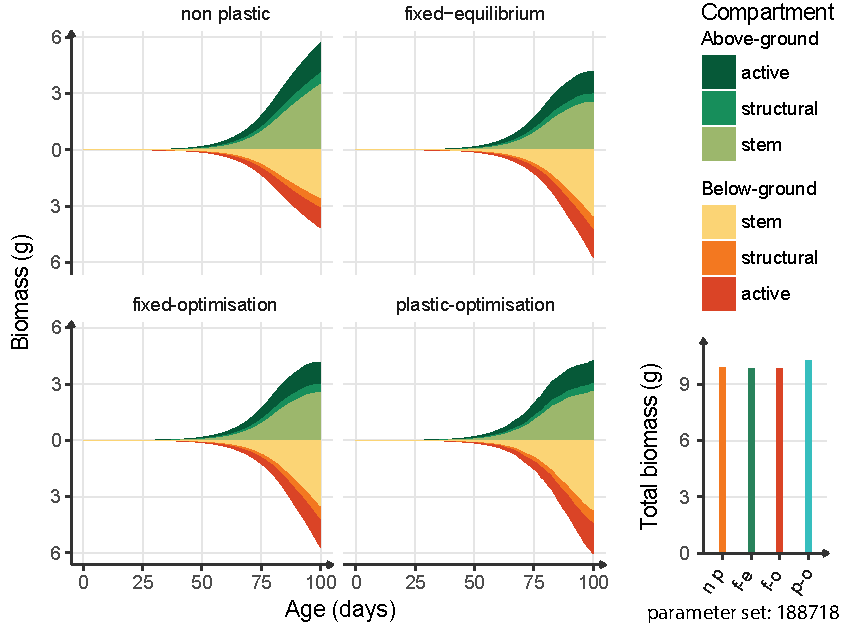
\includegraphics[width = \textwidth]{./2_PP/Figures/Individual/allocation_rules.pdf}
\caption[Effect of the different allocation algorithms on the different biomass compartments]{Effect of the different allocation algorithms on the different biomass compartments of the plant. The fraction of organic matter allocated to the stem (ensemble of supporting tissues for shoot and roots) are increasing over time for all algorithms. The \textit{non plastic} algorithm show constant allocation coefficients between above-ground and below-ground compartments and between active and structural tissues. All others show different coefficients for the above-ground - below-ground partitioning, and the \textit{plastic-optimisation} algorithm have changing proportion of active and structural tissues. The bottom-right panel show the total biomass for the four allocation algorithms after 100 days. }
\end{figure}


%think of a "showtime" visualisation that shows how growth and traits are impacted by allocation rules and \texttt{tau}.\\

The allocation algorithm affect the way the organic matter in distributed between the different tissues of the plant. With partitioning coefficient pre-established for the given conditions, the algorithm show very similar performances (see figure \ref{fig:allocation}). The difference in allocation algorithm is mostly noticeable in figure \ref{fig:allocation} mostly on the shift toward root allocation at the end of the simulation when the water becomes to be limiting. The plant under \textit{plastic-optimisation} allocation benefit from a light improvement in performance (mean: +10\%, median: +3.4\% relative to \textit{non plastic}).

The \textit{plastic-optimisation} algorithm allows changes in the proportion of active tissues in organs. This may have repercussions on the allocation between shoot and root, but also can lead to non specific variability within plants with no perception of resource fluctuations ($tau = 1$). The median variability of the RMF (root mass fraction) along the 100 simulated days is 0.015, that is five times higher than the variability of the other plastic algorithms (\textit{fixed-optimisation} and \textit{fixed-equilibrium})(see table \ref{table:variability-rmf}). This variability is much higher (around 0.028) for the plastic plants in all three plastic algorithm, while it is null for the \textit{non plastic} allocation rule. The range of the RMF follows similar trend, with higher value for the \textit{plasti-optimisation} than the other algorithms when plant do not perceive the resource fluctuations, and wide range for all plastic allocation algorithms when plants take into account the changes in light and water resources.

\begin{table}[h]
\centering
\caption{Median of variability and range of the RMF for simulations of 100 days, for 100 different parameter sets and three different water treatments (2, 4 and 8 mm per day), in the four different allocation algorithms. sd: standard deviation.}
\label{table:variability-rmf}
\begin{tabular}{l|ll|ll}
            & \multicolumn{2}{c}{\textbf{sd}}              & \multicolumn{2}{c}{\textbf{range}}           \\
\hline
\textbf{algorithm}                     & tau = 0          & tau = 1          & tau = 0          & tau = 1          \\
\hline
none                 & $<10^{-12}$ & $<10^{-12}$ & $<10^{-12}$ & $<10^{-12}$ \\
fixed-equilibrium    & 0.0278           & 0.00212          & 0.173            & 0.0155           \\
fixed-optimisation   & 0.0279           & 0.00221          & 0.173            & 0.0161           \\
plastic-optimisation & 0.0283           & 0.0150           & 0.174            & 0.0839          
\end{tabular}
\end{table}

The plastic algorithms show similar levels of variation and range, while the \textit{non plastic} one is stable as expected. The \textit{plastic-optimisation} allocation show more instability for non plastic plants ($tau = 1$) but that is lower than the variability observed in plastic plants ($tau = 0$). The allocation (and therefore phenotype) is controlled by the allocation rules (plastic dimensions and objective functions) and the estimation of conditions. Before investigating the effects of varying conditions, it is important to understand the effect of memory on plant strategy and phenotype.

%Have the proportion of tissues changing over time\\

%Show the respiration, assimilation and turn-over rates.\\ 

%Isn't it possible to show these along memory or active/str ratio axis ?


\begin{figure}\label{fig:plastic_allocation_trajectory}
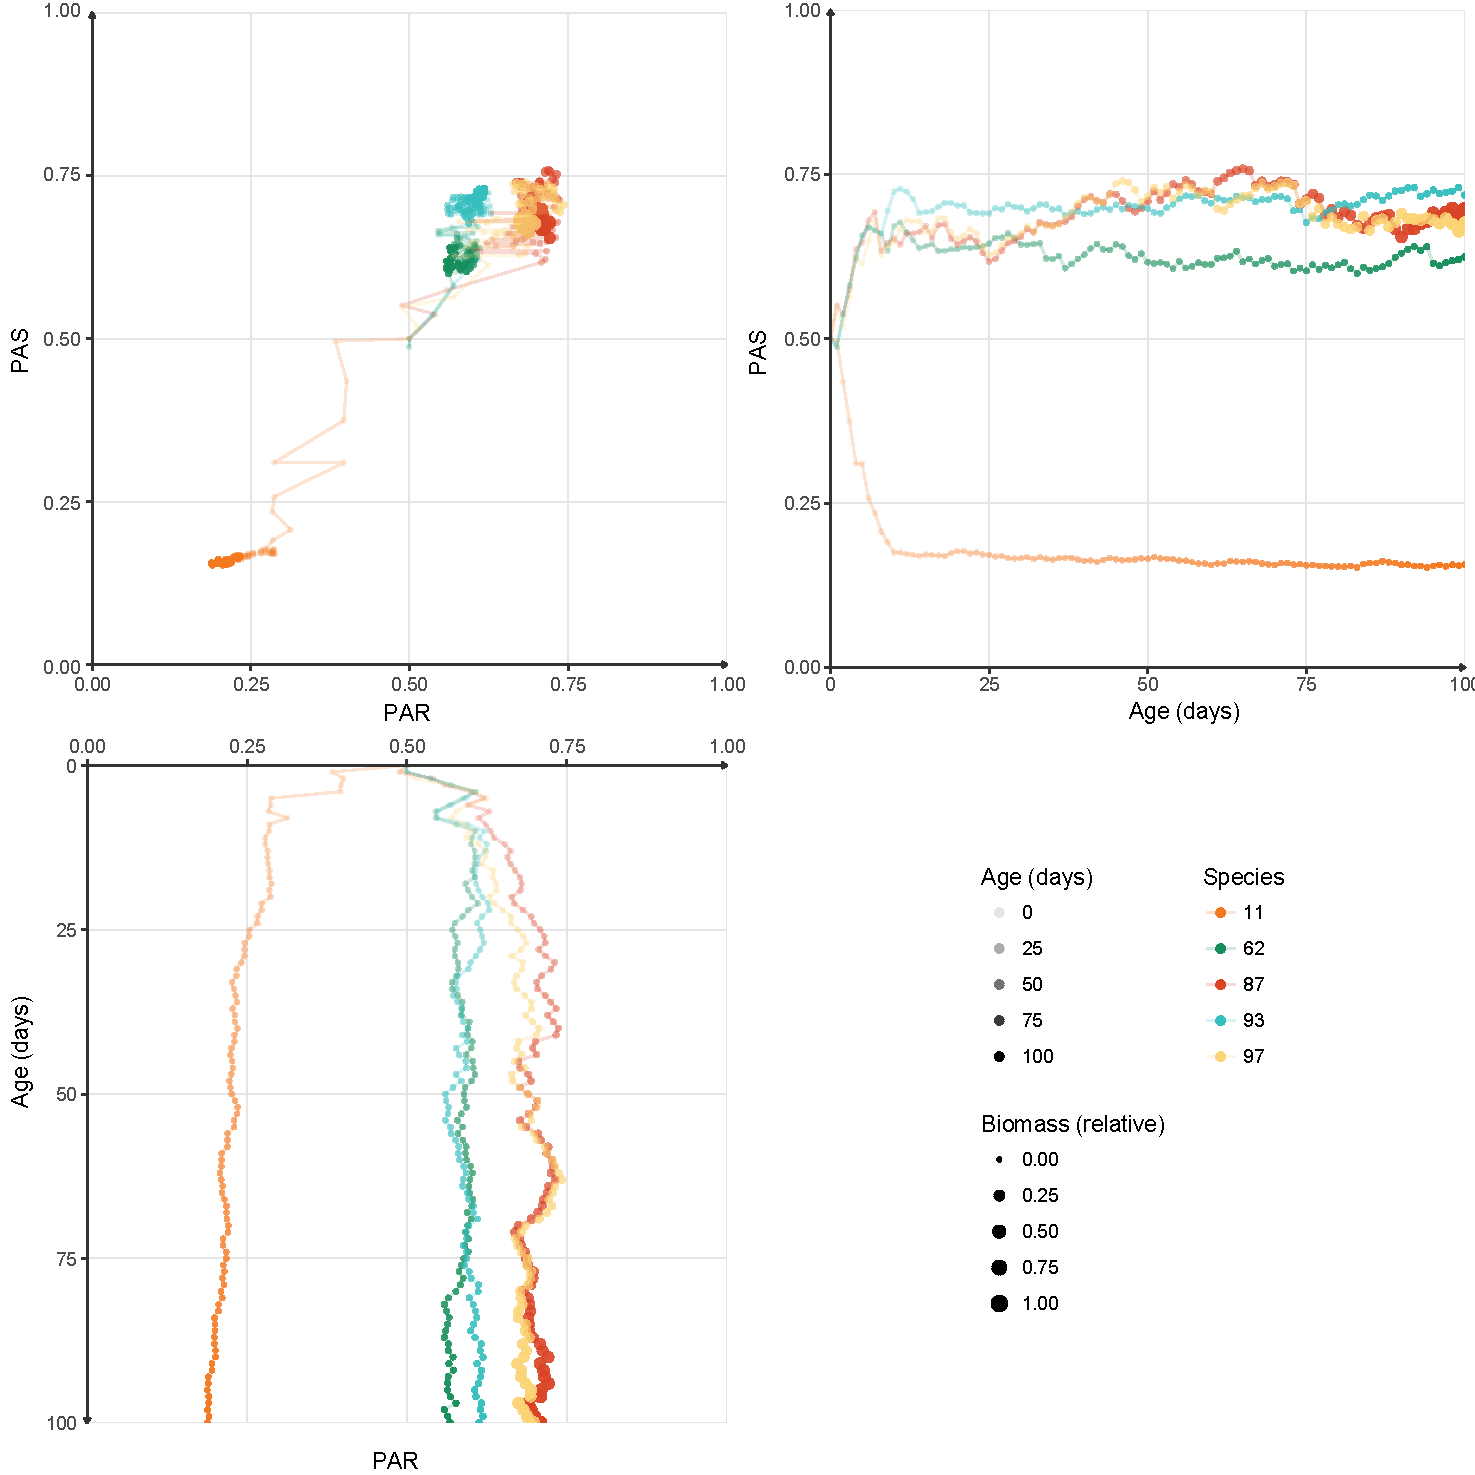
\includegraphics[width = \textwidth]{./2_PP/Figures/Individual/memory_effect.pdf}
\caption{Trajectories along time in the strategy space of 5 plants with different memories. After 10 days, all plants have converged toward the estimated optimum.}
\end{figure}

\paragraph{Memory and phenotype}

The kinetic of the phenotypic shift is first visualised for one parameter set on the two main phenotypic axis (proportion of active tissues in roots: PAR and proportion of active tissues in shoot: PAS). From the same starting point the five species show distinct rapid shift toward segregated subspace of the 2D strategy space. The equilibrium point is reached in approximately 10 days for all 5 species. Despite constant memory, variations are visible on both tissue allocation traits of roots and shoot. These variations lead to partial overlap but the five species are distinct on the 2D space.

The memory of resource availability is a strong enough driver to alter the default phenotype of a species. The effect of the two components of the memory (memory of water availability and memory of light availability) on the three main traits is explored through local regressions. The proportion of active tissues in roots increases to a plateau with increase in water availability memory (figure \ref{fig:w_ini_p_as_r}). This response pattern is consistent between all parameter sets, but the starting points and slopes may differ. The same pattern is observed between light availability memory and proportion of active tissues in roots (data not shown). The allocation convergence in the root is also influenced by the increase in light availability memory. An increase in the latter leads to a smooth increase in the former (see figure \ref{fig:l_ini_p_as_r}) with less drastic response than the water. This response is mirrored in shoot allocation response to increase in water availability memory (data not shown). Both organs react in symmetric ways to increases in resource availability. The RSR has a negative log response to water availability memory (positive in the case of light availability memory).

\begin{figure}\label{fig:w_ini_p_as_r}
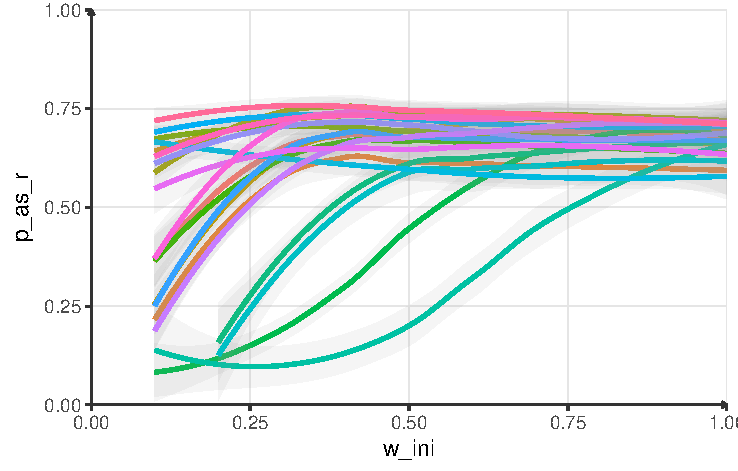
\includegraphics[width = \textwidth]{./2_PP/Figures/Individual/w_ini_p_as_r.pdf}
\caption{Effect of memory of water availability on proportion of active tissues in roots. \textit{Plastic-optimisation}. Each line correspond to a local regression fitted for all memory combinations for a given parameter set. Water availability memory is given in percentage of maximum exchange rate, absolute values may change between parameter sets.}
\end{figure}


\begin{figure}\label{fig:l_ini_p_as_r}
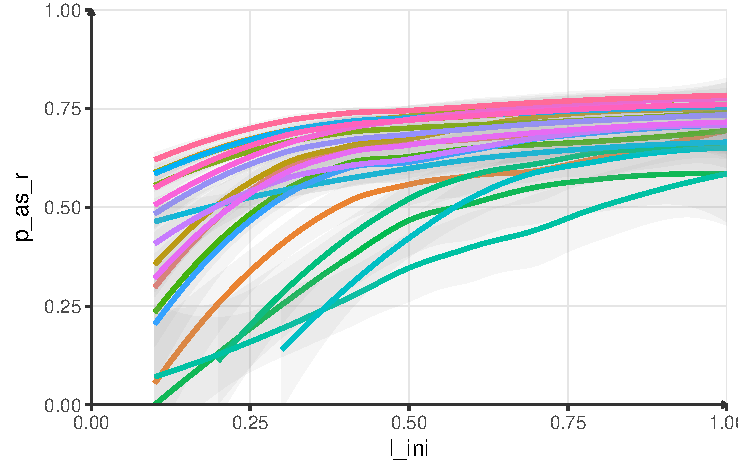
\includegraphics[width = \textwidth]{./2_PP/Figures/Individual/l_ini_p_as_r.pdf}
\caption{Effect of memory of water availability on proportion of active tissues in shoot. \textit{Plastic-optimisation}. Each line correspond to a local regression fitted for all memory combinations for a given parameter set. Light availability memory is given in percentage of maximum exchange rate, absolute values may change between parameter sets.}
\end{figure}

The combine effect of the two axis of plant resource availability memory is observed by plotting the phenotypes (on the 2D space of active tissue allocation) of four contrasting memories for all parameter sets (figure \ref{fig:memory_n_phenotype}). There is clear clustering of the four memory profiles, with some overlaps due to the fact that multiple parameter sets are plotted at the same time. The memory of low availability (\textcolor{myRed}{$\bullet$}) has a much larger distribution area than others, suggesting the relative instability of this profile within the "estimated net gain landscape". Memory of low availability for both resource drives plant toward very conservative strategies (need some values here) than other strategy. High expected availability of at least one resource increases allocation to active tissues to both organs. This confirms the positive effect of complementary resource (light for roots and water for shoot) of active tissue allocation in organs (see figure \ref{fig:l_ini_p_as_r}). Because of this, there is no highly unbalance phenotypes with high contrast between organ specific allocation emerging from the \textit{plastic-optimisation} allocation in \model. There is general coordination, but the balance between resource availability memories still impacts the position on the 2D, illustrated by the absence of overlap between low light - high water  (\textcolor{myBlue}{$\bullet$}) and high light - low water (\textcolor{myYellow}{$\bullet$}) phenotypes. In case of high resource availability and coordination, high investment in active tissues for both organ is achieved(\textcolor{myGreen}{$\bullet$}) and high light - high water), but the range of values is similar than for unbalanced memories(\textcolor{myBlue}{$\bullet$}) and high light - low water (\textcolor{myYellow}{$\bullet$}).

\begin{figure*}\label{fig:memory_n_phenotype}
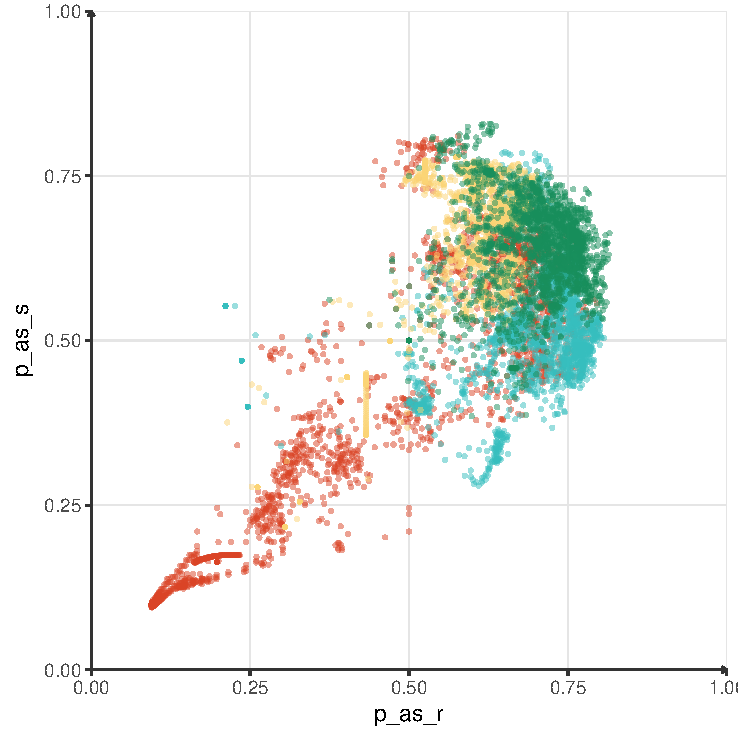
\includegraphics[width = \textwidth]{./2_PP/Figures/Individual/par_v_2D_points.pdf}
\caption{Impact of species memory on final phenotype in case of fully plastic allocation. \textit{Plastic-optimisation}. Each point corresponds to a plant phenotype for a memory syndrome for a given parameter set. Colours denote the memory syndromes.

\textcolor{myRed}{$\bullet$ low light - low water}, 

\textcolor{myYellow}{$\bullet$ HIGH light - low water},

\textcolor{myBlue}{$\bullet$ low light - HIGH water},

\textcolor{myGreen}{$\bullet$ HIGH light - HIGH water}.}
\end{figure*}



\subsection{Discussion}

\paragraph{Allocation algorithms}

The pre-calculation of phenotypes, avoiding any phenotypic drift, allows for all allocation rules to grow plants with close performances. Nevertheless, the plastic algorithms show changes in RMF at the end of the simulation when the light:water balance starts to shift. This consistent shift in RMF for all three plastic allocation rules (with low variation of the other plastic dimensions) suggests the sensitivity and importance of this phenotypic axis. On the other hand, the other plastic dimensions benefit the plant growth suggesting that they also play a role in the tissue efficiency. While both the RMF and the proportion of active tissues can change the exchange area, only the proportion of active tissues can change the tissue efficiencies. Because the RMF shows similar levels of variation and range in both \textit{fixed} algorithms (RMF is the only plastic dimension) and \textit{plastic-optimisation} algorithm (see table \ref{table:variability-rmf}) the allocation of active tissue in the latter algorithm does not compensate for change in root:shoot allocation and is not used to increase the area of the limiting organ. This is confirmed by the fact that memory of low-light conditions (\textcolor{myBlue}{$\bullet$} in figure \ref{fig:memory_n_phenotype}) lead to lower allocation to active tissues than high light conditions (\textcolor{myYellow}{$\bullet$}). In the case of fully plastic plant trying to optimise their growth, the vegetative phenotypic dimensions do not fulfil the same functions: the RMF is used to adjust the balance between the resource exchanges while the change in active tissue proportions are related to the tissue and whole plant efficiency. This contrast in functions looks opposed to what is often observed in empirical studies wher eshoot:root ratio and SLA (here controled by the porportion of active tissues) respond in the same direction to increase the leaf area and compensate low indident light \parencite{ryser_consequences_2000, poorter_causes_2009, poorter_biomass_2012}. This discrepency reveals a limitation within the plastic-allocation algorithm: the balance function is mostly supported by changes in root:shott ratio while the proportion of active tissues (controlling SLA and SRL) controls the tissues efficiency. The low proportion of active tissues in low resource (\textcolor{myRed}{$\bullet$} in figure \ref{fig:memory_n_phenotype}) indicates a selection of more conservative phenotypes when the resource is scarcer. This is in agreement with the Grime's triangle \parencite{grime_evidence_1977} and large scale empirical studies \parencite{wright_worldwide_2004}. In contrast with the conclusions of \cite{ryser_consequences_2000}, here the full phenotypic plasticity of the \textit{plastic-optimisation} algorithm is driven by similar constraints than the long term selection processes. This can be explained by the design of the trade-ofs that drive the gain function (see chapter \ref{part:model}). Therefore there are strong constraints on the tissue allocation, but low constrains on the root-shoot allocation. Additional constraint of this dimension can be added by considering other functions of each organs (such as nitrogen absorption by roots), or more artificially by increasing the cost of the displacement along the RMF axis. The fact that traits and allocation may be constrained in different way has been observed by \cite{freschet_integrated_2015}, highlighting contrasted types of response between shoot and roots \parencite{poorter_limits_2015}. Also, it appears here that studying the long term effect of a fixed estimation of conditions is probably not the best way to understand how the plastic responses of plants to an abrupt change in conditions. However, in \model , the plasticity is driven by the same mechanism, so such interpretations can be made. But, this discrepancy suggests that mean phenotype and plastic responses should probably not be driven by exactly the same mechanisms.

In addition to this imbalance in constraints, the mean organ approach can also explain this behaviour. Approximating the properties of the canaopy by considering one mean organ leads to: a low impact of the plastic allocation on the SLA and SRL if the already existing compartments are large relative to the growth, a high importance of old tissues, while most of the exchange activity is generally produced by freshly grown tissues. Also, the rapid growth and turn-over in numerous parameter sets also authorises rapid plastic response on the RMF dimension (see also the rapid oscillations in the figure \ref{fig:comparison_RSR} top left panel), diminushing the need for tissue specific adjustments. A stronger calibration of gross production and turn-over rates, as mentioned in the previous section, should reduce this effect. Finally, the optimisation function may be too strong and plants may not always go for the optimum allocation but for the fastest and most competitive choice (see \cite{farrior_resource_2011,dybzinski_evolutionarily_2011, farrior_competitive_2014}). If this is not a problem in the context of this simulation where the memory is used to drive the default phenotype of the plant, it would be problematic in the context of plastic responses.
%
%Why ? trade-off too strong of tissues, but not enough of root:shoot ratio ? Why ? mean organ appraoch: effect on already produced tissues, lack reactivity and amplitude,
%+ rapid growth allowing rapid changes of RSR ratio
%+ lack of constraint on roots:shoot ratio
%+ optimisation may not be the best function (despite similar approaches: optimisation over time)

%The roles of PA and RMF ? balance versus efficiency. Because same variability of RMF.

%Different functions.


% YET TO BE EXPLORED
%rapid convergence.\\
%
%Cost and gains\\
%
%Diversity of phenotypes\\
%
%Crossed and symmetric influence: the respective efficiencies cannot be analysed independently.\\



\textbf{The different allocation algorithms impact the vegetative phenotype in different ways, but with similar performance when any phenotypic drift is avoided. But, the plasticity along the three main dimensions of the plant vegetative phenotype (PAR, PAS \& RMF) seems to have different objectives. While the RMF is the main adjustment variable to respond to changes in equilibrium, the proportion of active tissues is more closely related to the amount of resources and tissue efficiency.  However, it does not reproduce increases in organ area by changes in traits when the related resource is limiting. Multiple factors can explain this partial discrepancy with empirical results. The model still can be used to better understand the role of the memory as a driver for the phenotypic development, and the effects of the plasticity (particularly the RMF dimension) on plant performances.}

\paragraph{Strategies and coordination}

The \textit{plastic-optimisation} allocation algorithm allows for interesting insights on how the different resources affect the theoretical optimum phenotype. The increase in resource levels leads to an increase in the allocation of organic matter to the active tissues. While this is commonly demonstrated, the indirect effect of one resource on an organ that is not limiting for this resource is less often studied. A higher perceived resource availability drives plants to have a higher proportion of active tissues in both gathering (\textit{i.e.} leaves for an increase in light availability) and other organs (\textit{i.e.} roots for an increase in light availability). The direct effect on the related organ shows a rapid shift from low to a maximum value. This rapid shift can be explained by the fact that the increased resource availability both increases the slope of the exchange rate per biomass (gain function) and reduce the importance of the maintenance costs relative to the productivity, favouring the exploitative strategies.

In the other hand, the indirect effect of an increased resource level on the non gathering organ can be explained by two mechanisms: a shift in the limiting organ requiring an increase in the exchagne area of the newly limiting organ or an increasing gross productivity reducing the need for efficient organs. The former mechanism is related to the equilibrium maintenance. The balance between the two organs can be maintained by increasing the exchagne area of the newly limiting organ (or reducing the exchange area of the non limiting organ, see \cite{liu_biomass_2004} for an example, or \cite{grassein_plant_2010}). However this type of response is unlikely considering this implementation of phenotypic plasticity. The changes in exchange area are mostly driven by the organ biomass rather than its proportion of active tissues (see previous paragraph). The later mechanism is more in line with the observations of the behaviour of \model (figures \ref{fig:memory_n_phenotype} \& \ref{fig:l_ini_p_as_r}). It explains the increase in active tissues in both organs by an increase in the exchange rate of the gathering organ and in the productivity a the plant scale, decreasing the relative importance of maintenance costs and allowing for a more exploitive strategy of the organs. 

Such allocation pattern could explain coordination between organs, as the cost of the respiration and turn-over are compensated globally by the gross productivity, and allows divergence from the optimum of the isolated organ functioning (see chapter \ref{part:model} for details on the trade-offs at the organ's scale). However this coordination along a fast-slow axis asks the question of the stability of this strategy. Indeed, the high investment in active tissues observed suggest that the turn-over and respiration costs are high, and a loss in efficiency based on an incorrect estimation of condition could have strong negative effects. 



%fast-slow

%coordination, not only the limiting organ that is impacted \cite{wahl_phenotypic_2001}

%grassein (similar response: lowerleaf density when water treatment 
%+ Liu

%... nothing here yet, the idea was to show that the "strategy" of the species conduce to slow and fast archetypes. Should be able to show that with some memory simulations.\\

%But not equal distribution along the axis probably.


\textbf{The allocation trade-off allows for strategies from the fast-slow spectrum to arise for the shoot and roots based from the perceived condition availabilities with some degrees of coordination, in a coherent framework. Such allocation mechanism can explain coordination thanks to shared cost and increase efficiency when the resource is available. The potential instability of the phenotypes may lead to discrepancies between the optimum defined by the \textit{plastic-optimisation} algorithm and the realised performance landscape. }

\paragraph{The memory concept}

The model \model brings a new approach to agent-based models and plasticity by integrating the resource availability estimation directly as a parameter for the plant development strategy. Despite requiring certain adjustment for an integration with full plasticity (in RMF and organ specific traits), it reproduce a certain pattern of coordination and overall resource use strategy along resource gradients. It also makes a bridge between the mechanistic approaches, that use species specific parameters measure on individual plants, and species distribution models (SDMs) that focus on abiotic conditions \sidenote{new SDMs now integrate biotic interactions as well as other ecological processes, as suggested by \cite{guisan_predicting_2005}.} and how species distribution match climatic variables. This new framework can allow more exploration at bigger scales with numerous species, that is often the limitations of such agent based models. However, to make this step, further work is needed on the general assumption that these estimation of conditions coupled with the gain function give good proxy to the plant development. There must be a strong positive correlation between the memory, the developed phenotype and the plant performance. 

While this verification seems obvious, difficulties can arise if you consider plant with different levels of plasticity. A non plastic plant will certainly require the same memory as a plastic plant that will be able to adjust this memory. The former should conciliate the memory (and therefore the phenotype) matching the conditions of it growing period with values that limit risks of negative growth outside this favourable period. A mean value of the experienced condition during the growing period is certainly a good value for the memory. This also rise the question of the ontogeny in these models that often consider fixed allocation parameters. In \model , ontogenetic shifts can be mimic under \textit{plastic-optimisation} by having default allocation parameters different from the ones computed by the optimisation algorithm \sidenote{limited here by a first simulation cycle, see methods for details.}. In the other hand, plastic plants should better have a memory that matches the conditions at the early stages of growth, and let the plasticity drive the allocation for the continuation of the development. Also, while the structure of the model lets a door open for the integration of heritability mechanisms (hrough epigenetic modifications) that are expected to play an important role in the adaptation to the global change, those differences between plastic and non plastic plants may impact the integration of plasticity. This argument also encourage to find alternative solution to model plastic traits. Based on the review by \cite{crisp_reconsidering_2016}, the concept of memory can be conserved, but adapted to be more driven by stress levels and stress response/recovery than actual resource availability values. The knowledge of molecular mechanisms of the plant functioning must better inform the modelling routine that is too focused on mathematical andtheoretical approaches. The advantage of such specific memory mechanism is that it can be stress specific \sidenote{as suggested in the chapter \ref{part:model}.} and allows the integration of heritability.

\textbf{The concept of memory, even if it allows the contrasting phenotype in a continuous space, should take a different form to suit multiple plasticity strategies and integrate a form of heritability. The molecular mechanisms of plastic responses are better understood and provide solid foundations for new organ specific plasticity.}

\textbf{The model \model integrates trade-offs in resource use driven by the memory in resource availability. The investigation of the allocation patterns driven by the \textit{plastic-optimisation}   algorithm under the assumption of maximisation of the daily growth demonstrates different roles of the phenotypic axes: the RMF largely controls the equilibrium between shoot and root total activities, while the proportion of active tissues are related to the tissue efficiency as well as the overall plant efficiency and resource use strategy. While the fast-slow gradient along resource gradients is reproduced, and organ partial coordination explained, plastic responses to answer quick changes in resources are likely to not be reproduced due to a lack of constraints on the RMF dimension. THe effect of the different algorithm, plasticity strategy and resources affect the plant performance still have to be investigated. Despite the evidences that the \textit{plastic-optimisation} allocation mechanisms needs adjustments, the \textit{fixed-equilibrium} algorithm offer sa great tool to study the effect of plasticity on plant performances and best strategies.}


% ##################################################################################
\chapter{Individual performance, plasticity and variable conditions}\label{chapter:individual}

The previous section highlighted the ability of the model to model growth, but also the importance of species specific parameters. While the plasticity mechanism did not replicate to a full extend (stable and higher amplitude) the phenotypic changes between the different conditions, there were some changes both in traits and in growth, leading to a higher selection rate. Considering the importance of species specific parameters and their potential impact on growth, these differences between plastic and non plastic allocation rules should be investigated in an extended manner. The specific roles of strategy and memory on the multiple components of plant growth need to be disentangled to draw better hypotheses on the role of phenotypic plastic on plant performance and coexistence. The role of resource availability on these mechanisms also needs to be interrogated. The effect of plasticity on coexistence can also be approached with respect to relative performances and contraction of the strategy space.

This chapter tends to answer these questions with simulations of individual plants with diverse strategies and under multiple allocation rules. To simplify the approach and focus on the interaction between species strategies and allocation algorithm, the plasticity will be model as discrete mechanism (tau = 0 for all plastic allocation algorithms).

\section{Individual performance: between strategy, memory and plasticity}\label{section:landscape}

This first subsection focuses on the link between the phenotype and the plant performance. The plasticity and allocation mechanisms can affect both the link between phenotype and performance and the distribution of the existing phenotypes.



\subsection{Method}

\paragraph{Parameter sets}
Because little differences are found between accepted parameter sets for the three main algorithms, parameter sets selected for the \textit{non plastic} algorithm are used for all algorithm. To reduce the number of simulations but have a measure of the genericity of the observed patterns, 20 parameter sets are selected among the accepted parameter sets for the \textit{non plastic} allocation algorithm. As mentioned in the previous section, the parameter sets have been selected for only one species-specific and therefore an additional step was used to filter out the parameter sets that could lead to high biomass values. For each parameter set, simulations of diverse phenotypes run for 100 days of 15 hours with favourable temperature conditions (20 \celsius) along resource availability gradient. The parameter sets are selected based on the maximum biomass of all simulated plants. One parameter set is randomly selected for each of the 20 brackets between 0 and 2 grams of total biomass.

\paragraph{Strategy space sampling}
To better understand what make a plant perform in the model, a multitude of phenotype needed to be tested. Tested phenotypes are distributed regularly along the three axis of the strategy space (proportion of active tissues in root, proportion of active tissues in shoot, proportion of roots) between extreme values (respectively (0.1, 0.99), (0.1, 0.99) and (0.1, 0.9)) for a total of 3375 combinations ($15^{3}$).  Because the RSR is defined by the memory, and in this set of simulation experiments the RSR is defined before, the species memory needs to be computed afterwards. There is an infinite number of couple of memory values that can match a given RSR. Also, the projection of conditions is sensitive to both memory and experienced conditions, therefore the choice of memory can affect the relative sensitivity of species to changes in external conditions and alter the model behaviour. Because the role of memory is not the focus here, and because there is much more focus on the role of the plasticity as a mechanism (as opposed as a strategy with various values of \texttt{tau}), the parameter \texttt{tau} is set to 0. This ensures that only the starting phenotype and the experienced conditions play a role in plant performance.

\paragraph{Simulation set-up}

For each phenotype a pot simulation is ran for 100 days of 15 hours under 4 millimetres rainfall and 120 Watt per square metres and per hour with the 4 main allocation algorithms (\textit{non plastic}, \textit{fixed-equilibrium}, \textit{fixed-optimisation} and \textit{plastic-optimisation}. Two resource levels are tested for each simulations. The low resource availability conditions correspond to a reduction by a factor 4 of resource influx, but the day length was conserved.

\paragraph{Projections}

To visualise the performance landscape (plant performance relative to biggest plant as function of its phenotype) the performance of best phenotypes are projected against the 3 plans that compose the phenotypic space. Such projections are preferred to 3D alternatives as they work better with static visualisation and when most of the space is occupied. Alternative axis are defined to facilitate the interpretation and description of the performance landscape: the organ strategy plane(PAR-PAS plane) can be transformed into strategy balance (difference between PAS and PAR) and "speed" (in sense of Reich \parencite{reich_world-wide_2014})(mean allocation to active tissues).

To study the potential effect of resource availability and or allocation mechanism on the link between strategy and performance, an aggregated measure is designed: the \textemph{gravity center} of the phenotypic space is defined as the average phenotype weighted by the relative performance of each phenotype. It can be defined with respect to the initial strategy, or to take into account the plasticity, to the final position in the phenotypic space. Shift of this gravity center within the projection space inform of translation of the performance landscape.

\paragraph{Normalisation}

Biomass measures are relative to best performing non plastic plant (to remove the general parameter set effect on growth) and compare (within each condition) the effect of allocation algorithm. %Plasticity lead to an increase of average relative biomass, especially full plasticity. However, few values above 1, in fixed conditions there is real additional value of plasticity compare to fixed allocation.\\


\subsection{Results}

\paragraph{Performance landscape}
The effect of species specific parameter on growth are first studied with the analysis of the performance landscape drawn by the growth of plants uniformly distributed in the strategy space.

%The allocation phenotypic space is three-dimensional, but only two dimensions are represented (proportion of active tissues in roots (PAR) and proportion of active tissues in shoot (PAS)), while the best value of the third (root mass fraction) is used for the projection of the biomass.

\begin{figure}\label{fig:best_phenotypes}
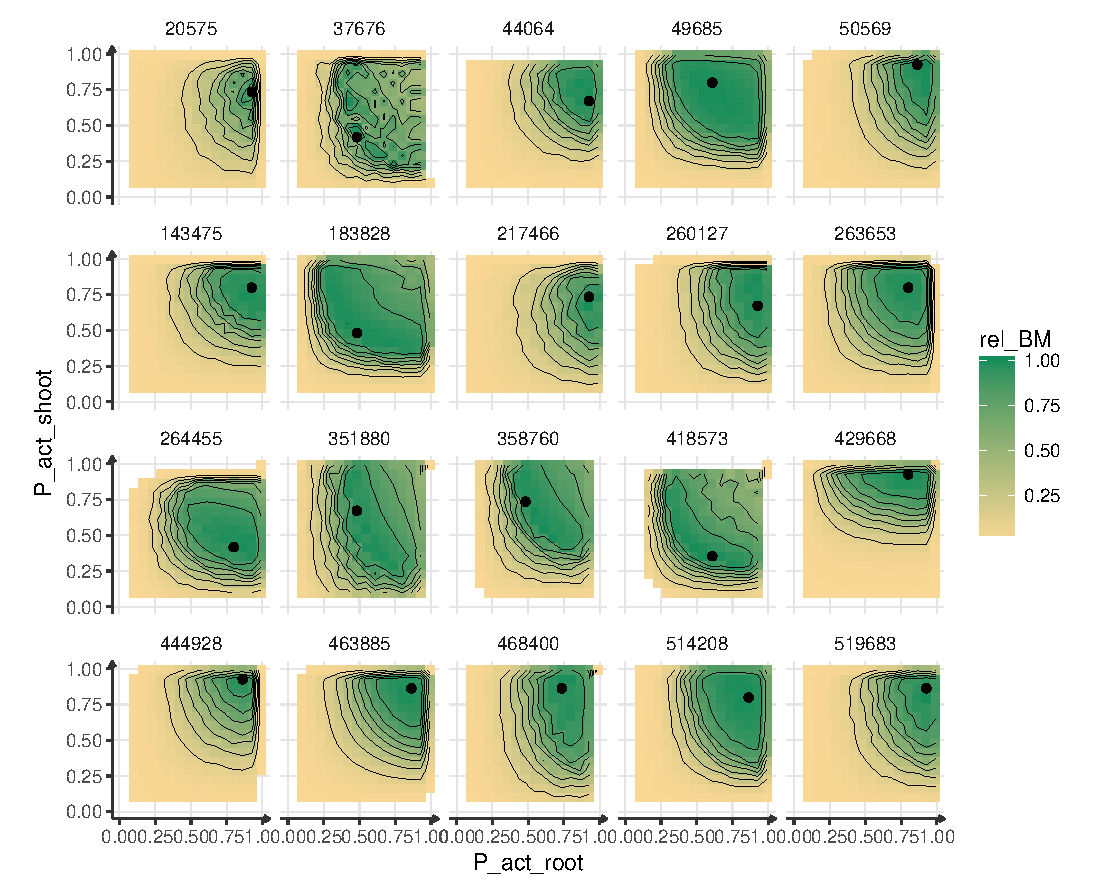
\includegraphics[width = \textwidth]{./2_PP/Figures/Landscape/landscape_PAR-PAS.pdf}
\caption{Projection of best phenotypes (varying RMF) on the 2D PAR-PAS plane for each parameter set. Points identify the optimums. \textit{Non plastic}.}
\end{figure}

 On the tissue allocation plan (proportion of active tissues in leaves and roots) (see figure \ref{fig:best_phenotypes}), the best performing phenotypes present a bean shape. This shape covers a good fraction of the space, in the center and sometimes top-right corner (high active tissue allocation) of the 2D space, while other corners are ignored. Too low values for any of the organs lead to a limited growth. For certain parameter sets, the top-right corner, corresponding to high resource acquisition strategies, has lower growth values than the center. They have lower growth values than phenotypes with similar values for one of the organ and lower value for the other organ.  %This shape suggest that relative importance of organ efficiency is lower than other criterion such as equilibrium and overall performance (see section \ref{chapter:modelling_PP} paragraph \ref{subsection:match} for the discussion on the components of plant performance). On this plane, the lowest values of plant biomass are characterised by low values of active tissue allocation. 
 

Projection of the best phenotypes over the three planes also gives information on the importance of the ignored variable on each plane. If the contrast between the growth projected phenotypes is high, at least on the main dimension is crucial for the growth. If the contrast is lower when the variable is ignored (\textit{i.e.} the best value is used) then the projected variable is likely to be important. The projection on PAR-RMF and PAS-RMF (see figure \ref{fig:projections}) planes show higher contrast between phenotypes relatively to PAR-PAS plane, therefore the RMF is a more sensitive variable than the allocation factors to active tissues in organs.


%Higher resource: contraction of the landscape, toward faster species. Moving optimum and moving gravity center. Transition to optimum shifting and difference between allocation rules.

\paragraph{Optimum shifting}

Introducing resource availability variations and plasticity can impact the shape of the performance landscape.

A shift of gravity centres can be observed between the two resource levels in all allocation algorithms (see figure \ref{fig:gravity_shift_resource}, the four panels). \textit{Non plastic} and \textit{fixed} algorithm show similar trends with an increase of proportion in active tissues in both organs. This change toward more exploitative tissues is consistent and is observable for all parameter sets but one. The \textit{plastic-optimisation} algorithm show drastically different responses of gravity center of phenotypes. There is little change in shoot proportion of active tissues, but a consistent reduction of active tissues in root system, and a reduction of root mass fraction (data not shown). These two responses indicates a net reduction of root activity in favour of shoot activity. Two things must be taken into consideration while looking at theese results: (1) the gravity center is computed from final position into the phenotypic space, not the starting position, (2) because \textit{plastic-optimisation} algorithm allows changes in traits that are represented (PAR and PAS), shifts along these axis can be driven by the plasticity mechanisms and not neceseraly only performance differences. Similar representation of the gravity center computed from the initial phenotype (not shown) shows similar response for the three first algorithms, and no apparent shift for the \textit{plastic-optimisation} plasticity.

\begin{figure}\label{fig:gravity_shift_resource}
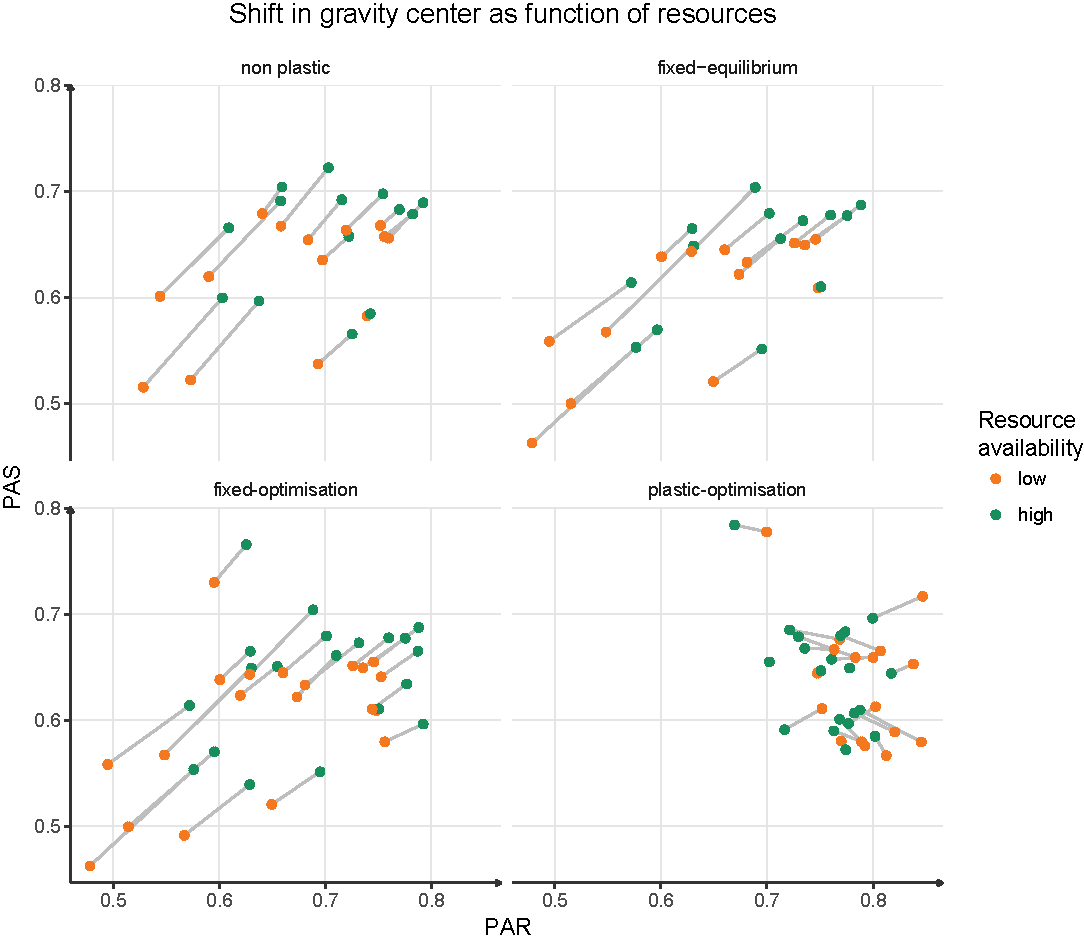
\includegraphics[width = \textwidth]{./2_PP/Figures/Landscape/ld_gravity_resourceall.pdf}
\caption{Shift on the 2D phenotypic space of the center of gravity as function of resource availability. The center of gravity is defined as the average phenotype weihted by the relative biomass, and characterises the performance landscape. \textit{Non plastic}.}
\end{figure}

\textit{Non plastic} and \textit{fixed} plasticities respond the same way to a shift in resource availability. However, we can note that the gravity centres have lower proportion of active tissues for \textit{fixed} allocation algorithm compared to the \textit{non plastic} one.

%
%Shift due to plasticity -- timing only ?
%+ shift (not fully significant in high resource availability) toward more exploit shoot and less exploit root. What does that mean ? higher tissue efficiency authorized by less limiting water ?
%
%Where is the optimum ?  what makes an optimum ? Why is it important ? -- beter understand how plasticity works and can improve plant performance.
%
%What are the sensitive dimensions ? and why ? 
%
%then moving optimum and why ?
%
%Moving optimum 2D: why ?
%
%What is the plastic-optimisation doing ? Wrong phenotype ? Wrong projection ? Wrong strategy or wrong RMF ? 

%\paragraph{Phenotypic space contraction}
\paragraph{Productivity changes}

Plastic allocation lead to an improvement in mean biomass of all individuals for all three plastic allocation algorithms (see figure \ref{fig:mean_BM_pl}). The \textit{fixed-equilibrium} plants are 2.5 times bigger in average than \textit{non plastic} plants (in low resource conditions, and up to 7 times bigger for \textit{plastic-optimisation} plant. These ratios are relatively similar for high resource availability. 

\begin{figure}\label{fig:mean_BM_pl}
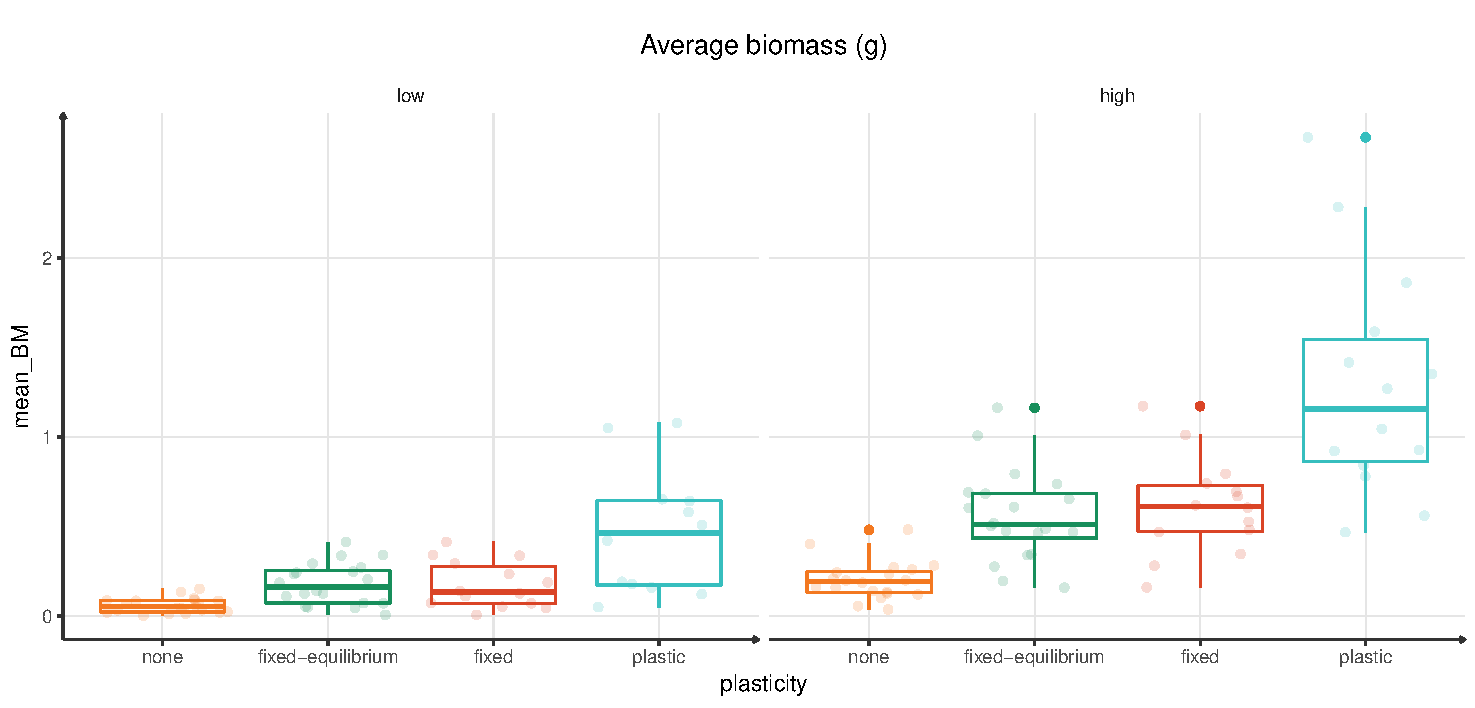
\includegraphics[width = \textwidth]{./2_PP/Figures/Landscape/plot_BM_allocation.pdf}
\caption{Mean relative biomass as a function of allocation algorithm and resource level.}
\end{figure}

However, the maximum biomass is only marginally improved with an increase of 6\% for \textit{fixed-equilibrium} and 8\% for \textit{fixed-optimisation} in low resource condition (see figure \ref{fig:max_BM_pl}). These percentages drop to less than 1\% in high resource availability conditions. The \textit{plastic-optimisation} algorithm even lead to a decrease in the maximum biomass averaging 10\% and 13\% respectively in low and high resource availability conditions.

\begin{figure}\label{fig:max_BM_pl}
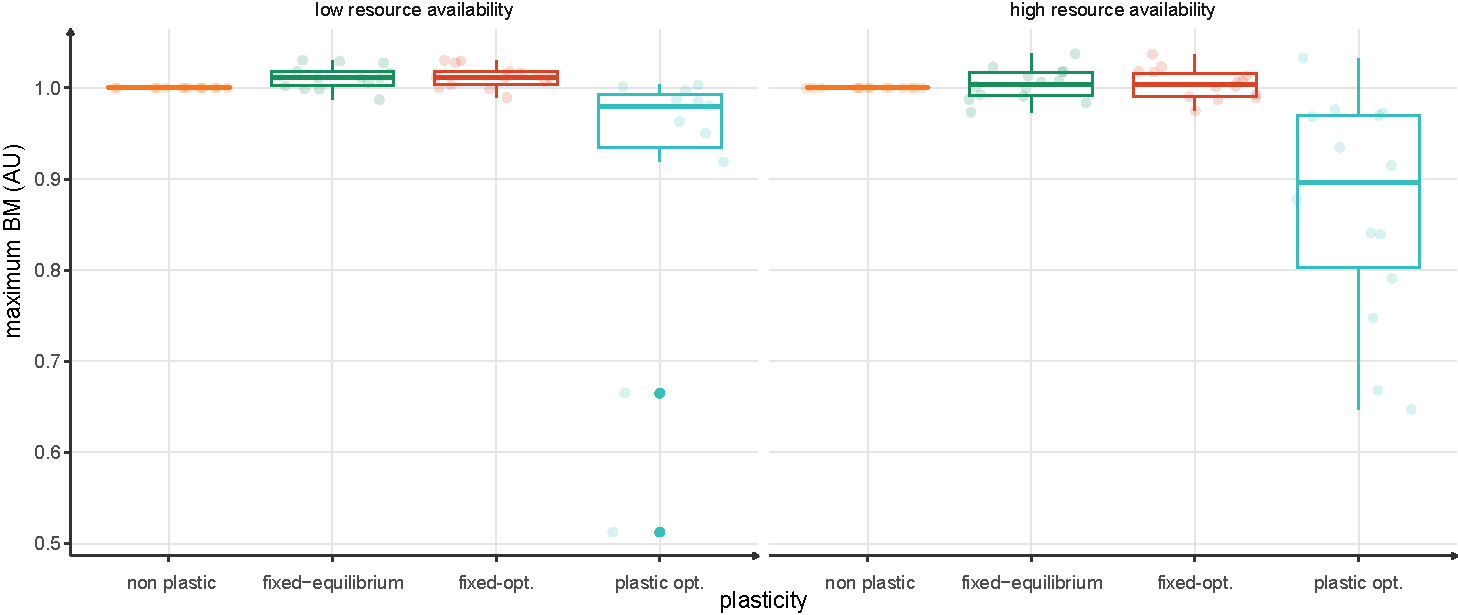
\includegraphics[width = \textwidth]{./2_PP/Figures/Landscape/plot_maxBM_allocation.pdf}
\caption{Maximum biomass relative to the \textit{non plastic} simulations, as a function of allocation algorithm and resource level.}
\end{figure}

\paragraph{Phenotypic convergence}

The effect of plasticity on the potential diversity is estimated by looking at the species that reach the range of 90\% to 100\% of the maximum biomass within the specific conditions (for each parameter set, algorithm and condition separately).

\begin{figure}\label{fig:species_richness}
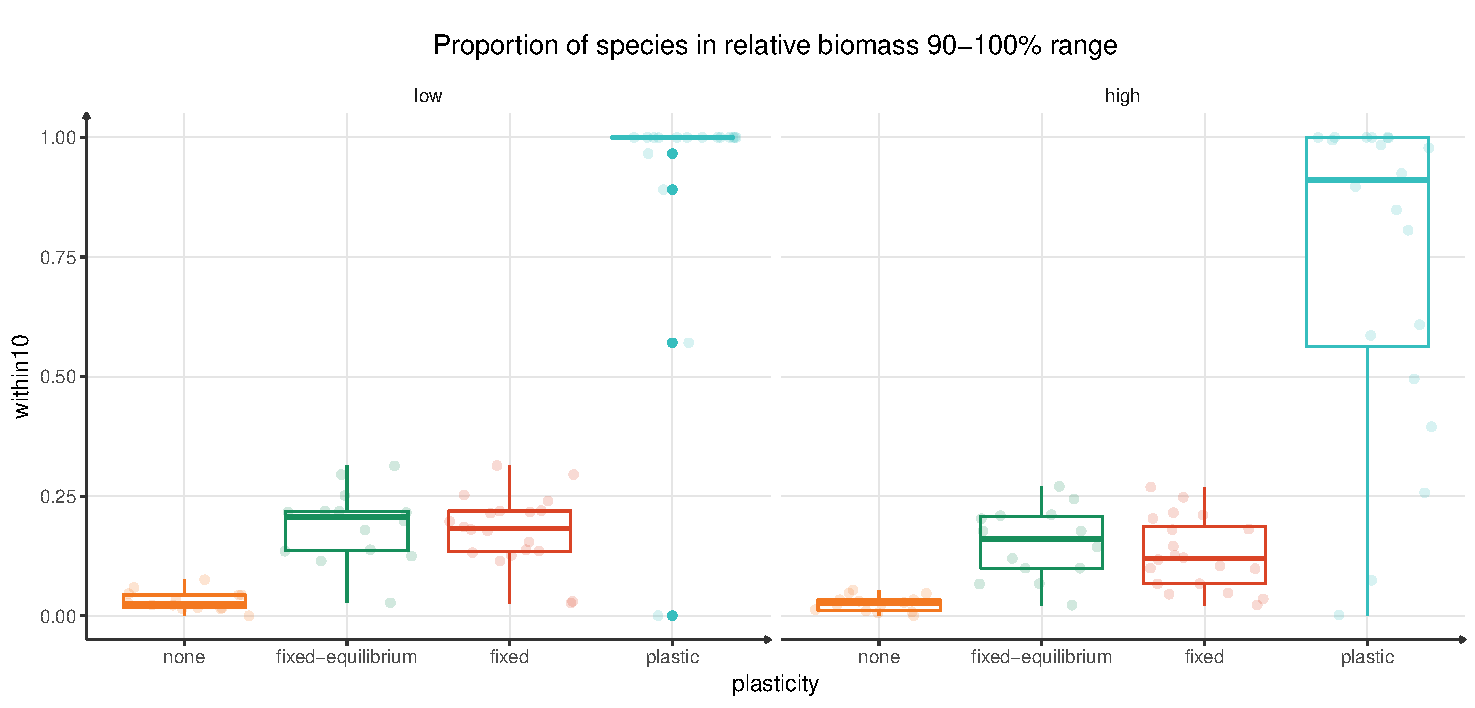
\includegraphics[width = \textwidth]{./2_PP/Figures/Landscape/plot_eveness.pdf}
\caption{Number of species within the range of 90\% to 100\% of the maximum biomass, as a function of allocation algorithm and resource level.}
\end{figure}

The number of species within this range is extremely low in \textit{non plastic} allocation algorithm simulations, with 1.4\% and 2.1\% respectively for low and high resource conditions. This percentage is greatly improved by plastic allocation algorithm and reach in average 9\% to 15\% of species in \textit{fixed-equilibrium} and \textit{fixed-optimisation} algorithm, while in can reach up to 100 \% for \textit{plastic-optimisation} algorithm, with a mean proportion of species with a top performance around 72\% in low availability condition, and up to 82\% in high resource availability condition.

\begin{figure}\label{fig:function_div}
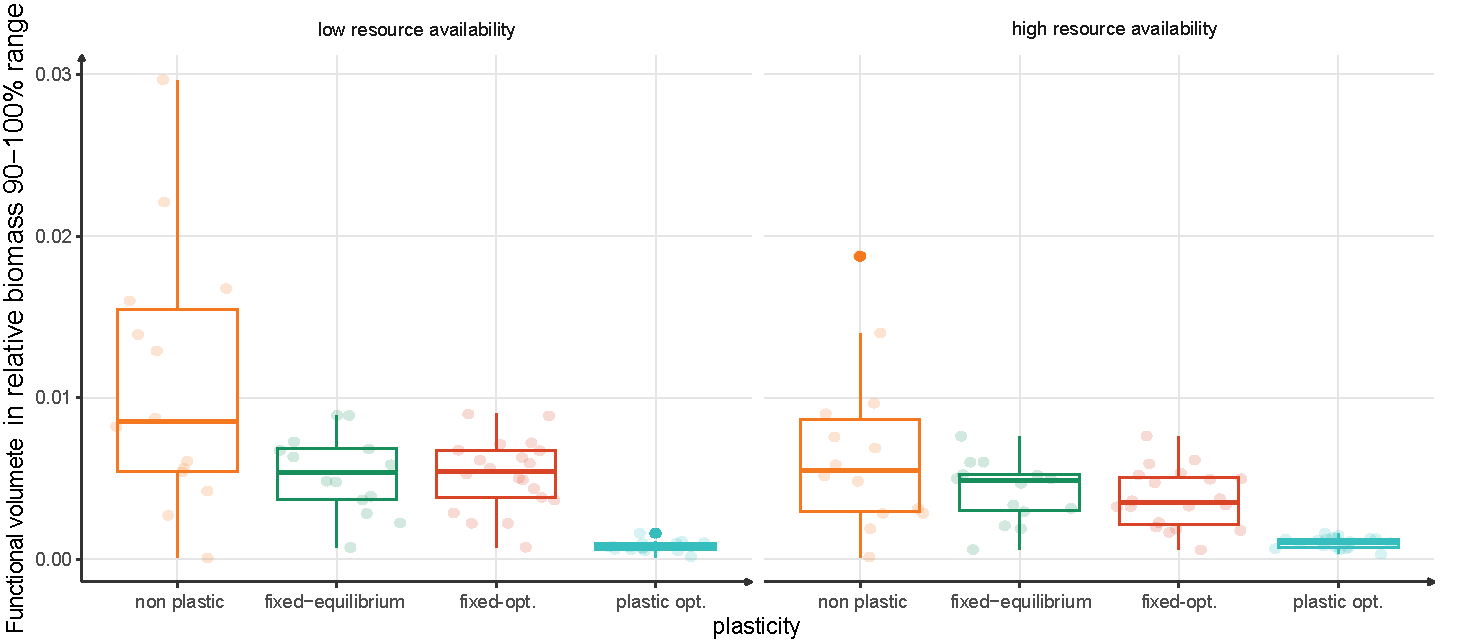
\includegraphics[width = \textwidth]{./2_PP/Figures/Landscape/plot_fdiv.pdf}
\caption{Functional volume occupied by the species within the range of 90\% to 100\% of the maximum biomass, as a function of allocation algorithm and resource level.}
\end{figure}

The functional diversity, estimated with the approximate volume of the top phenotypes, follows a opposite trend, with the highest value for the \textit{non plastic} allocation algorithm. \textit{Fixed} algorithms present half the functional volume of the \textit{non plastic} algorithm, and hte \textit{plastic-optimisation} algorithm has extremely low values five times lower than the \textit{non plastic} ones.



\subsection{Discussion}

\paragraph{Components of performance}

The study of the performance landscape puts in light the different components of \textemph{plant performance}. To understand how plasticity can play a role, it is important to understand what make a phenotype a good phenotype. 
% the main axis: 
On one hand, the extend of strategies (plan PAR-PAS in figure \ref{fig:best_phenotypes}) with high relative growth (green area) is high when the best  RMF is considered, while this is greatly reduced on plans that integrates RMF variability (see figure \ref{fig:perf_decomposition}). This result suggest the high importance on this axis for the plants performance. This can be explained by a stronger effect of this dimension on the exchange area through changes in organ masses, instead of organ densities (affected by PAR and PAS). The RMF fraction impacts the plant performance in two ways: by changing the \textemph{equilibrium} between shoot and root exchange activities, and by changing the global carbon loss rate (respiration and tissue turn-over) if the organ differ on this aspect. These two components may have opposed directions, as the limiting organ may also be the least efficient, and therefore the RMF could be greatly constrained if the two aspects have similar importance. The effect on the equilibrium is likely be more important as a wide range of RMF values can be observed for numerous datasets (data not shown), and plant with uncoordinated (low-PAS \& high-PAR, or high-PAS \& low-PAR, \see figure \ref{fig:perf_decomposition}) organs still present high biomass values, suggesting that the respiration and turn-over loss are less important than a balanced resource acquisition. 

%NEED THE DECOMPOSITION OF PLANT PERFORMANCE HERE

\begin{figure}%[tb]
    \classiccaptionstyle
\sidebysidecaption{0.60\textwidth}{0.3\textwidth}{%
    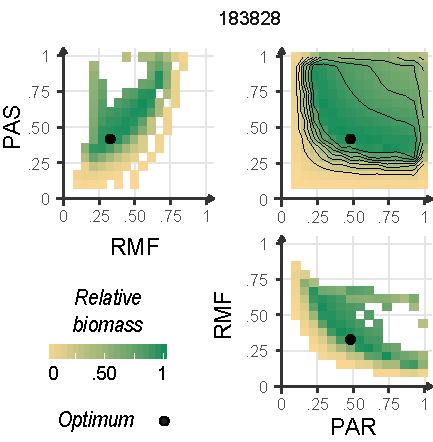
\includegraphics[width=1\linewidth]{./2_PP/Figures/Landscape/ld_space_ex.pdf}%
}{
  \caption[Projection of performance on phenotypic plans]{Projection for the parameter set 183828 of best phenotypes (according to the variable that is ignored) on 2D plans of the phenotypic space. The dots represent the optimum phenotype. White space indicates the absence of phenotypes able to survive until the end of the simulation (100 days). RMF: root mass fraction, PAR: proportion of active tissues in roots, PAS: proportion of active tissues in shoot. }
  \label{fig:perf_decomposition}
  }
\end{figure}

On the other hand the organ specific strategies are also important as low values for any of the organs (leaves or roots) lead to very low growth. Extreme high values can also be limiting, suggesting the existence of an optimum of the proportion of active tissue for the tissue efficient. This \textemph{optimum tissue efficiency} results from trade-off between active and structural tissues, driven by the relative importance of carbon gain (increased exchange area with active tissues) and carbon loss (increased respiration and turn-over with proportion of active tissues) that depends on models parameters and resource availability (that change the exchange rate).

\begin{marginfigure}\label{fig:function_div}
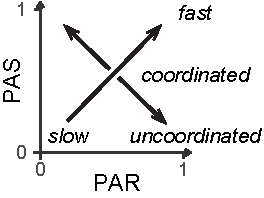
\includegraphics[width = \textwidth]{./2_PP/Figures/Landscape/ld_axis.pdf}
\caption{Alternative axes to describe the plant phenotypes on the plan PAR-PAR (PAR: proportion of active tissues in roots, PAS: proportion of active tissues in shoot). The slow-fast axis refers to the proportion of active tissues (close to the fast-slow strategies of \cite{reich_world-wide_2014}), while the orthogonal axis show how coordinated the plant is (see \cite{freschet_integrated_2015} for similar concept).}
\end{marginfigure}

However, meeting these tissues specific optima might not be sufficient, as the bean shape of the best phenotypes suggests, another component is relevant. Low values of proportion of active tissue in one organ can be compensated by a high allocation of active tissues in the other organ that allows a higher allocation in the low exchange rate organ. This confirms the importance of the equilibrium over the tissue specific strategies. But the shape also reveals a last component of the plant performances. The fact that species with high values of proportion of active tissues in both organs have lower biomass, is certainly due to a limitation of both resources (equilibrium is assumed), reducing the overall efficiency. 

From this visualisation of plant biomass as a function of the phenotypes, three main components play a role. The \textemph{equilibrium}, mostly driven by the changes in RMF is essential to the plant growth. This is explained by a reduction of the exchange rate of the non limiting organ that greatly reduces its organ specific efficiency (see figure \ref{fig:efficiency}). This \textemph{organ tissue efficiency}, driven by its effective exchange rate, respiration and turn-over, is also an important component of plant performance. Low values of allocation of active tissues greatly reduces this efficiency, but it can be compensated by bigger organs. However, such mechanisms can affect the overall efficiency defined as the average mean of organ realised efficiencies (taking into account resource limitations) weighted by the organ masses. Finally, the \textemph{speed} of the plant, or the overall resource acquisition rate, admits an optimum that is between an over-capacity leading to a co-limitation of resource on both organ reducing their individual efficiencies, and the under-capacity, leading to a sub-optimum use of resources and letting space for competition.

%NEED FIGURE OF EFFICIENCY: 

% the coordination

% the speed

%If equilibrium is a driving mechanisms in plant performance, for any given strategy (PAR-PAS plan projection) the best phenotypes has a RMF values that guarantee the functional equilibrium. However, for each strategy there is a notable difference between the RMF of best phenotypes  and the RMF of phenotypes the closest to the equilibrium. This disparity is positively related to the strategy balance: best phenotypes with higher active allocation in shoot than root have lower allocation to roots than required for functional equilibrium. 


%%\textemph{equilibrium}, overall \textemph{speed} and overall \textemph{efficiency}.\\
%The main thing with equilibrium is the total resource use.
%
%Better too fast than not fast enough.
%
%Explain the memory stuff in previous section: low-low compared to low-high, the second one lead to overall higher productivity (lack of one resource compensated by higher allocation to the related organ) that can support more active tissues. 
%
%The role of RMF: controlling variable, more sensitive than PAR and PAR but because bigger impact on balance: wide range on RMF values with similar performance: RMF value in itself is not that important: equilibrium is.
%
%Shifts in optimum, is it because plasticity provide more efficient functioning supporting more exploitative strategies, or side result from convergence that do not contain the previous optimum ?
%
%Convergence, relative species diversity and functional diversity.

\paragraph{Convergence to subspace}

The phenotypic plasticity allows species to move within this performance landscape along certain axis. It is is often perceived with a species-centric perspective, that is to say, that plasticity is seen as variations in the species mean phenotype. However, in the context of community ecology, it is also interesting to try to see how it not only affect individual species but shape the community distribution in the strategy space. The plasticity relies on changes of default phenotypes toward "better" strategies in the context of the given conditions, therefore it implies that if it exists an optimum subspace (one strategy or an ensemble of strategies) species will converge toward this subspace, distorting the functional space. Environmental variations and plant interactions aside, in a constant environment the \textemph{performance landscape} is fixed. As a consequence, the plasticity benefits to the plant in a static manner, that is to say, it is only a tool to reach a better phenotype where the plant stays in if conditions do not change. This can be related to spatial heterogeneity that would lead individuals from the same species to adopt different phenotype to acclimate to the particular conditions of their spatial situation. It is opposed to the perception of a more dynamic phenotypic plasticity as a tool for a given individual to cope with temporal variations in environmental conditions. These two aspects are further discussed in the following section, while the effects of the contraction of the phenotypic space are discussed now.

\begin{figure}\label{fig:convergence}
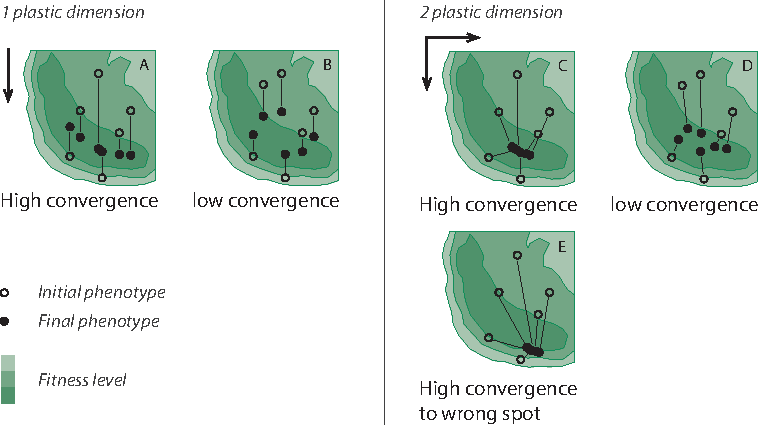
\includegraphics[width = \textwidth]{./2_PP/Figures/Landscape/ld_convergence.pdf}
\caption[Convergence patterns]{Convergence patterns on a 2D phenotypic fitness landscape, with 1 plastic dimension (A \& B) or 2 plastic dimensions (C, D \& E). Plasticity can lead to high convergence (A, C and E) with potentially high fitness evenness, especially in space with numerous plastic dimensions (A \& E), this is problematic especially if the point of convergence is not the optimum (E). Limits to high convergence are necessary to allow realistic functional diversity with plasticity (B \& D).}
\end{figure}

As just mentioned, the plasticity can be seen at the scale of the species assembly \sidenote{here I draw a distinction between species assembly that refers to all present species, and community that refers to the interacting individuals of the present species. However, some interpretations can be translated to communities.} as a contraction of the phenotypic space of the species assembly. This contraction has two main effects: the reduction of potential functional diversity and a reduction of growth rate differences. There is here an emerging trade-off between the \textemph{species diversity}, supported by lower fitness differences, and \textemph{functional diversity}, reduced by the contraction of the phenotypic space. However, if the plasticity reduces greatly the potential functional diversity (volume of the whole phenotypic space without considering filtering based on relative fitness), the realised diversity (expressed as the functional diversity of the species within the 90\%-100\% maximum biomass range) is less impacted because a large parts of the phenotypic space have low growth rate in the given conditions. Nevertheless, there is a reduction of the diversity of expressed phenotypes. Indeed, in this scenario of "extreme" plasticity ($\tau = 0$) the convergence is important on plastic dimensions while partial convergence would be enough to have good fitness (see conceptual figure \ref{fig:convergence}). Lower convergence on plastic dimension should lead to less compact phenotypic subspace while keeping relative fitness evenness. In the case of \textit{fixed-equilibrium} and \textit{fixed-optimisation} allocation mechanisms, this reduction of diversity is lower because only one axis is plastic.

A reduction of the phenotypic convergence can be achieved by other allocation mechanisms, differences in projection (different $\tau$ values leading to different projections) and plasticity costs. In heterogeneous system, this convergence is expected to be lower as heterogeneity will lead to different projections. The constraints imposed by fixed traits also reduce the risk of convergence (lower convergence in panel A than in panel C in figure \ref{fig:convergence}), and other dimensions than the 3 studied here can be involved in the definition of the optimum (chemical traits for example) lead to larger optimum sub-space.


\paragraph{On diversity}

The question of diversity is essential in ecology, it often refers to species richness, or different indexes to measure this richness. In the context of the ecosystem functioning and service, the functional diversity is often preferred to qualify the community. To measure the functional diversity, the selection of the measured traits has an importance then algorithms can be used, considering the relative species abundances or distances between measures \parencite{laliberte_distance-based_2010}. Here, in the context of simulations with species diverging only of the 3 vegetative phenotypic axes, the functional diversity is expressed an estimation of the functional volume occupied by the species with top performance within this 3D space. But, because under certain allocation algorithms, some dimensions are plastic, it is difficult to study how plasticity impacts the functional diversity. The plasticity of an axis can lead to convergence and certainly reduce the potential functional diversity as only a subspace is considered. This is problematic in this context because there is a high convergence due to the specific implementation of the plasticity based on a shared gain function (equilibrium or growth-optimisation), but is certainly reduced if the algorithm allow contrasted responses (with response curves for example), or optimum phenotypes depending on the other traits as it is the case for \textit{fixed} algorithms (as opposed as the \textit{plastic-optimisation} algorithm). Because of this phenomenon of convergence, that cannot be totally avoided and is inherent in plasticity, the functional diversity should be considered in relation with the species diversity. The functional volume is reduced by a factor between 1 and 2, while the species richness is increased by a factor from 5 to 10 (see figures \ref{fig:function_div}, \& \ref{fig:species_richness}). While the ratio between functional and species diversity decreases in plastic conditions, the overall effect o ndiversity could be positive, especially if there are other traits (non considered here) correlated to the initial phenotype. 

%Cost and distance, sensitivity to environmental cues as solutions to this problem. 
\paragraph{Limited gain}

The convergence of the phenotypes to a sub-space of lower performance lead to an increase in the mean biomass (see figure \ref{fig:max_BM_pl}). However, the maximum biomass is only marginally improved in \textit{fixed} plastic allocation simulations, and reduced in \textit{plastic optimisation} allocation simulations. This two contrasted results, show different effects of plasticity. The light increase can be due to either a dynamic gain or a static gain. The \textemph{dynamic gain} can emerge because the plant growth affects the resource availability, changing the optimum phenotype, and allowing plastic plants to follow this chaanges during time. It could also result from a \textemph{static gain} because the phenotypic plasticity allow a better resolution in tested phenotypes (the plastic axis are continuous while the phenoytpic space sampling was discrete). The role of plasticity and dynamic gain is explored in the following sections with temporal resource heterogeneity.

The reduction of the maximum biomass highlight the difficulty to find the optimum phenotype. Because, the growth mechanisms are reproduced in an exact manner in the plasticity algorithm, this mismatch is certainly due to a difficulty to project the future of resource availability. Because of that, it is possible that the gain in maximum biomass, mentioned above, due to static or dynamic gain is greater than it appears. The particular case of mis-projection in \textit{plastic-optimisation} simulations is discussed in the following paragraph. 

\textbf{The phenotypic plasticity can lead to a certain degree of convergence, especially if the target phenotypes defined by the implementation of the plasticity are more condition-specific than species specific. While it can have strong effects on the functional diversity for the plastic traits, it also leads to high species richness due to a convergence toward a more performing subspace, and can potentially increase the total functional diversity if other traits are considered and the phenotypes more constrained. }

%Because of high convergence of \textit{plastic-optimisation}, no improvment of maximum biomass, but the \textit{fixed} alternative thanks to convergence limited to one phenotypic dimension (RMF) higher biomass: either higher resolution, or improvement due to \textemph{dynamic plasticity}. The role of dynamic plasticity benefit is explore in temporal variation simulations in the following section.


%Somehow I need to talk about the cost of being wrong. Can be observe in the delta heatmap on delta strat and delta w-ini: in this case there is less impact of being wrong of memory if you're good with strategy, because your not in different conditions...\\

%Potential effect on diversity: lower functional diversity, increase evenness. Leave highest fitness spot free. Why ? environmental cues or gain function ? Delta between projections ? \\

%Anyway, being good is stable conditions may useless if cannot survive or keep gain in other conditions. >> look along gradient if best species keep their rank.\\


\paragraph{Plastic exhaustion}

\textit{Plastic-optimisation} algorithm is characterised by a high convergence of the species within the phenotypic space, high mean biomass but maximum biomass lower than best \textit{non plastic} phenotype, and high potential species diversity. The convergence is expected and explained by the fact that all three traits are plastic and all species (for a given resource level) experience similar conditions leading to the computation of the same optimum. The absence of plasticity cost limiting the convergence leads to a phenotype concentration toward this optimum. This convergence explains both the high potential species diversity, as all species have very similar growth rate, and the relatively high mean biomass because only few species did not survive or had very little growth rate.

The fact that this plasticity does not translates into higher maximum biomass is surprising, especially considering the fact that RMF plasticity improves maximum biomass (see figure \ref{fig:mean_BM_pl}). Lag in adaptation is often identified as a limit of plasticity \parencite{dewitt_costs_1998, van_kleunen_constraints_2005}, nevertheless, in a constant resource influx experiment, and considering the high phenotypic flexibility of plants in \model, this explanation is unlikely. Another problem highlighted with plasticity is its adaptiveness. Evolutionary speaking, it is hard to imagine the emergence and maintenance of a plasticity mechanism (in a given context) if it is no adaptive. Yet, such process could be maladaptive in a new context. Because plasticity is not emerging, but imposed by the simulation set up, its adaptiveness can be interrogated. Here adaptiveness do not refer to a reduction of fitness due to plasticity, but to the capacity of the plastic mechanism to define an optimum (or at least better) phenotype. Plasticity as implemented in model has no explicit bias and all mechanisms involved in plant growth are simulated by the allocation algorithm. The sampling of phenotypes is random and could be source of uncertainty, but it is uniform and no consistent drift is likely to emerge from the noise introduced by such sampling. The last aspect of plasticity that can affect the adaptiveness of plasticity is the estimation of conditions. The estimation of conditions is based on resource levels experienced by the plant and by definition are exact, therefore the problem lies in the projection of these conditions and how they translate into resource uptake.


\begin{figure}\label{fig:exchange_volume_projection}
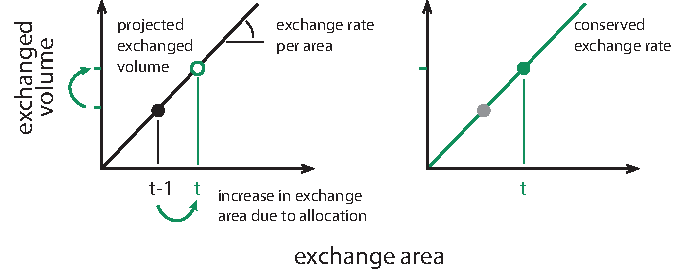
\includegraphics[width = \textwidth]{./2_PP/Figures/Concepts/exchange_volume_projection.pdf}
\caption{Projection of the water volume exchange after increase in exchange area at equilibrium and with no limitation.}
\end{figure}

In \model the resource availability is coded as an uptake rate per day and per unit of exchange area, and is computed as the resource uptake divided by the exchange area. This resource availability is supposed constant, and plants make the assumption that increasing their exchange area leads to a proportional increase in resource volume exchanged (see figure \ref{fig:exchange_volume_projection}).

\begin{figure}\label{fig:exhaustion}
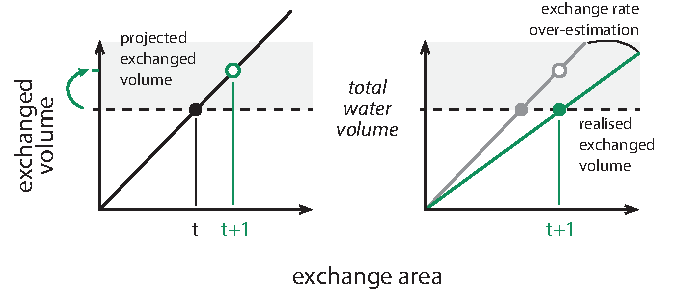
\includegraphics[width = \textwidth]{./2_PP/Figures/Concepts/exhaustion2.pdf}
\caption{Projection of the water volume exchange after increase in exchange area when total available water volume is limiting. The water volume exchanged cannot exceed the total available water volume, leading to a systematic over-estimation of water availability and offset between shoot and root activity.}
\end{figure}

However, in the case where a plant already absorbs all the available resource, then this assumption is not respected, and the uptake rate per area is lower than expected (see figure \ref{fig:exhaustion} right panel, realised exchanged volume does not match the projection because it cannot exceed the total volume of available water). This gap between perception and actual resource availability occurs because the plant is not able to perceive that the limitation cannot be compensated by a higher investment in the limiting organ. This behaviour explain a very high investment toward root and root active tissues in low resource conditions under \textit{plastic-optimisation} allocation (figure \ref{fig:gravity_shift_resource}). This gap\sidenote{this is different from a lag because it is not the result of slow changes in phenotype but comes from a default in the estimation of optimum phenotype.} is the cause of the \textemph{plastic exhaustion} phenomenon. Indeed, this constant over-estimation leads to constant discrepancy between the estimated optimum phenotype and the actual phenotype, and a larger allocation to root active tissues. This effect is particularly noticeable in the context of pot simulations where the water pool is limited. The absence of plasticity costs also favours such extreme behaviour. 

Despite this particular seemingly non-adaptive behaviour, the \textit{plastic-optimisation} algorithm is still interesting to study in community simulations. First, the presence of plasticity cost should limit such extreme behaviours. Second, in a context of competition in a larger environment, this aggressive search behaviour is likely to be an advantage against individual with less aggressive, or stable strategy. Finally, this mechanism emerges in constant influx conditions that allow growth, but its emergence should be reduced in variable environment where water shortage leads to reduced growth.

The plastic exhaustion mechanism seems to be contradictory with the previous observation that the proportion of active tissues does not increase when the related resource is limiting (see figure \ref{fig:memory_n_phenotype}), but it can be argued that it such extreme case, if the RMF has extreme values and is constrained by differences in tissue efficiencies. This is not verified however.

\textit{Plastic-optimisation} simulations expose this phenomenon with large effects, but it is probably present for simulations with other plastic allocations but with smaller effects. The difference in magnitude can be explained by a less effective growth in early stages of development for \textit{fixed} plasticities (when \textit{plastic-optimisation} is more efficient than fixed plasticities) that delay the time when the total volume is reached (time \textit{t} in figure \ref{fig:exhaustion}), and in average lower active tissue allocation in roots that leads to lower loss due to non-equilibrium.

\textbf{Plastic exhaustion is a specific limit of phenotypic plasticity as implemented in \model that relies on the assumption of constant exchange rate per exchange area. It has a large effect in the specific case of pot simulations. However, this phenomenon can be mitigated by plasticity cost linked to changes in traits, and can have adaptive value in a context of competition. Therefore, I argue that \textit{plastic-optimisation} algorithm  has low information value in the context of pot simulations with constant resource influx, but should still be studied in the context of community dynamics.}

%
%\paragraph{On diversity}
%Effects on diversity.\\ I would put that aside for now
%
%The potential functional diversity is amplified by the fact that many phenotypes that are not viable in any condition but becomes viable thanks to static gain of plasticity. These species exist in the context of the simulation because there is no cost to plasticity. Because species are uniformly sampled in the 3D, a lot of them could not grow in a lot of conditions ?

\paragraph{Resource availability}

%results from this part\\
As expected the resource availability and the resource balance are key components of the plant growth, to which the plant phenotype needs to match. Aside from the increase in biomass, an increase in "speed" of optimum phenotypes can result from higher resource availability. This observation is in agreement with empirical data that demonstrate higher SLA and faster physiology in favourable conditions. This aspect was less obvious in the response of species under \textit{plastic-optimisation} allocation that shifted more in term of balance and RMF. This may be due to a change in the relative balance between both resources as their availability (from the plant perspective) are linked to the global resource levels by non linear relationships.

The fact that plastic plants (for \textit{fixed} allocation algorithms) show shifts of optimum strategies toward more exploitative phenotypes, in addition to the \textit{non plastic} optimum shifts, in conditions of higher productivity demonstrate the importance of these strategies for the plant growth. However, the extend of this effect of conditions on optimum phenotype is susceptible to vary along a gradient. Indeed, because of the non linearity of relationships between resource levels and exchanges rates, and between exchange rates and growth rates, the link between the optimum phenotype and a resource gradient is likely to be non linear itself. In addition, phenotypic plasticity might also change the sensitivity of the phenotype to the resource level.

%Why we need to go for a gradient.

%\subsection{Extended discussion}
% level discussion}
%? about what ? Community dynamics ? pp impact of these dynamics ? coexistence of species

 

%Can functional diversity be measured for plastic tratis: different effects on plastic and non plastic traits ?


%\paragraph{Nuances around plasticity}
%This analysis was conduced with drastic parameters of plasticity with plastic plants relying only on their perception of external conditions to develop their phenotype. The different results ... different directions and impact on potential diversity.
%
%Also, some species may not benefit from plasticity, especially if it has a cost, while others can benefit a lot from plasticity.
%
%The contrasting responses of the different algorithms highlight the importance of the allocation mechanism. However, the unique framework implemented in \model creates a variety of nuanced responses that are not all explored here. But, the continuous gradient of strategy between species relying on species memory only and species following their perception of external condition should be kept in mind during the interpretation of these results and following.
%
%\textbf{Subsection conclusion: bla bla bla}

\textbf{The study of the performance landscape highlight the importance of the RMF phenotypic dimension to regulate the balance between shoot and root. In the other hand, the proportion of active tissues in the two compartments impacts the performance in a more subtle way with possibility of balance between the two organs thanks to the RMF. It also highlights the existence of a tight sub-space with higher performances, leading to high convergence under plastic allocation. This convergence can be problematic if the plasticity fails to be adaptive under specific circumstances. It can lead to a reduction of the functional diversity, but also increases the species diversity, altering the species-functional diversity relationship with potential consequences on the community functioning. The performance landscape is sensitive to the global resource availability, altering the relative fitness of species and their competitive relationships. This effect must be further studied to understand the link between the optimum phenotypes and the resource availability heterogeneity, and how plasticity can impact this link. }

% ##################################################################################
% ##################################################################################
% ##################################################################################


\section{Plasticity and variability of conditions}
%Question I try to answer: (use of schematics ?)
The heterogeneity of conditions is an essential mechanism for plant coexistence. Plasticity is likely to alter the effect of this heterogeneity on plant coexistence and relative performance. The impact of plasticity on this relationship between spatial and temporal \textemph{heterogeneity} of resources (here limited to water) and strategy dominance is explored with the model \model.\\

How does plasticity impact the performance of the different phenotype along a resource gradient? How can these potential changes affect the identity, diversity and productivity of mountain grassland communities?

%The phenotypic plasticity can impact the optimum strategy, but how does this effect impact the optimum phenotype along a resource availability gradient?
%Effect on optimum strategy: from previous conclusions and hypothesis to simulation method.\\

%Is the contraction effect on species richness, functional diversity and productivity changing along such gradient?
%Then on diversity: how good strategies perform when it is plastic. Pool of species that exist in different conditions to get rid of the static effect.

\subsection{Method}

Because the coordination is shown to be less important than the equilibrium, the below-ground resource acquisition is expected to be important in mountain grassland under climate change scenarios, and an extensive simulation plan comes with high computational cost, only root strategies are sampled and studied in this part. Considering the structure of the model, the conclusions about the root compartment can certainly be extended to the shoot compartment.

\paragraph{Simulation set-up}
For each of the 20 selected parameter sets, the growth of 400 plants (20 PAR values between 0.25 and 0.95, and 20 memory values between 0.1 and 1) is simulated for 100 days in square pots of 12 centimetres deep and 90 centimetres wide (to avoid quick self-competition) in a temperature of 20 degrees celsius during the day of 15 hours, and 10 degrees during the night. The radiance is set to the high values of 122 Watt per hour and per square metre. Because \textit{fixed} algorithms showed similar results, and the \textit{plastic-optimisation} algorithm show strange results, only two allocation algorithms are simulated: \textit{non plastic} and \textit{fixed-equilibrium}.

\paragraph{Spatial heterogeneity}
Spatial heterogeneity of water level is mimicked by a gradient of water influx. The growth of all 400 species described above are simulated for \textit{non plastic} and \textit{fixed-equilibrium} algorithm independently in separated simulations where the water influx is regularly sampled between 0.05 and 7 mm per day (20 values).

\paragraph{Temporal heterogeneity}
Similar set-up is used for temporal heterogeneity simulations. Because the range of water influx used in the previosus simulation is too wide, a lower value is chosen as the mean water influx. This value of 1.3mm per day corresponds to a point around which there is variations in the optimum strategies for most parameter sets. It is also relatively close to average rainfalls in the Alps during summer. 

\subsection{Results: gradient of homogeneous precipitation conditions}

\paragraph{Optimum strategy}

To study the effect of plasticity on community identity along a precipitation gradient, we can look at the position of the optimum strategy (PAR) along such gradient with different allocation algorithms.

%%Only look at the median of best strat. Gravity center lower for fixed-equilibrium, because of a few more species living.

The effect of allocation algorithm is observed on all species by plotting the position of the median \textit{optimum} along the watering gradient that translates what part of the strategy spectrum (from conservative to exploitative) benefit from the simulation conditions. At the low end of the gradient, conservative species exhibit higher growth than exploitative species with a median optimum around 25\% of active tissues in roots for both the \textit{non plastic}and the \textit{fixed-equilibrium} plastic allocation. In the other end of the spectrum, for watering values above 1 mm per day, the \textit{optimum} reaches a high point (median around 90\% of active tissues for both algorithms) demonstrating better performance of the exploitative species in high resource availability conditions.  There is not apparent differences between algorithms and the optimum is conserved along the gradient. There is a similar shift with an increase of optimum water availability memory for \textit{non plastic} algorithm.


\begin{figure}\label{fig:gradient_strat_trend}
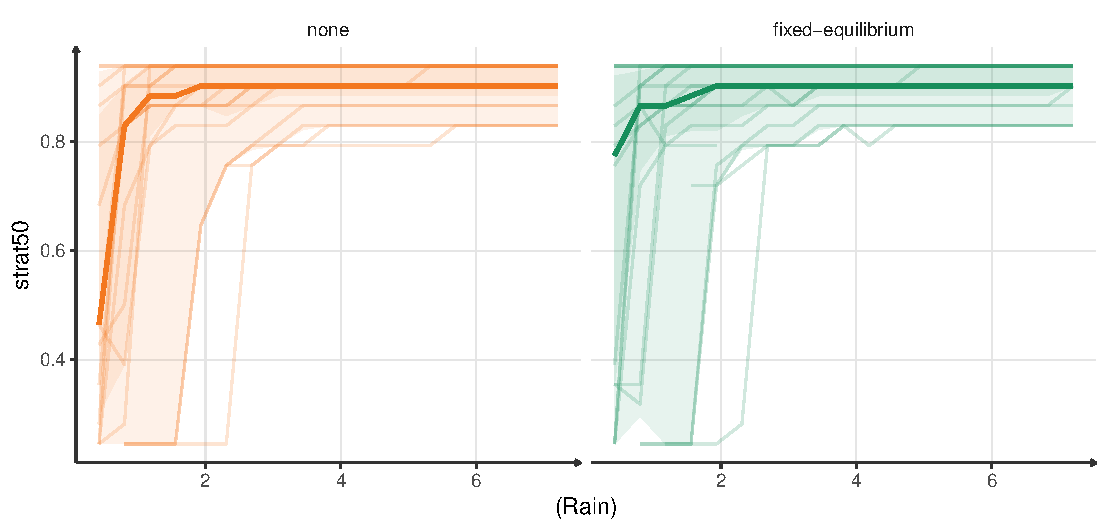
\includegraphics[width = \textwidth]{./2_PP/Figures/Rain/gradient_strat_trend.pdf}
\caption{Median (dark line \textbf{-}) optimum root strategy along the water treatment gradient for \textcolor{myOrange}{- \textit{non plastic}} \&  \textcolor{myGreen}{- \textit{fixed-equilibrium}} allocation algorithms. The light lines (-) correspond to the 20 independent parameter sets. The color ribbon marks the band between the 5th and 95th percentiles.} % Maybe I should change that so it is the 25th and 75th like for variable inputs.
\end{figure}

The memory of water availability of best performing phenotypes increases along the gradient under \textit{non plastic} allocation (see figure \ref{fig:gradient_w_ini_trend}, left panel), but the plasticity negates the effect of this species specific parameter and no lcear pattern can be observed (right panel).


\begin{figure}\label{fig:gradient_w_ini_trend}
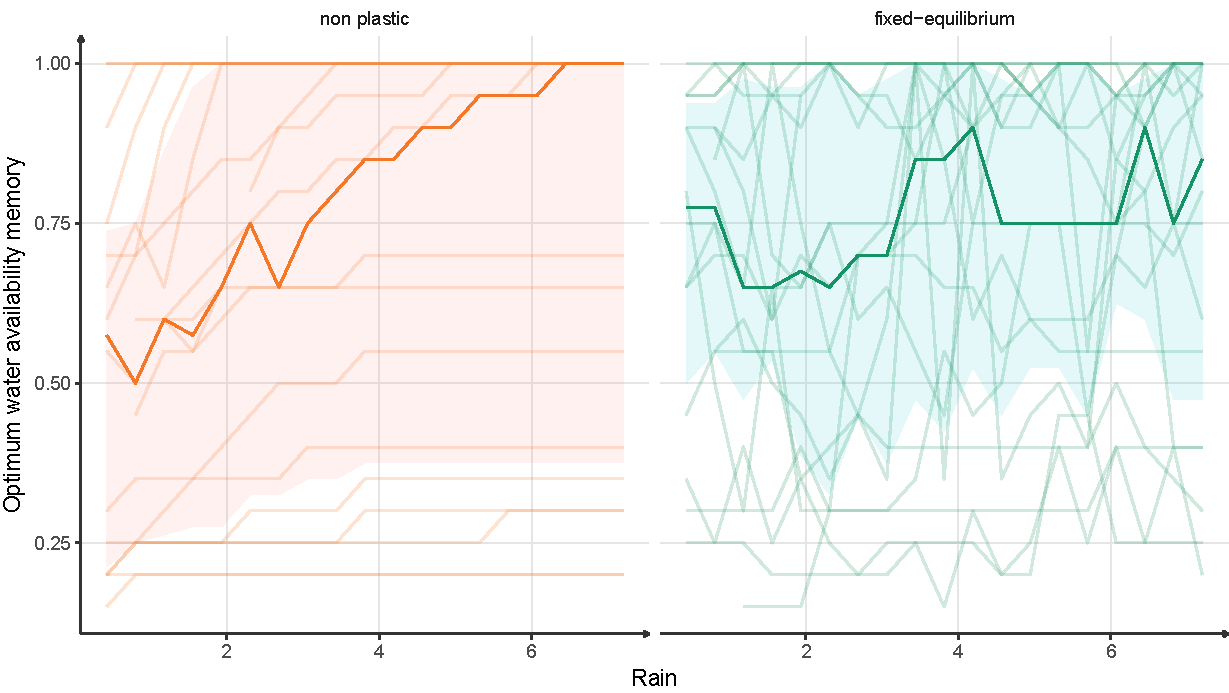
\includegraphics[width = \textwidth]{./2_PP/Figures/Rain/best_w_ini_pl_rain_grad_alt.pdf}
\caption{Median (dark line \textbf{-}) optimum water avaialbility memory along the water treatment gradient for \textcolor{myOrange}{- \textit{non plastic}} \&  \textcolor{myGreen}{- \textit{fixed-equilibrium}} allocation algorithms. The light lines (-) correspond to the 20 independent parameter sets. The color ribbon marks the band between the 5th and 95th percentiles.} % Maybe I should change that so it is the 25th and 75th like for variable inputs.
\end{figure}


\paragraph{Bigger productivity?}

The total cumulative biomass of all plants increases along the precipitation gradients. The plastic simulations have a cumulative biomass that is twice the biomass of \textit{non plastic} simulations.
%Strongly affect the potential overall productivity captured by cumulative biomass.


\begin{figure}\label{fig:total_BM}
    \classiccaptionstyle
\sidebysidecaption{0.60\textwidth}{0.3\textwidth}{%
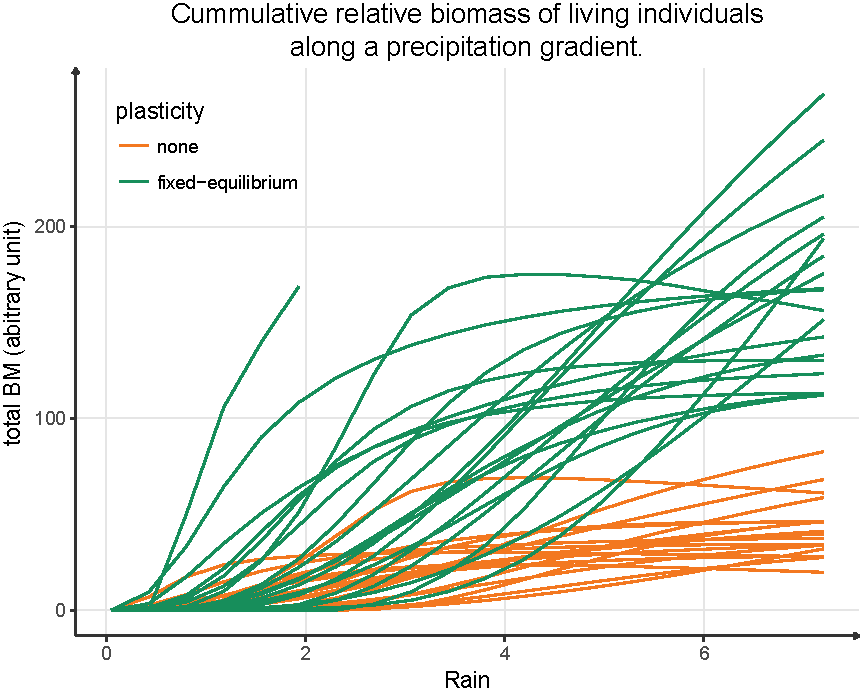
\includegraphics[width = \textwidth]{./2_PP/Figures/Rain/gradient_cumBM.pdf}
}{
\caption[Total biomass along a precipitation gradient]{Total biomass of all individual along a precipitation gradient for all tested parameter sets. Colour distinguishes plasticity treatments: \textcolor{myOrange}{- \textit{non plastic}} \&  \textcolor{myGreen}{- \textit{fixed-equilibrium}}.}
  }
\end{figure}

The effect on the maximum biomass is also investigated. For most simulation the maximum biomass is unchanged, and the median of the maximum biomass follow the same path for both conditions. However, the 75th and the 95th percentiles of plastic simulations shows a high increase in maximum biomass.
% But, only marginaly (for a few parameter sets) increases the biomass of best species.

\begin{figure}\label{fig:maximum_BM}
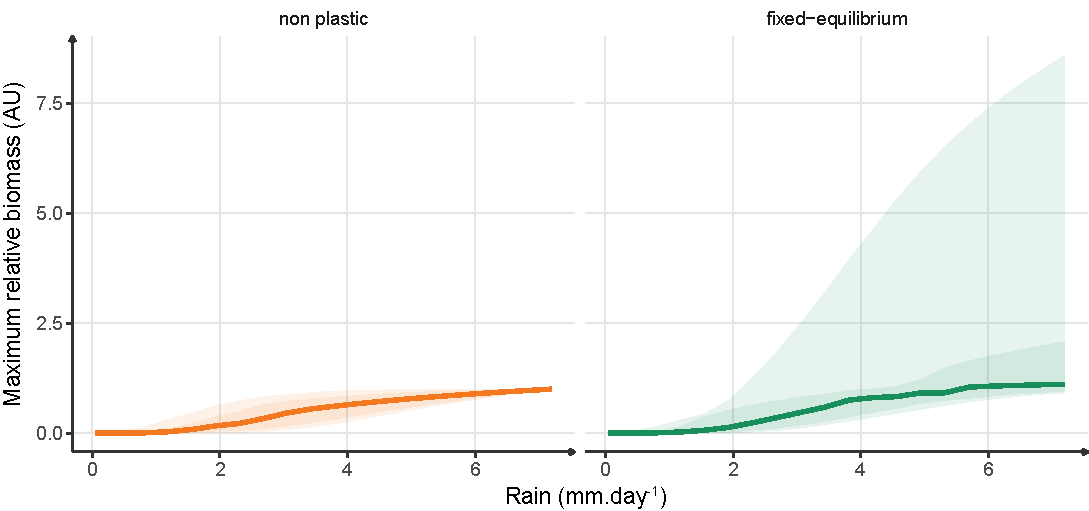
\includegraphics[width = \textwidth]{./2_PP/Figures/Rain/gradient_rel_BM_pl_trend.pdf}
\caption[Maximum biomass relative along a precipitation gradient]{Maximum biomass relative to the best performing plant in the most favourable condition for each parameter set, along a precipitation gradient.  Colour distinguishes plasticity treatments: \textcolor{myOrange}{- \textit{non plastic}} \&  \textcolor{myGreen}{- \textit{fixed-equilibrium}}.}
\end{figure}

%That probably means more species reaching high performance levels.

\paragraph{What about diversity?}

Similarly to the previous results, the potential diversity is estimated with the number of species, or the functional volume, of the species within the 90\%-100\% range of the maximum biomass for the given conditions.

\begin{figure}\label{fig:species_richness_grad}
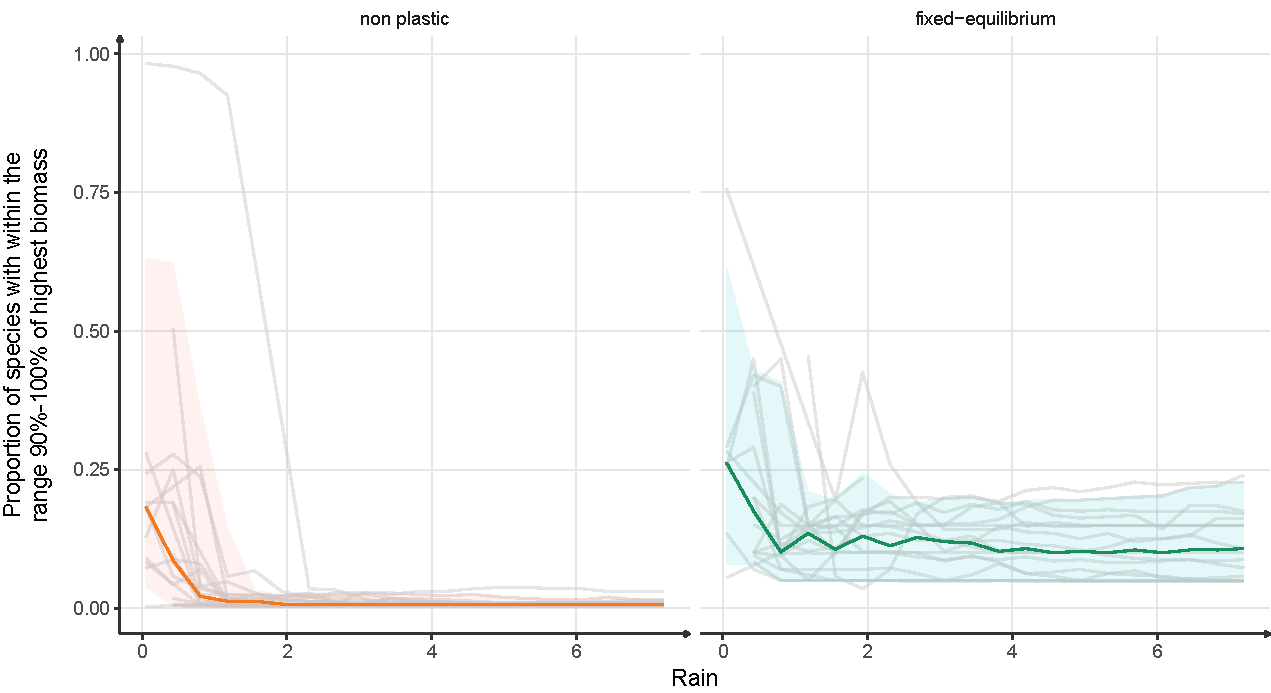
\includegraphics[width = \textwidth]{./2_PP/Figures/Rain/gradient_plot_spdiv10.pdf}
\caption[Species richness of the best performing species along a precipitation gradient]{Species richness of the species within the range 90\%-100\% of highest biomass for any given condition (parameter and precipitation) along a precipitation gradient.  Colour distinguishes plasticity treatments: \textcolor{myOrange}{- \textit{non plastic}} \&  \textcolor{myGreen}{- \textit{fixed-equilibrium}}.} \end{figure}

The species richness decreases along the gradient for the two plasticity treatments. The medians of species richness reach the low point for the same precipitation values than the medians of the optimum reach the highest values. The \textit{fixed-equilibrium} simulations show highest species richness along the whole gradient (except for one parameter set).

\begin{figure}\label{fig:functional_div_grad}
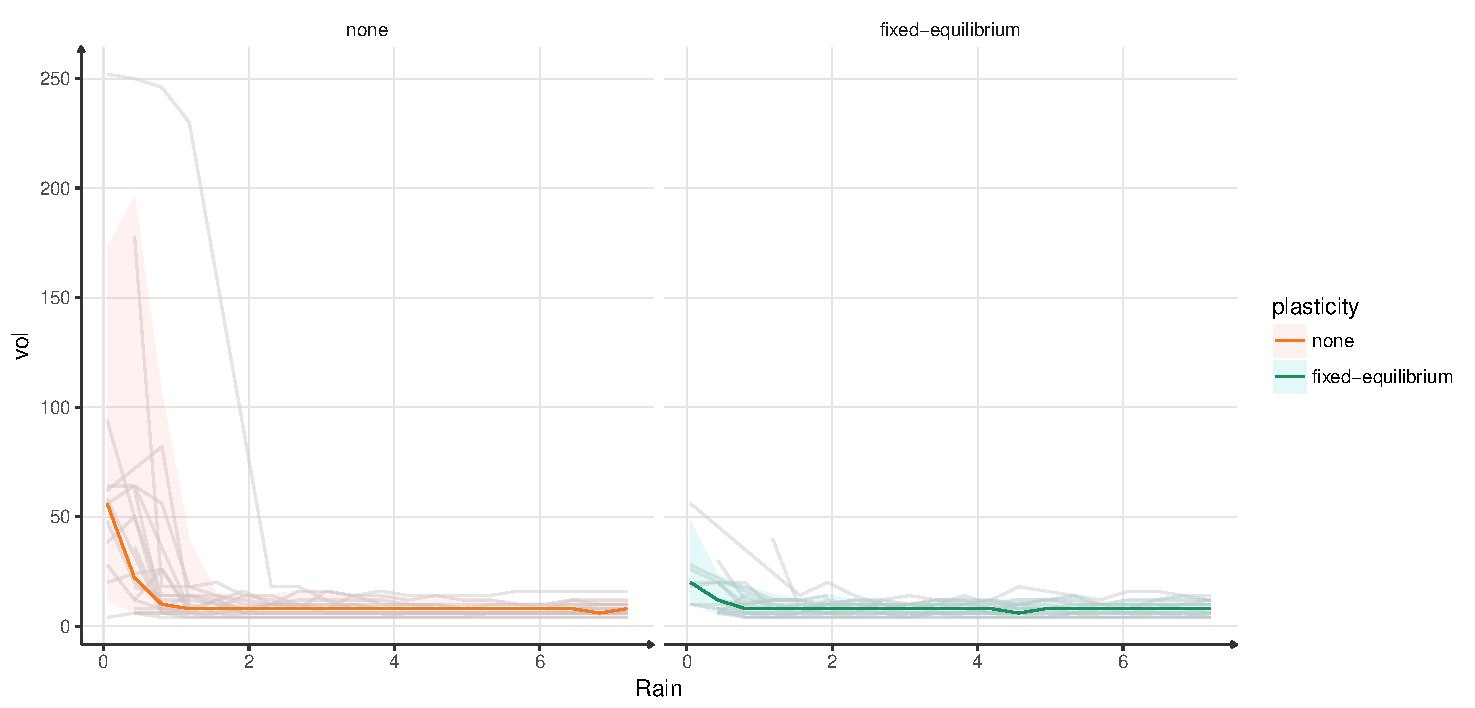
\includegraphics[width = \textwidth]{./2_PP/Figures/Rain/gradient_plot_fdiv10.pdf}
\caption[Functional diversity of the best performing species along a precipitation gradient]{Estimation of the functional volume occupied by the species within the range 90\%-100\% of highest biomass for any given condition (parameter and precipitation) along a precipitation gradient.  Colour distinguishes plasticity treatments: \textcolor{myOrange}{- \textit{non plastic}} \&  \textcolor{myGreen}{- \textit{fixed-equilibrium}}.} \end{figure}

The functional volume occupied by the top species, also decreases for both plasticity when the precipitations increase. For low watering values, the functional volume of \textit{non plastic} simulation is higher, however this difference disappear when both group of simulations reach low functional diversity.

\paragraph{Potential niches}

%A lot of effects discussed here emerge because a lot of different memories (equivalently RMF values) are associated to each resource use strategy for roots (shoot active tissue allocation being fixed and shared by all species). Another way of looking at the effect of plasticity focuses on only species identified as the best in at least one of the rain conditions. This focus reduces the number of species to species selected along such gradient and allow to ignore species that would not be present anyway. This selection does not take into account any competitive mechanisms that could change the identity of the dominant species in a given condition. Nevertheless, information on how the relative performance of theses species can still be collected.

%The potential effect of plasticity on niche breadth is visualised here for one representative parameter set.
The median performance of the best performing phenotypes for each conditions of the gradient are compared with and without RMF plasticity (\textit{fixed-equilibrium}) along the gradient. It is limited to the best phenotypes to mimic a degree of biotic filtering. The plasticity greatly enhance the ability of the plants to maintain a high growth, often comparable to the one of the best phenotype, along the gradient. The extreme low value of the gradient show no differences between phenotypes because the water level does not allow plant to grow, only the organic matter contain is the seed is used, leading to similar outputs. As seen in figure \ref{fig:gradient_strat_trend}, the best phenotypes often share the same strategy, but differ in memory for resource availability (figure \ref{fig:gradient_strat_trend}). Under \textit{fixed-equilibrium} allocation (right panel), the left end of the gradient (except the first value of precipitation) shows more contrast in the performances in strategies, while the righ end (more water) shows very little contrast. This is very different from the \textit{non plastic} allocation results (left panel) that show large differences between the best strategies along the whole gradient.  

\begin{figure}\label{fig:gradient_ranking}
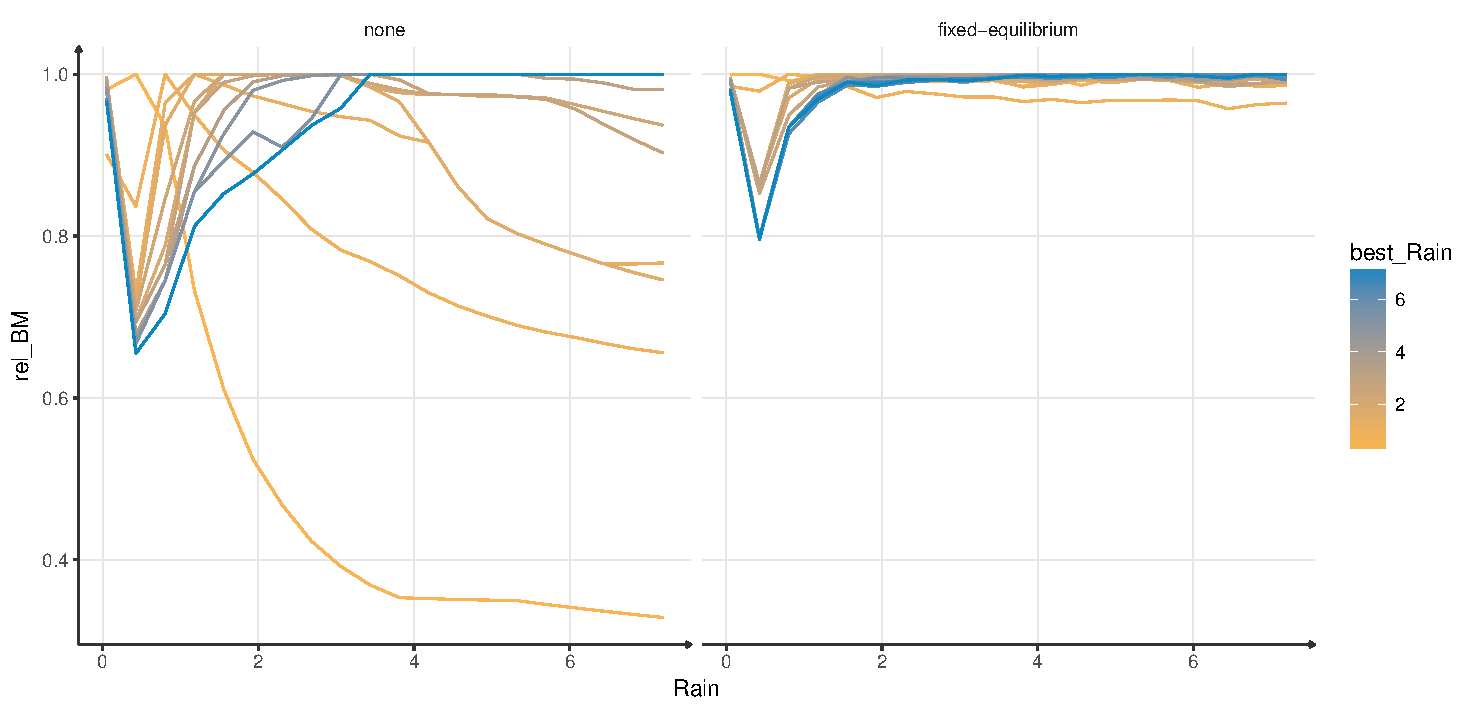
\includegraphics[width = \textwidth]{./2_PP/Figures/Rain/optimum_shifting_median.pdf}
\caption{Median relative performance of best phenotypes along a precipitation gradient for 20 parameter sets.}
\end{figure}

%The effect of the plasticity on the potential niche can be observed by looking at the cumulative number of species within the 91\%-100\% range of maximum biomass along the gradient (figure \ref{fig:gradient_ranges}). For all parameter sets, there is an increase in the number of species 
%
%
%\begin{figure}\label{fig:gradient_ranges}
%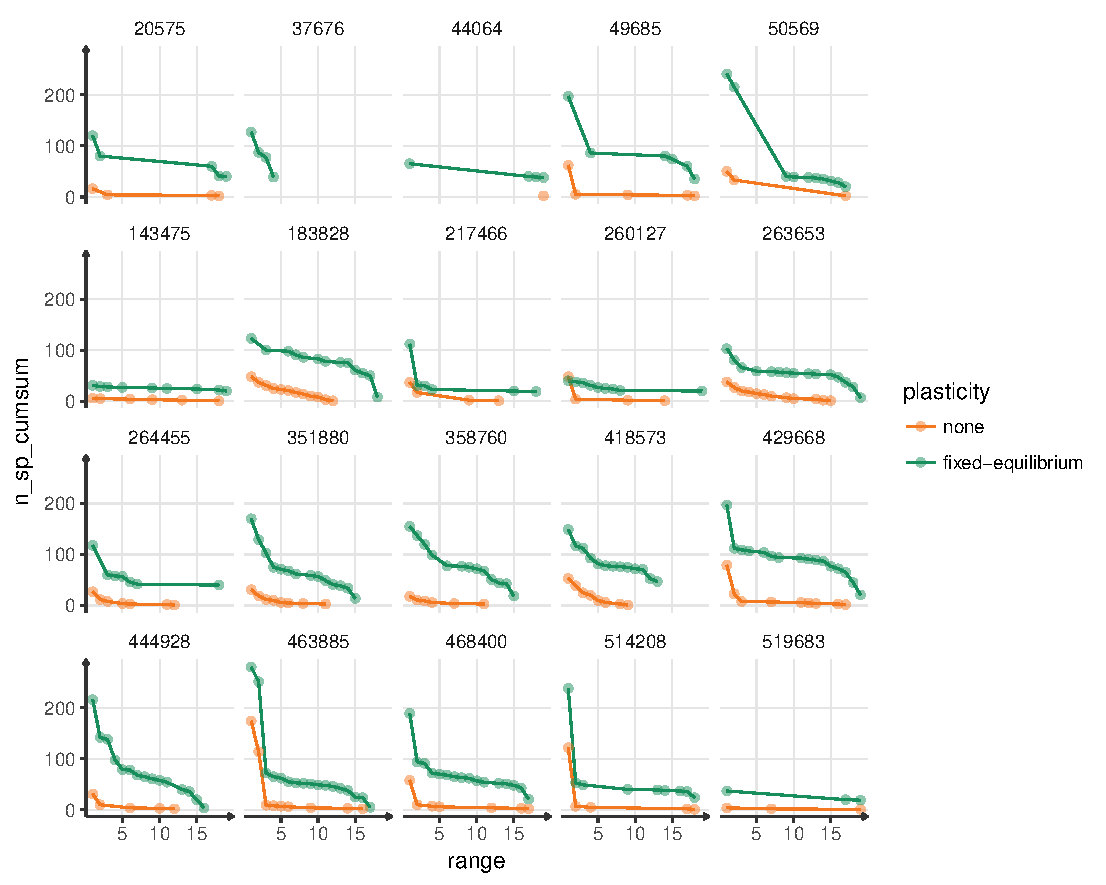
\includegraphics[width = \textwidth]{./2_PP/Figures/Rain/gradient_range_nb_sp.pdf}
%\caption[Changes the dominance structure]{Changes in the dominance structure for the evaluated parameter sets. The dominance structure is illustrated by the cumulative number of species along diminnishing number of conditions where they are within the top 90\%-100\% range of highest biomass for any given condition. }
%\end{figure}




\subsection{Discussion: gradient of homogeneous conditions}

\paragraph{Strategy shift}
Along the watering gradient, the \textemph{optimum strategy} (active tissue allocation in roots) changes from conservative toward exploitative. This shift demonstrates that the trade-off between active and structural tissues allocation allows different strategy to dominate in constrasting conditions \parencite{wright_worldwide_2006}. This shift occurs for low values of the gradient and exploitative strategies are dominant over a large part of this gradient. The shape of the relationship results from the gradient including high precipitation values. Also, the low resolution of the strategies (15 values for the proportion of active tissues in roots) limits the possible number of different dominant strategies along such gradient. Because we can see a wide range of optimum of resource-use strategies, and the relationship between this variable and the resource availability is certainly continuous, we can be confident in the pattern observed and a positive relationship between these two variables.

% a few words on the memory
The optimum memory also shows a shift, from low water availability memory in low water conditions, to high values in high water availability conditions. This response is less strong than for the optimum strategy certainly because the relationship is more linear. The fact that the plasticity negates this relationship confirms the role of this variable as a control on the RMF, control that is not longer useful under plastic allocation with no cost.

%Explain why there is shift
This shift in memory is trivial to understand as the memory of light availability is fixed and the ratio between light and water memory controls the RMF. An increase in the memory (for \textit{non plastic} plants) translates directly in a reduction of the RMF. The shift in optimum is less obvious, despite being described in the literature. The core of this trade-of is the trade-of between tissue efficiency and exchange rates. The more conservative species are more resource-efficient as they consume less resource to produce a bigger amount of organic matter, allowing them to be productive even in low resource conditions. On the other hand, exploitative species have a lower resource-efficiency but can exchange more resources thanks to high exchange rates per unit of biomass. This differences are illustrated in the figure \ref{fig:asymmetric_gain}, in high resource availability conditions (left panel) the exploitative species B show higher growth, despite having lower efficiency (costs relative to gain are higher), while its growth is lower when the gains are reduced linearly by a reduction of the exchange rate due to lower resource availability. 

\begin{figure}
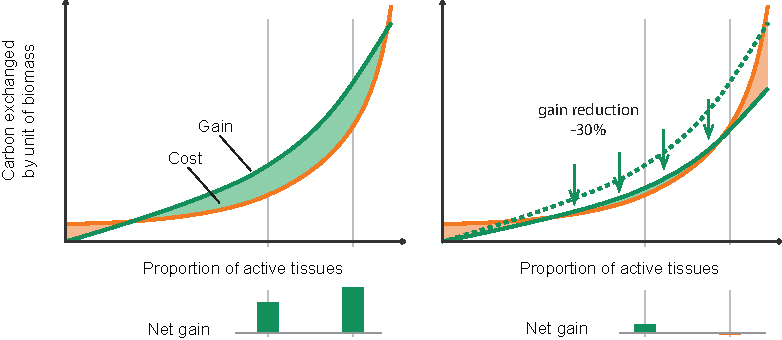
\includegraphics[width = \textwidth]{./2_PP/Figures/Variable/explain_assymetry.pdf}
\caption[Optimum strategy and resource availability]{\textcolor{myGreen}{Gain} and \textcolor{myOrange}{losses} curves along the allocation strategy axis for one organ. Left panel corresponds to a high resource availability, the right panel illustrates the effect of a 30\% loss of gain due to a reduction of the resource availability. The botton bar plots represent the net gain of two distinct phenotype in the two conditions.}\label{fig:asymmetric_gain}
\end{figure}

The maximum exchange rate influencing the slope of the gain function not only depends on the resource availability, but also the non limitation by the other organ or by regulation functions (see examples in \cite{lohier_analyse_2016}).

% why plasticity does not help.
When the limitation of the exchange rate is only dependent on the conditions, and the equilibrium is insured by the optimum RMF, in constant conditions the phenotypic plasticity cannot alter the optimum phenotype. This result supports the idea that plasticity should not induce a shift in the dominant strategy if the environmental conditions are stables.

% no consequences on the community identity.


%\paragraph{Static and dynamic gain}
%\paragraph{Who benefit from plasticity}
%
%Gains from the plasticity can be distinguished between static and dynamic gains. The lower value of the \textit{center of gravity} in conditions of low water availability under \textit{fixed-e"quilibrium} algorithm seems to indicate that conservative strategies benefit from plastic allocation more than exploitative species. However, this effect is mostly due to static gain as the optimum strategy does not change. This effect is due to a growth landscape flatter than in better conditions (more species within the 90-100 \% of maximum growth, lower growth difference with best strategy) and asymmetric, that has two effects:
%\begin{itemize}
%\item it reduces the growth gain for species with strategy close to the optimum, but not at the equilibrium (figure \ref{fig:optimum_shift} panel A);
%\item increases the potential gain (relative to less flat growth landscape) for species with strategies more conservative than the optimum (figure \ref{fig:optimum_shift} panel A).
%\end{itemize}

\paragraph{Static gain}

% static gain idea
The cumulative productivity of all species combined is largely improved by the plasticity for all parameter sets (see figure \ref{fig:total_BM}). However, the best total biomass is only improved for a fraction of these parameter sets (see figure \ref{fig:maximum_BM}), while it remains similar in most of others parameter sets between \textit{non plastic} and \textit{fixed-equilibrium} simulations. This observation supports the idea that the total biomass is mostly increased due to an improvement of plants with a non optimum phenotype, and not an improvement of the best phenotypes. Moreover, while the number of species reaching high performance levels increases with plasticity (corroborating the previous conclusion), the functional diversity does not increases. We can conclude that the phenotypic plasticity leads to a convergence of the plants toward good performance phenotypes. Therefore, the productivity gain provided by the plasticity comes mainly from the convergence toward the best fixed phenotype, and cumulative static gain.

This form of gain provided by the phenotypic plasticity can be called \textemph{static gain}, as it is caped by the best performing constant phenotype. It is illustrated in the figure \ref{fig:filter}. The gain only comes from the transition from a sub-optimum phenotype toward the best one (see  \textcolor{myOrange}{starting phenotype A}  shifting toward the green one). The gain can be quantify as the total biomass difference between the non plastic species (- - dashed line) and the plastic one (- continuous line).  In constant condition, the best phenotype cannot benefit from the plasticity because it has the highest growth rate along time and has no static gain (\textcolor{myGreen}{starting phenotype B}). 


\begin{figure}\label{fig:filter}
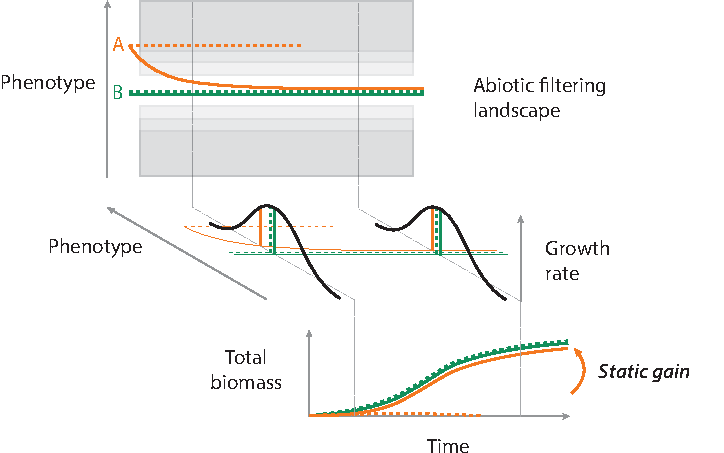
\includegraphics[width = \textwidth]{./2_PP/Figures/Rain/filtering.pdf}
\caption[Abiotic filtering in constant conditions]{Conceptual representation of the abiotic filtering in constant conditions and the illustration of the static gain. The top panel represent the abiotic filtering landscape with a central valley, and the trajectories of the species. The middle panel is the growth rate as a function of the phenotype for two positions in time. The bottom panel illustrates the growth curves for the different phenotypes. Two alternative position \textcolor{myOrange}{A} and \textcolor{myGreen}{B} represent a sub-optimum and the optimum position without plasticity (dashed lines). Alternative plastic trajectories are represented by continuous lines. }
\end{figure}

% abiotic filtering, constant filter
The static gain allows species to persist in environmental conditions that do not fit their initial phenotype (\textcolor{myOrange}{A -- continuous line}), and go through the \textemph{abiotic filter} while the non plastic equivalents \textcolor{myOrange}{A - - dashed line}) cannot. This reduction of the impact of the abiotic filter can have large impacts on the community properties.

% convergence idea This mechanisms does not consistently support functional diversity of the vegetative traits, but it can increase functional redundancy. The species diversity can be increased by this form of gain, and it may limit the the vulnerability of the community if multiple species have the function.

% other dimensions diveristy
%The functional convergence is obvious when only the vegetative dimensions are observed. But the functional diversity may be considered for other traits, therefore the promotion of species richness by the reduction of fitness differences can promote the functional diversity of the community. 


\paragraph{Niche widening}

The phenotypic plasticity of the RMF leads to an important widening of the potential niche. This is explained by the removal of one constraint of the niche. Indeed, with cost-free plasticity in RMF, the equilibrium is almost guaranteed for all species and the resource-use strategy is the only limitation of a species niche. Because the best proportion of active tissues is the same for a long portion of the gradient (high water availability)(see figure \ref{fig:gradient_strat_trend}), along the gradient most of best phenotypes share this resource-use strategy. Therefore, along this same gradient, if the RMF axis is ignored, the different species have equivalent phenotypes (except for a few first growing  days).

This niche widening has for consequence a higher niche overlapping. This overlapping can be translated into lower niche differences, as the niche are now discrimated only on one dimension, and into lower fitness differences as the species with similar strategies but different memories have close performances under plastic allocation. According to \cite{turcotte_phenotypic_2016} these two processes have opposed effects (see figure \ref{fig:plasticity-effect} in chapter \ref{part:literature}). On one hand the reduction of the niche differences diminishes the positive effect of the spatial heterogeneity on diversity. On the other hand, the reduction of fitness differences reduces the competitive exclusion of the non dominant species and limits the aboitic filtering. The current simulations do not allow to tell which effect will be the strongest at the community scale. The cost of plasticity should nevertheless ensure some degree of niche differentiation. In addition to these two effects, the widening of the potential niche corresponds to a reduction of the abiotic filtering pressure, and should promote the diversity as more species can potentially invade an habitat. 

\paragraph{Competition effect}

The reduction of the abiotic filtering implies a potential increase in the biotic filtering due to the limited carrying capacity of the habitat. This could raise the competition intensity, especially at the beginning of the growing season, and eventually change the dominant species if this increase is strong enough to alter the competition outcome toward more competitive species. Unless the eventual new dominant species has a dramatic effect of the overall productivity or diversity, the effect of the phenotypic plasticity through the competition should be positive or null on these properties. But because the phenotypic plasticity does not alter directly the optimum phenotype in temporally fixed conditions, the impact on the dominant resource-use strategy should be rather limited.

\paragraph{Meta-community dynamics}

While the effects at the community level are still hard to defined, the phenotypic plasticity can alter the dynamic at the meta-community scale. Phenotypic plasticity, by reducing the abiotic filtering effect, allows for stronger link between the communities as the chance to transfer from one community to another are higher. Therefore this mechanism has a positive effect on the stability of the ecosystem as species from unperturbed communities can invade, and partly sustain the properties and services of the perturbed community.

In a context of global change, to survive two options are possible: (1) migrate to new habitat with suited conditions, (2) adapt to new condition in the same habitat. In this context, the phenotypic plasticity facilitates both the adaptation to new conditions in the same spatial habitat and the adaptation to a new habitat that match the ideal conditions only to a certain degree. By facilitating the adaptation to new conditions or habitat, the phenotypic plasticity reduces the relative importance of climatic variables compared to the competition as already suggested by empirical results \parencite{alexander_novel_2015}.

%
%This widening is, however, asymmetric because there is a transition of the limitations that define a species niche. Without plasticity, in a given homogeneous environment, the optimum phenotype is defined by both the adequate resource-use strategy and the balance between organs. With costless  Conservative species are less efficient in high resource availability conditions, while exploitative species are more efficient. 
 
% If cost are low, the effect is likely to reduce potential species diversity. An established species can, thanks to static gain, maintain relatively high growth rate in an habitat where the balance is different but the optimum strategies closed. This is particularly true for rich environment where the optimum strategy for roots is quite stable. The effect on coexistence is better illustrated with an example. Given two species, \textit{species a} and \textit{species b}, with optimum strategy (PAR) and RMF for two distinct conditions, respectivelly \textit{A} and \textit{B}, in a heterogeneous environment composed of majoritarely condition \textit{A} and minorly condition \textit{B}, ... where do I go with that ? ... 
 


%Reduce the structural role of spatial heterogeneity. Favour seed dispersal strategies. In high resource conditions, the resource levels do not matter much (non linearity of the optimum along gradient) but balance does, plasticity could reduce species richness, unless cost of plasticity. Unless not enough space to really be a niche (rare conditions): give opportunity to some species to extend their niche.

%\paragraph{Fitness evenness}
%
%The phenotypic plasticity reduces the importance of the filtering effect of abiotic conditions by increasing the flexibility of one of the niche axis (the balance between shoot and root activities). This increase in growth evenness between species will certainly impact the community properties. Multiple effects can be anticipated on the mechanisms that affect these properties. The first effect
%
% 
% However, what is the effect on coexistence mechanisms. The widdening of the potential niche of numerous species, Probably negative: so hard to tell effect on coexistence.


\begin{figure}\label{fig:rain_pl_effect}
    \classiccaptionstyle
\sidebysidecaption{0.60\textwidth}{0.3\textwidth}{%
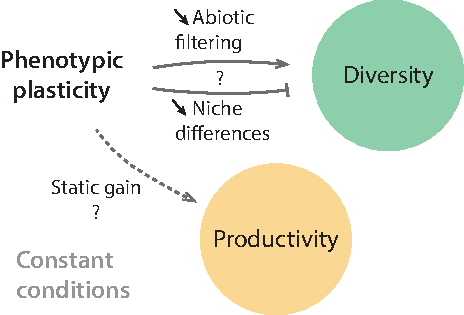
\includegraphics[width = \textwidth]{./2_PP/Figures/Rain/rain_pl_effects.pdf}
}{
\caption[Effect of plasticity in constant conditions]{Effect of the phenotypic plasticity on the main properties of the grassland communities in constant conditions.}
}
\end{figure}

\textbf{In constant environmental conditions, the phenotypic plasticity already has an impact on species performances and interactions through the static gain it provides to species with the good resource-use strategy, but a wrong estimation (memory) of the resource availability. It increases the fitness evenness of species by reducing the abiotic filtering dimensionality down to the resource-use strategy, axis not influenced by the plasticity. This leads to a convergence of the phenotypes and a widening of the potential niche. The effects at the community level are hard to anticipate, but they will be largely dependent on the competitive interactions and how they are affected by the plasticity. The reduction of the abiotic filtering will likely increase the species diversity, but the functional diversity might not follow this trend due to functional convergence. The effects on the other component of the ecosystem properties cannot be fully determined and greatly depend on the outcome of the competitive interactions. In temporally heterogeneous conditions, the phenotypic plasticity may play a larger role and greatly mediate the community's properties.}


%\textbf{Mostly static gain, but even if there is gain, increases the potential niche of species that are settled. Bigger niche: favourable for conservative species of rare habitats.\\
%Hard to tell anything on coexistence, except wider niches}



\subsection{Results: gradient of heterogeneous precipitation conditions}

This part of the chapter present the results at the individual scale along a gradient of temporal increasing variability of the underground resource (increasing negative slope of water influx).

\paragraph{Productivity}
The maximum biomass (relative to the \textit{non plastic} best performance in constant watering conditions) decreases along the gradient for all allocation algorithms (see figure \ref{fig:variable_BM}). The \textit{non plastic} algorithm show a drastic drop after the fourth level of variation, while the fixed-trait algorithms show better performances in this part of the gradient. The \textit{plastic-optimisation} algorithm show low growth for all conditions, but a more stable performance.

In contrast with the stable conditions (see previous results) the plasticity provide, in non constant conditions an great improve in the maximum biomass for most parameter sets. 

\begin{figure}\label{fig:variable_BM}
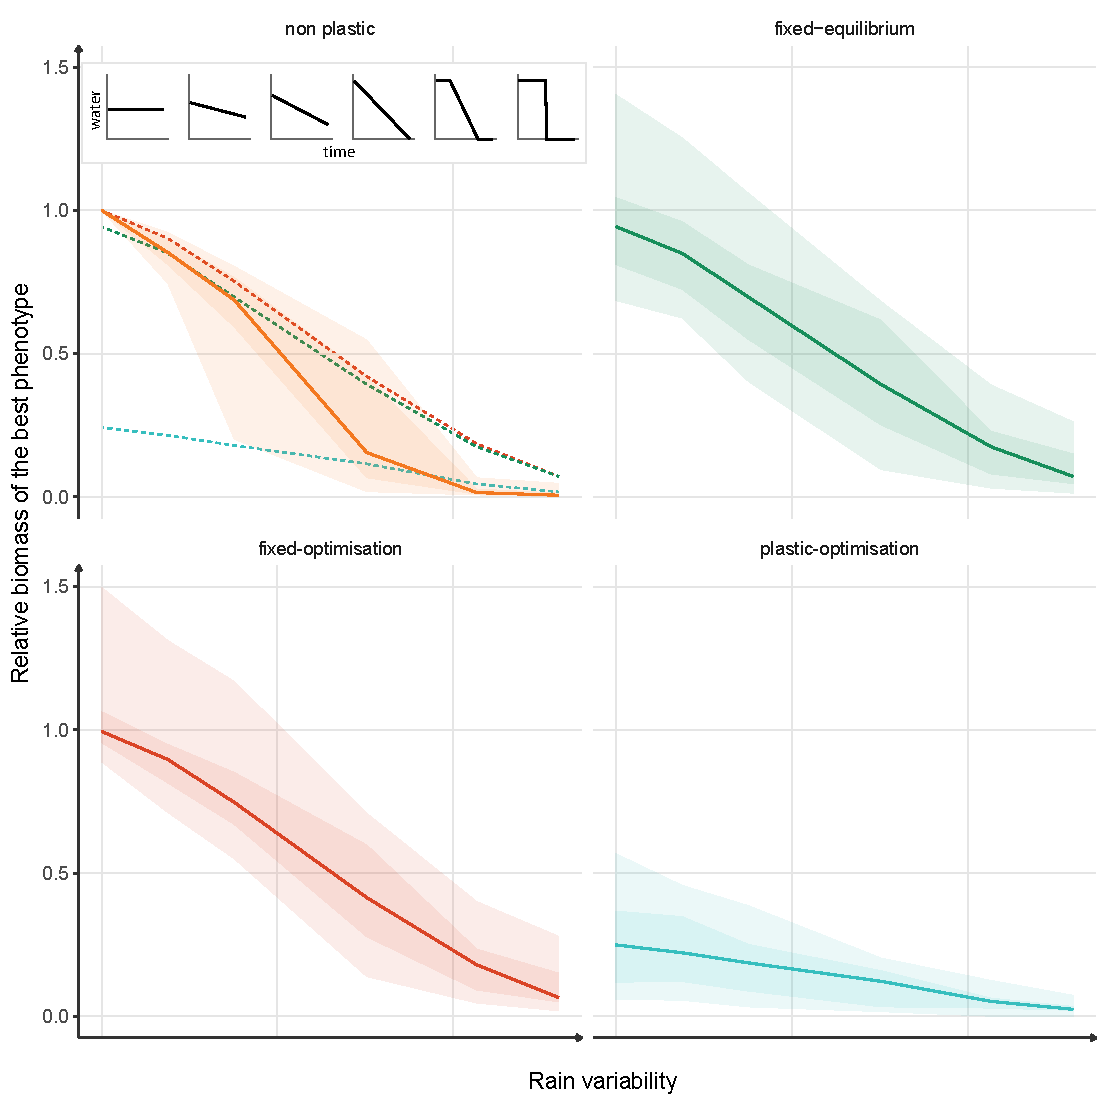
\includegraphics[width = \textwidth]{./2_PP/Figures/Variable/var_relnone_BM_trend.pdf}
\caption[Biomass variations along a gradient of resource variability]{Biomass variation of the best performing species along a gradient of resource variability for four plasticity treatment. The upper panel of the top-left frame illustrate the water influx as a function of time along the variability gradient. The dotted lines in the top-left frame indicate the median biomass for the other three algorithms. }
\end{figure}

%
%Along the temporal heterogeneity gradient the median biomass of the optimum phenotypes decreases under all allocation algorithms when the variability increases despite the same mean water influx. The amplitude of reduction varies with the allocation mechanism: \textit{non plastic} algorithm shows the largest decrease while \textit{fixed traits} algorithms show slower decrease. \textit{Plastic- optimisation} simulations have more constant performances with low initial performances in constant condition (between 5\% and 55\% on the \textit{non plastic} simulation), but they end with slightly better performances than \textit{non plastic} simulation for the extreme case of variation (two extreme regimes).

\paragraph{Identity}

In addition to a reduction of biomass, the increasing slope of the water influx reduction lead to a shift of the optimum strategy in \textit{non plastic} simulations (see figures \ref{fig:variable_strategy} \&  \ref{fig:variable_trajectories}) toward more conservative strategies. The median optimum value shifts from 0.85 to 0.75 then 0.35 in extrem conditions. This reduction of optimum toward more conservative strategies is offset in most of \textit{fixed-equilibrium} and \textit{fixed-optimisation} simulations where the median optimum value for the PAR stays above 80\%. Only a small reduction (around 25\%) of the 5th and 25th percentiles of the optimum root strategy can be observed between the extreme conditions for these two algorithms.

\begin{figure}\label{fig:variable_strategy}
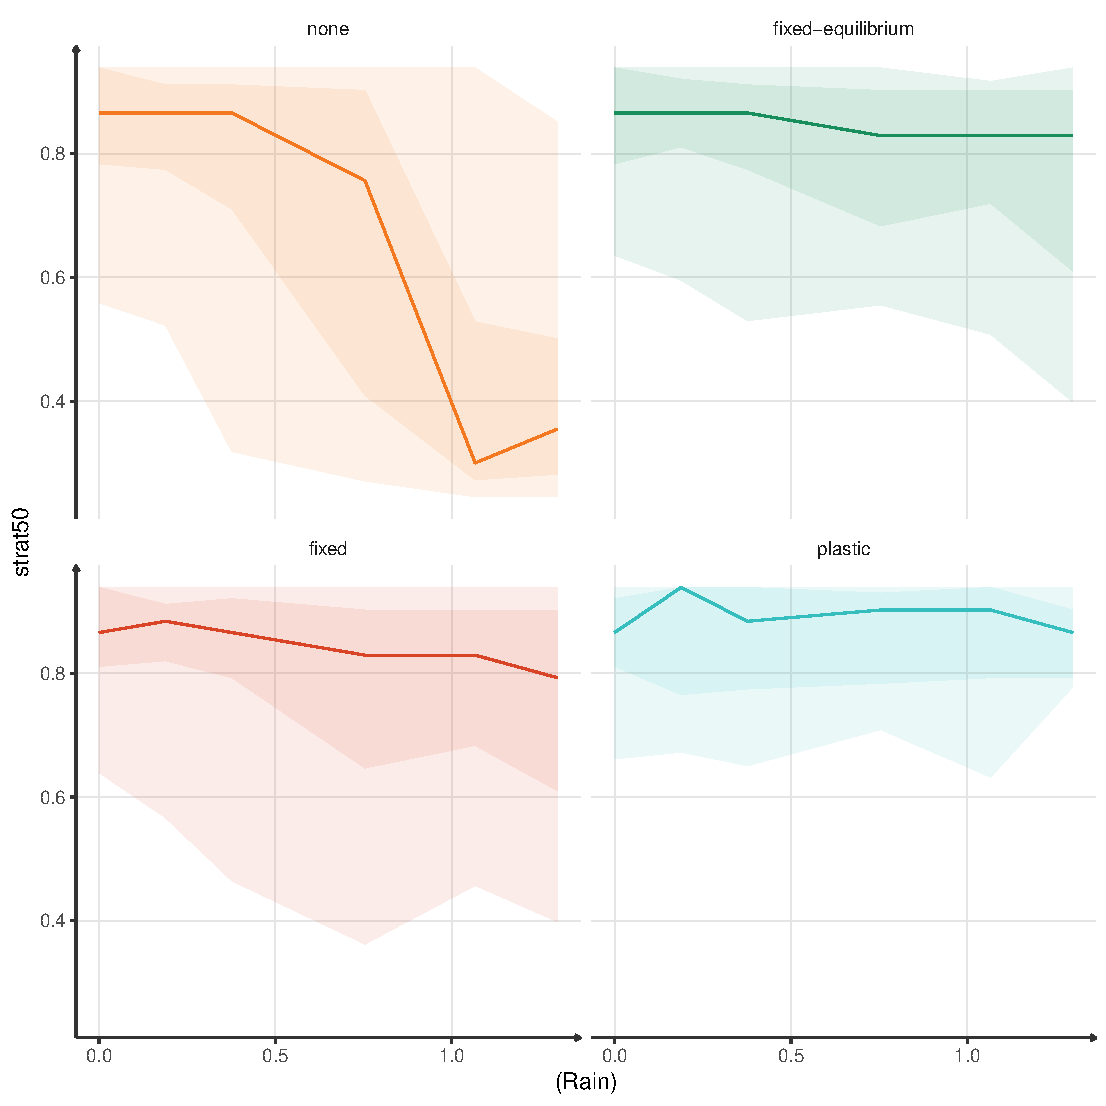
\includegraphics[width = \textwidth]{./2_PP/Figures/Variable/var_strat_trend.pdf}
\caption[Strategy shift along a gradient of resource variability]{Strategy (PAR: proportion of active tissues in root) shift of the best performing species along a gradient of resource variability for four plasticity treatment. The dotted lines in the top-left frame indicate the median PAR for the other three algorithms.}
\end{figure}

 This shift in optimum strategy can better be observed on the plan of the proportion of active tissues in root (PAR) and root mass fraction (RMF) in figure \ref{fig:variable_trajectories} where all trajectories\sidenote{trajectory of the optimum, not of the species.} along the variability gradient are plotted. \textit{Non plastic} allocation trajectories by a linear shift toward more conservative strategies with higher allocation to roots, while \textit{fixed-equilibrium} and \textit{fixed-optimisation} trajectories are non linear and can be divided into two phases: (1) increase in RMF, (2) reduction of PAR. \textit{Plastic-optimisation} algorithm shows no consistent pattern in trajectories.


\begin{figure}\label{fig:variable_trajectories}
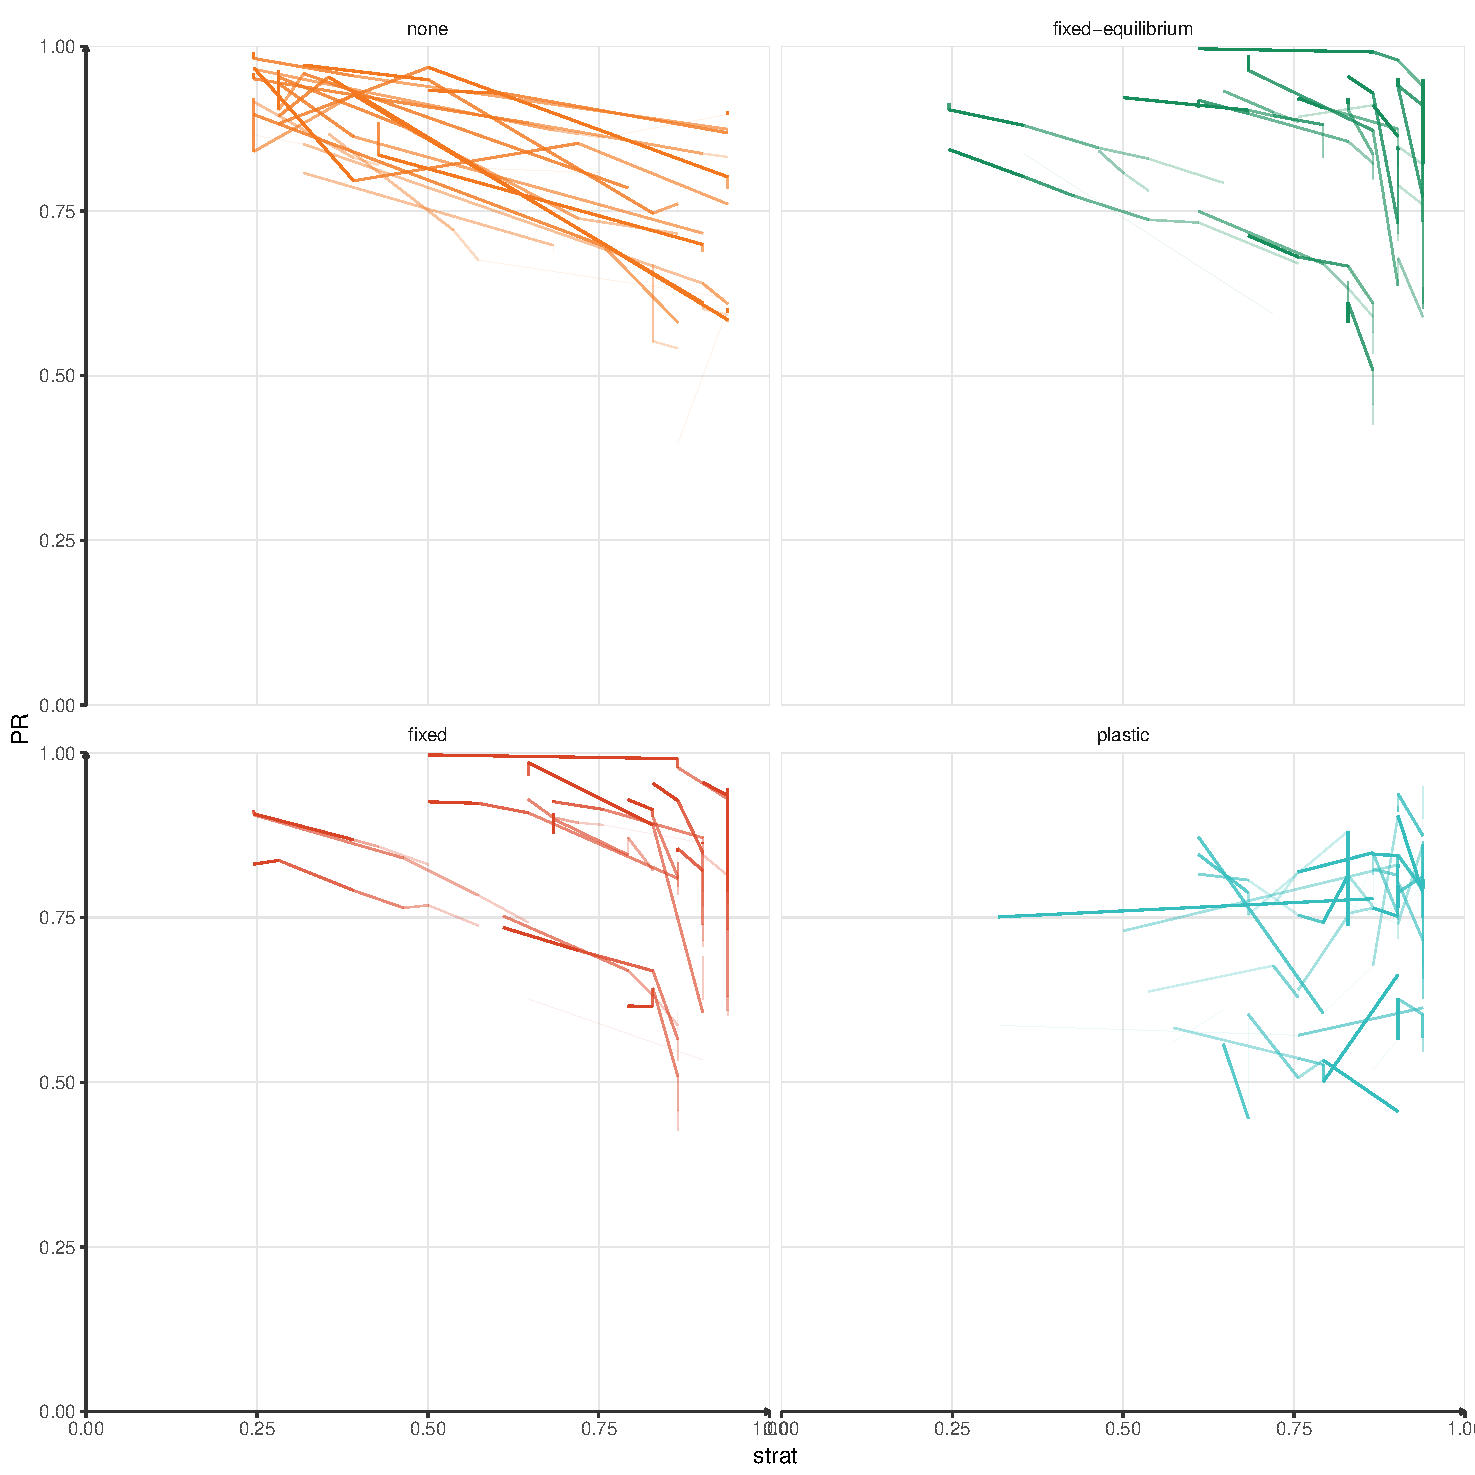
\includegraphics[width = \textwidth]{./2_PP/Figures/Variable/var_2D_strat_dyn.pdf}
\caption[Best phenotypes along water resource variability gradient]{Best phenotypes along water resource variability gradient. Thinner lighter lines indicate low water variability, while the thicker lines indicate strong temporal heterogeneity.}
\end{figure}

\paragraph{Diversity}

%As previously seen, plasticity can affect diversity in a drastic way, reducing the functional diversity by contracting the phenotypic space, but also increasing the potential species diversity by the same mechanism. The effect of static gain\sidenote{refers to the gain due to convergence toward a good static phenotype and no temporal changes.} and dynamic gain must be disentangle. The 


Along the gradient, the performance and the identity of the bet phenotype were greatly altered by the water variability, but the phenotypic plasticity mitigate these effects. The number of species is fairly stable for all alogrithms but the \textit{non plastic} that show an improvement in species diversity. The fixed allocation algorithm have between 15\% \& 20\% of the species within the 90\%-100\% range of the maximum biomass for the conditions, while the \textit{non plastic} allocation show this level only of the extreme variable case, but otherwise is limited to a few percents. The functional diversity is stable along the gradient and is similar for all agorithm (\textit{plastic-optimisation} algorithm being exclude)(data not shown).

\begin{figure}\label{fig:variable}
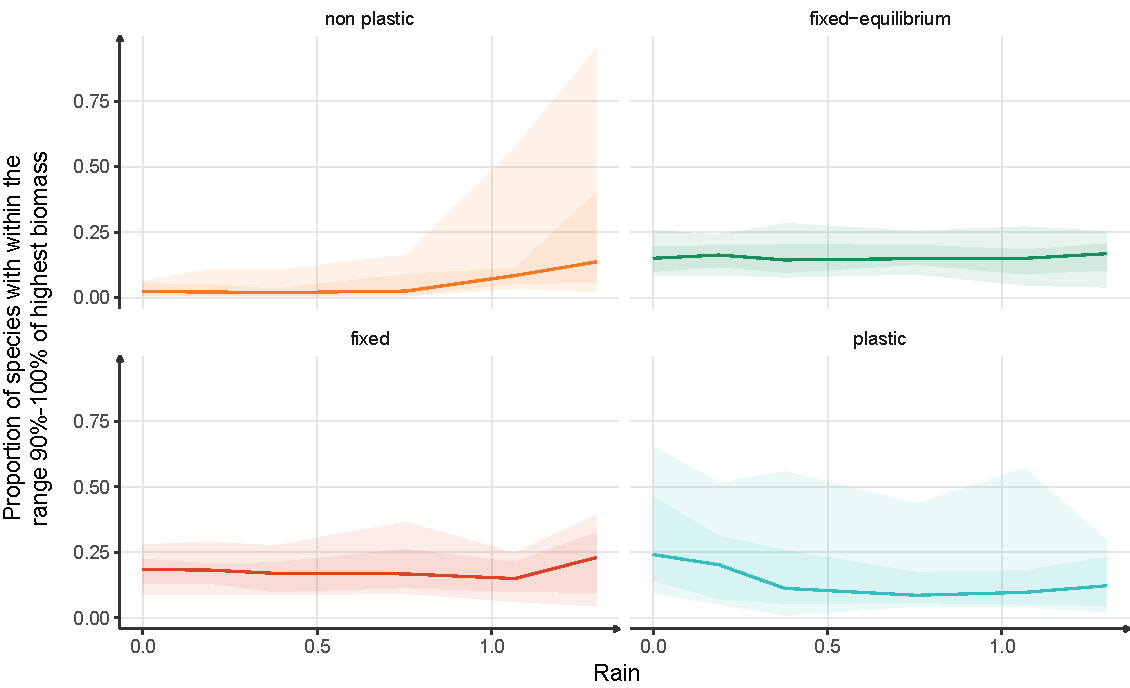
\includegraphics[width = \textwidth]{./2_PP/Figures/Variable/var_spdiv_trend.pdf}
\caption[Species richness of the best performing species along a water resource variability gradient]{Species richness of the species within the range 90\%-100\% of highest biomass for any given condition (parameter and precipitation) along a water resource variability gradient.  Colour distinguishes plasticity treatments: \textcolor{myOrange}{- \textit{non plastic}} \&  \textcolor{myGreen}{- \textit{fixed-equilibrium}}.}
\end{figure}

%Changes in optimum, but does it affect eveness ? Same pattern as before with tehe trade-off between species and functional diversity. What happen if you filter down stuff ?





\subsection{Discussion: gradient of temporal variations}

\paragraph{Resistance to variability}

Before analysing the effect of the different plastic algorithm, the \textit{non plastic} simulations show interesting patterns. The first thing inform us on the relative importance of growing versus surviving. Because the mean water influx over the simulated period is conserved, an increase in the influx negative slope means that during the first half the plants have more available water, while they have less during the second half (relative to constant influx. The decreasing biomass along the gradient suggests that this additional water (and therefore potential growth) does not compensate for a reduction in growth during the drought period. Therefore, it is more important for the plant fitness to limit losses during scarce period instead of maximizing growth during favourable periods. 

\begin{marginfigure}
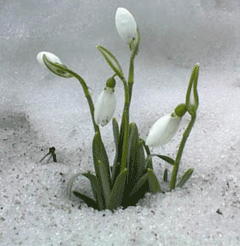
\includegraphics[scale=1]{./2_PP/Figures/Variable/GalanthusNivalis.png}
\caption[\textit{Galanthus nivalis}]{\textit{Galanthus nivalis} is an example of species that develop early in the season to avoid competition and benefit from the high resource availability.}
\end{marginfigure}

However, this conclusion should be mitigated by the fact that some reproduction strategy still can benefit from early exploitative strategies and there are not considered here because the success is measure by the biomass afeter 100 days. This effect can be explained by the fact that even the most exploitative species are not fully developed when the resources are the most available, therefore the potential compensation by an early growth is limited. This is the case in the context of mountain grasslands, and some specific life cycle strategies take advantage of this particularity like the \textit{galanthus} species (see figure \ref{fig:galanthus}) with early development\parencite{schroder_modelling_2014}, or development from bulb that allows for an early and rapid growth.

% selection of more conservative species, plus reduction of prod that show non compensation mech. -> best strategy during the bad period, but no
%The selection of more conservative strategy at the end of the gradient confirms the importance of maintaining growth (or reducing losses) during the period of lower water availability, and demonstrates the higher resistance of the conservative strategy to the resource fluctuations.

The reduction of biomass along the gradient, even in plastic conditions, supports the idea of a lack of compensation mechanisms between favourable and unfavourable drought periods. In addition to this conclusion, the better performances of the conservative species in low water conditions relative to exploitive species (see figure \ref{fig:gradient_strat_trend}), suggests that the best strategy is determined by the optimum resource-use strategy of the most important growth period (the drought period). However, another mechanism can be involved and is relative to the capacity of the species to perform well both in conditions that suit its phenotypes, and in conditions that do not suit its phenotype. In a variable environment, the phenotype does not match conditions different from its niche center because of the optimum resource-use strategy may change, or because the balance between root and shoot activity changes. Both can be important. As said, the former is suggested by previous results, however under plastic allocation the optimum resource-use strategy is maintained at high values of proportion of active tissues. Therefore, the difference in optimum resource-use strategy along the gradient cannot explain alone why conservative strategy are better in contrasted environment. The other explaining mechanism is a better resistance to variability from conservative species, relative to exploitative. The variability in water conditions while the light conditions are fairly constant leads to a shift in the balance in the availability of the two resources. If the phenotype is fixed, a shift from balanced conditions (equilibrium between shoot and root is respected for the given phenotype in these conditions) to unbalanced conditions (no more equilibrium for the same given phenotype) can be seen from the plant perspective leading to a reduction of the overall gain function stronger than the actual decrease in resource, because the non limiting organ is in over-capacity. Because they have a higher resource-use efficiency (see figure \ref{fig:asymmetry}), conservative species can cope with this reduction in gain due to unbalanced organ activities. Therefore, in variable conditions, the optimum strategy shifts toward conservative strategies that have the capacity to support greater exchange rate reductions. Under plastic allocation, the equilibrium is maintained, reducing the need for a strategy resistant to resource fluctuations. This illustrated by the figure \ref{fig:variable_trajectories} that shows along the variability gradient a direct shift toward more conservative root strategies and greater root allocation, while under plastic allocation, the shift toward conservative strategies is delay for stronger availability gradient, but the RMF shows larger values (they are measured at the end of the simulation, when the water availability is reduced).

\textbf{The plasticity of the RMF axis allows plants to cope with resource availability and maintain exploitative strategies. These strategies are more sensitive to changes in resource levels under \textit{non plastic} allocation than the conservative species that benefit from a rgeater resource-use efficiency.}


%Therefore, to the given plant, the decrease in resource is stronger than the actual decrease in resource, and the optimum resource-use strategy shifts toward a more conservative strategy than a balanced phenotype would require. 

% message: it is not because the optimum change, it is because the conservative species are more resistant to variability.

%
%\begin{figure}
%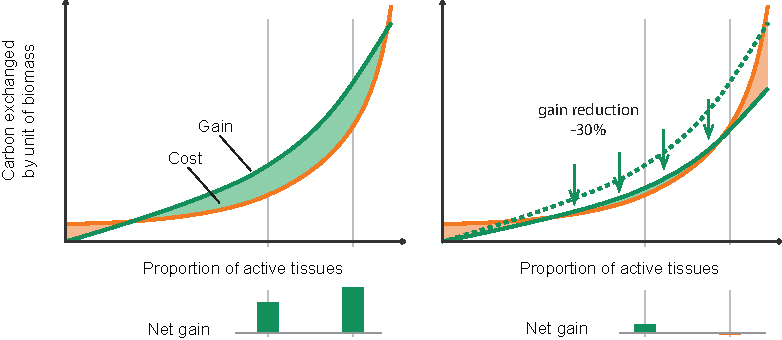
\includegraphics[width = \textwidth]{./2_PP/Figures/Variable/explain_assymetry.pdf}
%\caption[Assymetric gain from gains and costs perspective]{Gain and lost curves along the allocation strategy axis for one organ. Left panel corresponds to the gain and cost in a situation where the equilibrium is maintained, the right panel illustrates the effect of a 30\% loss of gain due to unbalanced exchanges between organs. The botton bar plots represent the net gain of two distinct phenotype in the two conditions.}\label{fig:assymetric_gain}
%\end{figure}

\paragraph{Who benefit from the plasticity?}
% who wins -> assymetric and impact of the identity
While the phenotypic plasticity does not provide any clear advantage to a type of species in constant conditions, in changing conditions the phenotypic plasticity benefit to the exploitative species that are able to maintain good performances in contrasted conditions (see figure \ref{fig:variable_strategy}). Because the plasticity gain is assymetric, the phenotypic plasticity alters the identity of the community and promotes exploitative species in variable conditions while conservative species are favoured under \textit{non plastic} allocation. In a more theoretical view, the plasticity can be seen as an alteration of the strength of the stress as shapping factor of community \parencite{grime_evidence_1977}. If the plasticity allows the exploitative species to better support stress, in modelling studies that do not take into account such plasticity, the amplitude of the stress needed to see a shift in the community identity may under-estimated.

% effect on the stability of the community
This asymmetric gain should favour already established species as it lowers the perturbation effect of climatic fluctuations. This stability is interesting for the maintenance of the ecosystem properties and services provided by the mountain communities. It also support the idea of a greater resistance to climatic event that are expected to be more frequent under the climate change. 

% Why is that ? absolute and relative, the role of the euilibrium

\paragraph{Dynamic gain and stability}



\begin{figure}\label{fig:variable_filter}
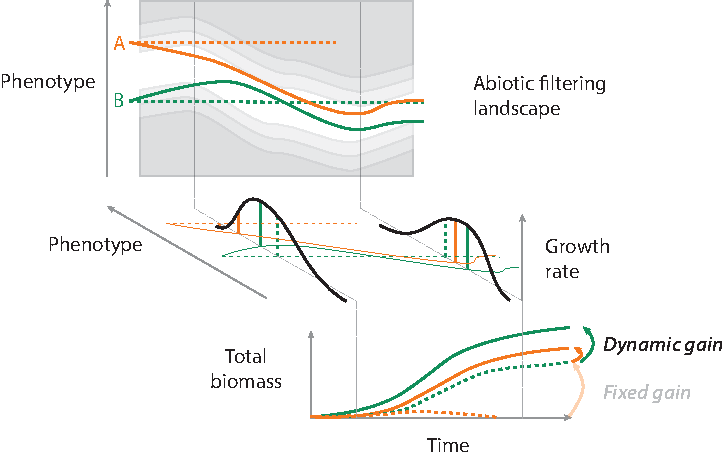
\includegraphics[width = \textwidth]{./2_PP/Figures/Variable/variable_filter.pdf}
\caption[Abiotic filtering in temporally variable conditions]{Conceptual representation of the abiotic filtering in variable conditions and the illustration of the dynamic gain. The top panel represent the abiotic filtering landscape with a sinuous valley, and the trajectories of the species. The middle panel is the growth rate as a function of the phenotype for two positions in time. The bottom panel illustrates the growth curves for the different phenotypes. Two alternative position \textcolor{myOrange}{A} and \textcolor{myGreen}{B} represent a sub-optimum and the optimum position without plasticity (dashed lines). Alternative plastic trajectories are represented by continuous lines. }
\end{figure}

%Because the shift in non plastic condition is due to vulnerability, and not optimum strat during the most growing period. (there could be some compensation, leading to best exploit phen,, even if conservative are indeed more perf in drought period).

% What what consequences for the productivity (cite maire)




\paragraph{About diversity}

%
%\paragraph{Improvement in variable conditions}
%Plasticity has a positive effect on exploitative strategies in low resource availability conditions. As said earlier in the document, plant performance depends on multiple things: the effectiveness of organs, the global resource availability and the equilibrium. 
%% Here talk about the spatail heterogeneity:
%If plasticity improve the performance of the exploitative species, it is unlikely to be because of the contraction of the space since it is the optimum only that is looked at. Also means it is probably dynamic gain, it the filter was static, plasticity shouldn't have change much. And there is gain, even in the high end of the gradient where the optimum does not move, saying that the optimum is fairly conserved despite increase in resource (but low resolution of the strategy space, and match the function). 
%
%% From theere, talk about the variable rain input.
%Change in optimum strategy can be explained by: an assymmetry in efficiency (better a but more conservative in exploitative favourable conditions than exploitative in conservative favourable conditions) or an assymetry in inbalance cost (better be inbalanced when conservative than when exploitative). The first option is not consistent with previous results (see subsection \ref{section:landscape}, figures ...) that show higher fitness for species more exploitative than the optimum, compared to species more conservative. In the other hand, following results show positive effect of functional equilibrium over conservative strategies. Nevertheless, this effect certainly results from an artefact and the contraction of the phenotypic space not in favour of exploitative strategies. The sensitivity of exploitative strategies to low conditions is visible in figure \ref{fig:gradient_optimum_strat}
%
%Shift of RMF then strategy explain quite well that the equilibrium is more important than the resource usage and the organ efficiency. How does that inform us on the real world ?
%
% - potentially reduces the meta community diversity if spatial heterogeneity has a less drastic effect on strategic dominance. - talk about that in diversity part
%
%/!\\ may come from a lack of coordination with shoot. Since shoot activity is suppose to be relatively high. == might not have besn a good choice to look only at root strategy. But, since there is adjustment of RMF that allow to maintain equilibrium and resource usage, it should be fine to interpret these results.
%
%\textbf{Phenotypic plasticity give exploitative species an advantage in variable conditions because their growth rate rely more on productivity and therefore equilibrium than conservative species. }

% Indirect effect of identity on diversity, mention it but more a perspective.

%\paragraph{Heterogeneity of response}
%
%Kichenin (different response to gradient) Doesn't work in this framework: Not so sure about that: depending on your initial memory plants show directional changes toward one phenotype. Yeah, but they should have converged for other conditions too... So, it doesn't work. Might be explained by:
%\begin{itemize}
%\item different conditions: because heterogeneity and habitat selection, or changes in competition hierarchy;
%\item different ways to tackle changes on one dimensions;
%\item different weights between mechanisms impacting composite traits, because of the different traits.
%\end{itemize}


\begin{figure}\label{fig:variable_pl_effect}
    \classiccaptionstyle
\sidebysidecaption{0.60\textwidth}{0.3\textwidth}{%
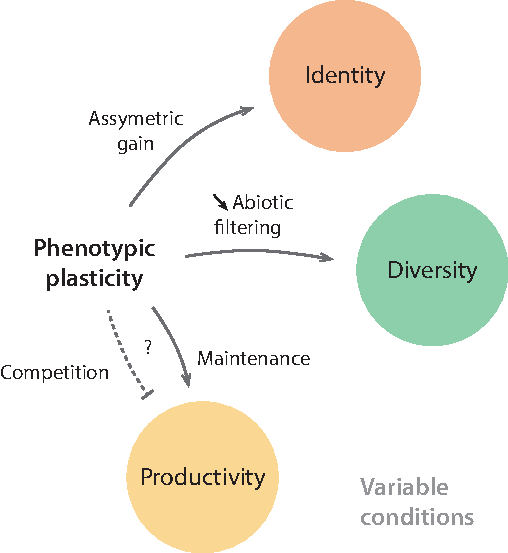
\includegraphics[width = \textwidth]{./2_PP/Figures/Variable/variable_pl_effects.pdf}
}{
\caption[Effect of plasticity in variable conditions]{Effect of the phenotypic plasticity on the main properties of the grassland communities in variable conditions.}
}
\end{figure}


\textbf{The phenotypic plasticity implemented in \model improve the relative performance of multiple strategies by concentrating the plant toward a subspace of higher performance for most of plants. Convergence to a smaller subspace can be assimilated to reduction in phenotypic diversity, but it reduce performance heterogeneity and should favour local plant diversity. However, this effect should be limited by plasticity cost. Indeed, if the growth gain due to plasticity is only static, any species with a fixed phenotype closer to the optimum than the focus species has a better growth rate and exclude the focus species.
. a few words on dynamics... Meta-community diversity is however reduces by the reduction of potential axis for niche differentiation. Plasticity costs and limits should play major role in the balance between these mechanisms. Community level simulations are needed to further understand the cumulative role of competition, spatial and temporal variability and plasticity costs on phenotypic plasticity influence on plant community dynamics.}


\section{Other plasticity patterns, alternative implementation and stability of results}

% ! ! ! 
% Talk about how the model informs on the effect of plasticity:
% do not really mimic the reality since the plasticity can be turn on and off, but when there is an effect, it tells us how to modulates the other effects (stronger if opposite, or less strong if in the same direction), and help us identify the real sources and amplitude of effect.
% Nevertheless, could it not tell us how real plasticity impact communities when there are evidences of plastic vs non plastic plants... ?

\subsection{Resource foraging and architecture plasticity}

\paragraph{Resource foraging}

% shoot, forest

% etiolement

% roots


\paragraph{Architecture plasticity}

% how 

% benefits

% drawbacks



\subsection{Temperature gradient, phenology and ontogeny}

\paragraph{Temperature and altered phenology}

% increased biomass

% change leaves, but mainly phenoloty and reproduction

% often goes with other variables: integrative response.

\paragraph{A matter of reference}

% plasticity is relative

% facility to measure, external rather than internal

\paragraph{Ontogeny}

% respond to BM, need to understand why to model?


\subsection{Alternative implementation and robust observations}

\paragraph{Stress-based plasticity}

% what? and how? stress, response, reset, memory, recovery

% benefits stable phens, take into account vulnerability, not only optimum
% multiple stresses, different sterss level (already posible, even if only 1 tau value in this implementation of MG

% drawbacks: hard to integrate in a global gain function, and to determine value of composite traits, multiply species specific parameters -> calibration is harder (but can start with common parameters)

\paragraph{Reaction norms}

% what and how ?

% benefits

% drawbacks

\paragraph{Heterogeneity of responses}

% consistent 


\paragraph{Robust observations?}
% static and dynamic gain

% asymmetry for exploitative

% niche overlapp: -> increases potential diversity and competition,
% reduces functional diversity ?


%
%
%\subsection{Plasticity: new functional diversity}
%
%functional diversity of plastic traits? Should them be excluded?
%
%Impact of traits, and abundances: the need to account for it!
%
%May still be useful especially for invasion, and works well despite low flexibility (see \parencite{forsman_rethinking_2014}. May allow more diversity if some correlations with other non plastic traits.	
%
%\subsection{Plasticity as a strategy: cost and correlations}
%
%\paragraph{Who benefit from plasticity?}
%
%\paragraph{Cost of plasticity}
%
%and limits ? what about exhaustion
%
%\paragraph{Plasticity as a strategy}
%One of the argument to say this is new, however not really explored, neither with plasticity cost perspectives (a bit with plasticity limits) or with tau. However, used extreme cases: give better understanding and necessary before finer analysis. Still, there are hypothesis on the effect on diversity and the role in phenotypic stability (attention: isn't it just because the formulation of projection is wrong that we can make these conclusions ?).
%
%
%
%\subsection{Plasticity and competition: changes in interactions}
%
%\paragraph{Extended interpretations}
%What about the continuous $\tau$ gradient ?\\
%
%What about interactions and cycles ? Little has been discussed on the dynamic of the resource and how it could affect coexistence. Imagine that with cycle, reproduction timing has an importance here...
%
%
%plasticity will change: performance, sensitivity and impact of the resource.

%\section{From individual response to community dynamics}

% Use these notes to extend the discussion and add some outlooks
%
%\section{Niche response}
%
%
%Obj1: understand how resource use mechanisms and allocation algorithms shape the environmental potential niche in the context of the model.\\
%H1: strategy and memory affect niche in two ways if we suppose they are independent: shape and position. Strategy mostly affect shape (width and height) while memory (and so root:shoot ratio) affect mostly position.\\
%H1': there is strong link between strategy and memory in the case of optimisation allocation that increase niche height and might reduce its width.\\
%Obj2: understand the role of plasticity on the niche and if the effect in the same for all strategies/memories.\\
%H2: the plasticity increase niche width but not height (as phenotype is optimum at the center of the niche where memory match the resource availability).
%
%Stability and efficiency trade-off. Niche heigh and width and relationship with the strategy. How does plasticity affect that ? Does it increase the height and widen niches ? What does that mean for coexistence ?\\
%Hopefully higher niche would go with unstable niche.
%%
%%\section{Transitivity and competition}
%%1 vs 1 interactions\\
%%Is the resource competition transitive ? How does niche widening impact that, does plasticty change competition interaction. Is it related to the trait distance ? (don't think so)
